% binding info: NO NOTEBOOKS OR RING BINDERS, proefssional appearance, non-paper cover, bound. 8.5x11 w/ 1 inch margins, left side 1.5in margin.

% This is a test comment. So stop reading it you piece of shit

% text formatting info: The paragraphs are to be fully justified (both left and right sides). New paragraphs may begin by indenting the line or by not indenting but leaving a space. However, DO NOT do both. The body font must be Times Roman, Arial, Helvetica, or be approved by the instructor with a font size of 10-12 pts. Heading fonts can be no larger than 20 pts. The document must be single-spaced and printing can be single or double sided. Color printing is optional and left to the discretion of the groups.

% sources info: 5. The appendix must contain written authorization (emails, letters, or explicit permission citations) for rights to include or use copyrighted content. 6. All copyrighted contents must display the content’s origin or author, and an appropriate phrase such as “reprinted with permission.” 

% citing info: 7. All elements of the document that support the written text, such as figures, table, illustrations, code segment, charts, etc., must be cited in the body of the text, and the citation must appear before the element is shown. Supportive elements cannot begin a chapter, section, or paragraph. All supportive material must be captioned, which include the element name and number and a description. If you do not author the element, the caption must contain wording identifying that you have permission to use the element. The actually permission authorization must be included in the appendices.

% reference format info: 8. Your document should contain a “References” section at the end that lists all of the source material cited in your document. The references should be listed in the order that they first appear in your document in a format like the following (first is a book, second is an article): [1] J. Hennessy and D. Patterson. Computer Architecture: A Quantitative Approach, 5 th edition, Morgan Kaufman publishers, 2014. [2] M. Heinrich et al. “The Performance Impact of Flexibility in the Stanford FLASH Mujltiprocessor”, In Proceedings of the 6th International Conference on Architectural Support for Programming Languages and Operating Systems (ASPLOS), pages 274-285, 1994

% citation formatting: When citing the references in the text use a non-breakable space (e.g. Ctrl-shift-space in Word, \&; in HTML) before the citation and then square brackets and the number: Some researchers say that the occupancy of the node controller is the parameter most critical to the performance of the overall machine [2]. If you want to cite multiple references at once just separate them by commas like so [1,3,7].

\documentclass[a4paper,10pt]{article}
\usepackage[utf8x]{inputenc} 
\usepackage{graphicx}
\usepackage{float}
\usepackage{listings}
\usepackage{geometry}
\usepackage{helvet}
\usepackage{soul}
\usepackage{url}
\renewcommand{\familydefault}{\sfdefault}
	\geometry{
	%letterpaper,
	%total={8.5in,11in},
	%left=1.5in,
	%top=1in,
	%right=1in,
	%bottom=1in
}

%opening
\pagenumbering{roman}
%1. Cover page with title, group number, team members, date, and any other relevant information, such as participating organizations and sponsors.
\title{Group 12 Project Final Design Document}
\author{Eric Momper, Peter Lomason, John Barber}
\setlength{\parindent}{0pt}
\begin{document}
	
\maketitle
	
	\pagebreak
	\tableofcontents
	\pagebreak
\pagenumbering{arabic}	
\section{Executive Summary}
The relationship between psychology, therapy, and virtual reality is no new concept. Benefits which can be derived through the use of virtual reality as a treatment option are vast 
and already well researched with many successful studies and experiments supporting this type of therapy. A caveat to this success is that most of the treatment is carried out as research, 
at limited locations, or on a very exclusive basis.
\par~\\ 
This is due to a number of factors including the available openings for research, cost of the hardware and software involved, and locations of the few companies which professionally offer virtual reality therapy. Psychological and social factors also play a role in the underwhelming prevalence of virtual reality for psychology.  PsychVR aims to remedy this problem by offering a suite of treatment environments targeted at some of the most prominent psychological issues which respond well to virtual reality therapy, as well as customization of these environments.  All of this will be targeted in both marketing and design towards home users and consumers, allowing for all users to experience virtual reality as a therapy tool.
\par ~\\
The first three environments to be developed will target fear of heights, speech anxiety, and stress relief. Our platform will feature customization of these environments and expandability so more can be added by users.  To tackle the issue of hardware cost to the average user our platform will be available for a variety of virtual reality headsets and controls, most notably the Samsung Gear VR. It is projected that the Gear VR will soon be the most widely available virtual reality headset at a cost of only \$100 along with a compatible Samsung smartphone. Our suite will be developed in Unity for the Oculus Rift, as all projects developed for the Oculus rift will be compatible with the Samsung Gear VR, since they use the same framework.
\par ~\\
As our project will be used for therapy, one of our main objectives will be to give the user the most immersive, believable experience possible. We plan to use a few different systems to provide detailed modeling and tracking relevant to the particular scene. We will use the Kinect for motion and skeleton tracking to allow the user to move around, Leap Motion for detailed hand and arm tracking, and the VR headset (Oculus or Samsung Gear) for rotation and head tracking. 
\par ~\\
On a larger scale, our main objective is to bring VR therapy to a wider audience.  VR is an amazing tool for helping people, and our platform will bring that help to the wide, consumer market.  With an immersive suite of fully researched, psychologically helpful therapy tools, PsychVR will bring Virtual Reality therapy out of labs and into homes.

\pagebreak
%3. Technical content (This is NOT an outline, just a list of what needs to be included)
%A. Identification of the project and its significance, motivation, etc. (mostly text). Please include personal motivation statements for each project member here. Also you MUST include a separately labeled section or subsection with the title “Broader Impacts” that describes in a minimum of 1 paragraph, the broader implications or impact of your project on society both local and global. How might your project impact underrepresented groups (within science and technology (STEM) or society as a whole), the disabled, non-profit organizations, the environment, diversity, increased participation in STEM fields or the workforce, public engagement in STEM areas, improved national security, enhanced infrastructure, or improved education are all examples.
%B. Technical objectives, goals, specifications, and requirements (mostly text and numbers) FIRST PAPER HERE EZPZ
	\section{Introduction}
	Our Project is intended to be a psychological therapeutic tool that helps patients through simulation in Virtual Reality.	Many of the new up and coming Virtual Reality devices an provide better and more realistic immersion and simulation for users at a lower cost than ever before. We aim to bring psychological tools to the home of the average user. This will allow those seeking certain therapies or treatments to perform them more often and more easily since such services often require high diligence and repetition to produce results.
	
	\paragraph{A few of the consumer friendly devices we will be using include:}
	\begin{itemize}
		\item Oculus Rift, Oculus Touch
		\item Samsung Gear VR
		\item Samsung Health Sensor
		\item Fitbit Bracelet
		\item Microsoft Kinect
	\end{itemize}
	
	\paragraph{Specific areas of therapy we will be targeting:}
	\begin{itemize}
		\item Immersion Therapy for Fear of Heights
		\item Immersion and Experience therapy for Social Anxiety and Fear of Public Speaking
		\item Creating a calm environment for anxiety and panic disorders
		\item Additionally, our project will contain customization tools to allow users to adjust various features of these environments.
	\end{itemize}
	
	
	\paragraph{Project Direction} ~\\ We have contacted faculty in the psychology department for collaboration and guidance and will be using their facilities and research for our project.  They will be helping us to make sure our project is safe and effective, and also potentially help us test our project.
	\paragraph{Integration} ~\\ Our project will be created in Unity due to it's integration with the Oculus Rift/Samsung Gear VR and our experience with it.
	\paragraph{OS Support:}It will most likely be windows exclusive as many VR devices are dropping Linux and OSX support unless we can find some options that will provide cross platform systems, which is said to be available in the near future for some platforms but not currently finished.  
	
	\pagebreak
	
	\section{Status of Virtual Reality in Psychology}
	The first use of Virtual Reality therapy in Psychology was in 1995 by psychologist Barbara Rothbaum and computer scientist Larry Hodges. They found that virtual reality therapy could help patients overcome phobias such as arachnophobia or a fear of heights. Since then many others	have used virtual reality as a tool in psychology. The main use of virtual reality in psychology is a form of treatment called Exposure Therapy.	This type of treatment can be used to address psychological issues such as Autism spectrum disorder, Obsessive Compulsive Disorder, various phobias,	post-traumatic stress disorder, and phantom limb pain. The greatest issue facing treatment with Exposure Therapy is that it requires a high level of diligence and repetition. Typically patients cannot make time for appointments as frequently as is required.
	
	\subsection{Immersion Therapy}
	This psychological treatment helps patients simulate past or hypothetical events so they can adapt to or reason through various situations. Generally, a specific fear or difficulty is chosen, like spiders for someone with arachnophobia, or a war zone for someone with PTSD.  Then a world is created containing these things, slowly adding them over time so the user experiences their fears in a safe, controlled environment. Our particular areas of focus is fear of heights and fear of public speaking(Acrophobia And Glossophobia/Speech Anxiety).
	
	\subsection{Pain Treatment}
	VR is also used for pain treatment in some areas.  The most well known example of this was being used for burn victims in a project called SnowWorld used by the military.  This is elaborated on in the Psychology section under research.  Our project will not be focusing on this type of treatment, as pain is an intensely complicated scientific field of study that is beyond what a consumer grade platform could help with right now.  However, the calming environment described below could help with smaller pains.
	
	\subsection{Creating a Calming Environment}
	This psychology therapy is used to help people with anxiety or panic issues.  Generally, it consists of making a world that is simple and contains calming music and a calming environment, and sometimes simple, calming interactive functions, like simple art functions or an interactive music visualizer.  Our project will contain one of these, hopefully procedurally generated, allowing for the calming interactive feature to be exploration.
	\par~\\ 
	For more information on the history of VR in psychology and how it relates to our project, see the Psychology section under Research.
	\pagebreak
	
	
	\section{Team Member Motivations}
	\subsection{Eric Momper}
	My personal motivation for this project is that it is similar to some of the programming I do on my internship (OpenGL and OpenCL image GPGPU processing) or graphics.
	I also have taken computer graphics with Professor Leinecker and I am currently taking robot vision with Doctor Lobo. This project will be very interesting to me as  
	I will be working with new technologies and programming on a new type of 3D graphics platform. I am also looking forward to studying the psychological benefits
	of Virtual Reality on patients with various disorders. My focus in the project will be on the Qt configuration tool as I have experience with Qt and C++, I will 
	also work on the configurable parts of the Unity scene and will assist with basic scene design, scripting. We may also use my computer or other parts of hardware for more powerful headset options, 
	as my GPU/CPU AMD R9 290 / I7 4790k/ 16GB DDR3 2133mhz can run most VR systems at a high resolution and frame rate. 
	
	\subsection{John Barber}
	This project was my idea, and combines two different fields, virtual reality and psychology.  In the same way, i'm interested in both sides separately, and really hopeful about how they can be combined.  Virtual Reality is exciting to me as a game designer, 
	and one of my closest friends went to work for Emblematic Group, and we've been comparing notes on the future of virtual reality since.  However, I also have seen a number of my friends struggle with psychological issues, and have been hoping to find a way to use my Computer Science degree after I graduate to help people.  This is an opportunity to not only accomplish that now, pushing the field forward and finding new ways to use it for people, but also to train myself and find opportunities and connections for the future.
	
	\subsection{Peter Lomason}
	My interest in this project mainly comes from past experience with virtual reality tools. I used to own an Oculus Rift DK1 and at the time I had it, 
	I was not knowledgeable enough to develop for it. Recently I acquired a Samsung Gear VR and have been thoroughly enjoying its capabilities. Now, as a senior computer science major, I would like to apply what I have learned at UCF to virtual reality development. I eventually want to be a video game developer and virtual reality for psychology shares many aspects with that. Being able to program an environment, objects, and interactions is very interesting to me and this project will allow me to strengthen my ability to do accomplish these tasks.
	
\pagebreak



%Project Documentation Guidelines
%additions / deletions where appropriate

%2. Executive summary: An administrative and technical abstract, which includes a brief description of the project, the project objectives, and the technical approach. This is really an overview of 3A, 3B, 3C, and 3D. This is page number 1.

\section{Project Goals and Objectives}
	Main Goal: Design an environment in Virtual Reality that can be customized and used to help a variety of psychological conditions, and further psychology research, that is accessible to the typical user so they may conduct their own treatment on their own time.
	\begin{itemize}
		\item Increase our understanding of psychology principles \& problems and how virtual reality can help certain conditions.
		\item Find a platform that we can develop on, that creates a high quality virtual reality experience, and is reasonably up to date with modern graphics. Currently our best candidate is the Unity Engine.
		\item Integrate some level of user intractability in the created virtual environments. 
		\item Procedural generation of environments with parameters that can be customized by the user.
		\item Include pre-constructed environments similar to current treatment strategies in the VR Psychology industry.
		\item Provide some sort of user stress analysis or user progress of treatment to the user, with analysis and results displayed in the Qt app.
		\item Integrate advanced user movement tracking using Leap Motion and Microsoft Kinect.
		\item Look into finding some sort or peripherals that will provide similar functionality on Gear VR (Android) as this would expand our user base
		\item Implement Module 1 Fear of Heights which will simulate being walking aroud looking off of tall buildings.
		\item Implement Module 2 Speech Therapy which will simulate public speaking or various verbal social situations. 
		\item Implement Module 3 Stress relief which will allow the user to explore a calm peaceful environment.
		\item Test scenes with some users or Psychology patients.
		
	\end{itemize}
	\pagebreak
	\section{Broader Impacts}
	%Broad implications and impact on society (impact on underrepresented? within STEM and or society as a whole? disabled? non-profit orgs? environment? diversity? increased participation in STEM or workforce? public engagement in STEM? improve national security? enhanced infrastructure? improved education?)
	
	%qualitative, avoid numbers, conceptual discussion specific to project. example descriptions "“lightweight, portable, programmable, low cost, flexible, high resolution, scalable, low power, accurate, mobile, peer-to-peer, autonomic”
	
	Our project will most obviously have an impact on the field of psychology as it relates to certain emotional disorders or struggles and the deployment of self-administered 
	therapy for those disorders.  This is because it increases possible infrastructure of the therapy field by allowing the therapy field to expand it's VR possibilities immensely.  It will allow therapists to find new ways to work with their patients, easier ways that use modern technology.
	\par ~\\
	It will also have an obvious impact on people seeking a way to deal with the psychological issues we focus on.  People who struggle with anxiety issues, fear of heights, or public speaking issues will be able to simply benefit from use of our platform.  This will include not just the normal people who would benefit from such a treatment, but also people who may not have the time to schedule appointments, money to afford the treatment, or simply wouldn't due to the stigma surrounding therapy.  However, beyond this it will have an impact on anyone else interested in the field of VR for psych help
	\par ~\\
	Our project is not just a few experiments in the realm of VR therapy, it is also a platform for users to create new therapy environments.  This means that anyone interested in our field can use our platform as a stepping stone into the field of VR Therapy.  Hopefully, we will be able to inspire new research and new projects along the lines of our own by making it open ended.
	\par 
	
	Other potential impacts of our project include:
	\begin{itemize}
		\item Our platform will help disabled users who could potentially not easily get to a lab or research facility access therapy they otherwise could not.
		\item Our platform could encourage users with interest in psychology to also potentially gain interest in STEM fields, as our platform is a combination of the two
		\item Our platform could impact users who have dismissed VR as a gaming fad by showing them other ways the platform can be used
	\end{itemize}
	\pagebreak
%D. Detailed design reqs add more here...
\section{Specifications and Requirements}
	\subsection{Functional Requirements}
	\begin{enumerate}
		\item Interactive Environments
		\begin{itemize}
		\item Description: The user should be presented with a realistic interactive 3D Environment. 
		\item Dependency: Assets should be high quality, and the Unity scenes should run well.
		\item Evaluation: Testing scenes by using them with VR.
		\end{itemize}
		\item Psychological Treatment
		\begin{itemize}
		\item Description: The scenes should be useful for some sort of psychological testing or treatment.
		\item Dependency:  Psychology professors, UCF staff, and licensed psychologists should be consulted for approval and input.
		\item Evaluation:  Approval from professors and licensed psychologists. 
		\end{itemize}
		\item Configurable Environments
		\begin{itemize} 
		\item Description: Scenes should be configurable with the use of an external tool, that should change the environment. 
		\item Dependency:  Scene loads assets or changes layouts from Qt GUI configuration app's config file. 
		\item Evaluation:  Test a configurable scene.
		\end{itemize}
		\item Realistic User Interactions
		\begin{itemize}
		\item Description: User controls should be simple and feel realistic. 
		\item Dependency:  Dealing with latency and processing of user input in Unity. 
		\item Evaluation:  Testing scenes with controls.
		\end{itemize}
		\item Qt Environment maps
		\begin{itemize}
		\item Description: The Qt configuration tool should have drag and drop maps that allow the user to change the layout of configured maps.
		\item Dependency:  Qt drag and drop and OpenGL drawing widgets. 
		\item Evaluation:  Testing this feature.
		\end{itemize}
		\item Qt Object Lists
		\begin{itemize}
		\item Description: The Qt app should have a list of available objects to be placed or moved in the Scene, (this can be done by another configuration tool 
		(Creator module) or be a hard coded list of assets linked with the scene), this will need to be stored in a different config file. 
		\item Dependency:  The environment map needs a list of Objects to configure. 
		\item Evaluation:  Try this feature with a list of objects.
		\end{itemize}

		\item Qt Usability
		\begin{itemize}
		\item Description: The Qt Desktop app should be usable at various resolutions with easy simple controls. 
		\item Dependency:  Making the tool usable.
		\item Evaluation:  Test the tool, make sure it is easy to use.
		\end{itemize}
		
		\item Qt Configuration Files
		\begin{itemize}
		\item Description: Scene layouts and other details related to configuration of the scenes must be saved in a file to be read in by Unity.
		\item Dependency:  Making the scenes configurable.
		\item Evaluation:  Save map editor configurations and read them in in Unity.
		\end{itemize}
		\item Qt Portability (If Configuration is supported on Android)
		\begin{itemize}
		\item Description: If we support configurable scenes on android, we need to build an android version of the Qt app, this may already be supported by Qt, as it is highly portable.
		\item Dependency:  Portability of the configuration tool.
		\item Evaluation:  Build the Qt app to Android, or write another one. 
		\end{itemize}
		\textbf{Now that these basic functional requirements have been defined, specific module requirements are as follows:}
		
		\item Scene 1 Fear of Heights Movement 
		\begin{itemize}
		\item Description: The scene shall use Leap Motion hand and gesture tracking to create deeper immersion for the user.
		\item Dependency: Usability of the scene.
		\item Evaluation: Test that scene controls work properly with Leap Motion. 
		\end{itemize}
		
		\item Scene 1 Fear of Heights Interaction 
		\begin{itemize}
		\item Description: The user shall be put into some sort of simulated high up place with configurable scenery, they should be able to move around and interact with the scene.
		\item Dependency: Usability of the scene.
		\item Evaluation: Test the scene with subjects and obtain feedback from the Psychology department. 
		\end{itemize}
		
		
		\item Scene 1 Fear of Heights Objective 
		\begin{itemize}
		\item Description: The user shall be put into some sort of simulated high up place with configurable scenery, this scene shall have some sort of objective (walk to point, stand for so long etc.)
		\item Dependency: Giving the user some realistic simulation with an objective (metric).
		\item Evaluation: Test the scene with subjects and obtain feedback from the Psychology department. 
		\end{itemize}
		
		\item Scene 2 Speech Anxiety Interaction
		\begin{itemize}
		\item Description: The user shall be put into a classroom or other selected setting and set up a presentation then deliver a speech.
		\item Dependency: Usability of the scene.
		\item Evaluation: Test the scene with subjects and obtain feedback from the Psychology department.  
		\end{itemize}
		\item Scene 1 Fear of Heights Objective 
		\begin{itemize}
		\item Description: The user shall have some sort of objective, or metric to measure speech improvement, (overall feeling, mannerisms, different observations)
		\item Dependency: Giving the user some realistic simulation with an objective (metric).
		\item Evaluation: Test the scene with subjects and obtain feedback from the Psychology department. 
		\end{itemize}
		
		
		\item Scene 3 Calming Environment Interactions
		\begin{itemize}
		\item Description: The user will be placed in a procedurally generated, relaxing, environment tailored to their configurations.
		\item Dependency: Usability of the scene.
		\item Evaluation: Test the scene with subjects and obtain feedback from the Psychology department. 
		\end{itemize}
		
		\item Scene 3 Calming Environment Interactions 
		\begin{itemize}
		\item Description: The scene shall have configurable calming sounds and visuals
		\item Dependency: Calming art / experience for the user.
		\item Evaluation: Test the scene with subjects and obtain feedback from the Psychology department. 
		\end{itemize}
		
		\item Scene 3 Calming Environment Terrain generation
		\begin{itemize}
		\item Description: The scene shall have some sort of procedurally generated terrain. 
		\item Dependency: Large environments for the user to explore, creating a more in-depth experience.
		\item Evaluation: Test the scene with subjects and obtain feedback from the Psychology department. 
		\end{itemize}
		
	\end{enumerate}

	\subsection{System Requirements}
	\subsubsection{PC}
		\begin{enumerate}
			\item Hardware Minimum Spec for Running VR
			\begin{itemize}
				\item Description: Quality and frame rate can vary but must be at least 30fps.
				\item Dependency: Minimum supported GPU, CPU, RAM, OS Specs \textbf{(See section \ref{section:headset})}
				\item Evaluation Method: Test app on real hardware (VR Headset, with Controls)
			\end{itemize}
			\item Low Latency Controls
			\begin{itemize}
				\item Description: Minimum system requirements for peripheral controls and input processing.
				\item Dependency: Minimum supported GPU, CPU, RAM, OS Specs \textbf{(See section \ref{section:peripheral})}
				\item Evaluation Method: Test app on Real Hardware (VR Headset, with Controls)
			\end{itemize}
		\end{enumerate}
	\subsubsection{Android}
		\begin{enumerate}
			\item Hardware Minimum Spec for Running Smooth VR
			\begin{itemize}
				\item Description: It should operate between 30 and 60fps depending on CPU load.
				\item Dependency: Capped at 60fps due to hardware limitations \textbf{(See section \ref{section:gearVR})}
				\item Evaluation Method: Test app on Real Hardware (Gear VR Headset, with Controls)
			\end{itemize}
			\item Low Latency Controls
			\begin{itemize}
				\item Description: Minimum system requirements to Peripheral input processing
				\item Dependency: Minimum supported GPU, CPU, RAM, OS Specs \textbf{(See section \ref{section:peripheral})}
				\item Evaluation Method: Test app on Real Hardware (VR Headset, with Controls)
			\end{itemize}
			\item Relevant Controls
			\begin{itemize}
				\item Description: Scenes should only require a controller when necessary.
				\item Dependency: Level of user interaction with environment determines input style.
				\item Evaluation Method: Appropriate controls will make the user more immersed in the experience.
			\end{itemize}
		\end{enumerate}
	
	\subsection{Resource Requirements}
	\begin{enumerate}
	\item Software tools
	\begin{itemize}
	\item Description: The tools that will be used for development of the Desktop and Android app  include the Unity Engine development platform, an Android phone (Samsung S6 Edge) and emulator for running/ testing the Unity app,
	  along with the Qt Tool kit for the configuration tool.
	\item  Dependency: Necessary tools for development are free, and easy to use. 
	\item Evaluation Method: Make sure all team members are able to use and access development tools/
	  \end{itemize}
	\item Media Assets
	\begin{itemize}
	  \item Description: Game Character models need to be designed or purchased. Autodesk Maya, Google Sketchup, and blender will be used for designing additional models. 
	  \item Dependency: Creating realistic visuals 
	  \item Evaluation Method: Test app to ensure it performs well and represents a high quality, immersive, environment.
	\end{itemize}
	\end{enumerate}

	\subsection{Data Requirements}
	\begin{enumerate}
	\item Providing User Progress Feedback for Fear of Heights Scene
	\begin{itemize}
	  \item Description: There needs to be a metric by which users can measure psychological progress.
	  \item Dependency: An optional stress questionnaire and S Health sensor input. Also time spent at certain heights, and highest elevation.
	  \item Evaluation Method: Compare before and after stress and compare times and heights across sessions of treatment.
	\end{itemize}
	\item Providing User Progress Feedback for Speech Anxiety Scene
	\begin{itemize}
		\item Description: There needs to be a metric by which users can measure psychological progress.
	  \item Dependency: An optional stress questionnaire and S Health sensor input. Also head tracking, eye contact, and posture.
		\item Evaluation Method: Compare before and after stress levels and analyze where the user spent their time looking while delivering their speech.
	\end{itemize}
	\item Providing User Progress Feedback for Calming Environment Scene
	\begin{itemize}
		\item Description: There needs to be a metric by which users can measure psychological progress.
		\item Dependency: An optional stress questionnaire, S Health sensor input.
		\item Evaluation Method: Compare before and after stress levels and 
	\end{itemize}	
	\end{enumerate}
	

	\subsection{Human Factors Requirements}
	\begin{enumerate}
	\item UI Simplicity
	    \begin{itemize}
	      \item Description: Qt tool and Unity scenes should have clean usable UI and scale correctly on many desktops.
	      \item Dependency:  Application having good UI.
	      \item Evaluation Method: Ensure application UI is usable and scales well.
	    \end{itemize}
	\item VR Sickness	 
	    \begin{itemize}
	      \item Description: Take Measures to minimize or prevent VR sickness, (high frame rate, low latency controls, time limits for sessions)
	      \item Dependency: user health, well being.
	      \item Evaluation Method: Test app on users get feedback.
	    \end{itemize}
	\item The models, textures, and graphics in the environment must be decent quality to help immerse the user.
	    \begin{itemize}	%NEEDS WORK
	      \item Description: Game Character models need to be designed or purchased. Autodesk Maya, Google Sketchup or blender should be used for designing additional models. 
	      \item Dependency: Creating realistic visuals 
	      \item Evaluation Method: Test app to ensure it performs well and represents a high quality environment.
	    \end{itemize}
	\end{enumerate}
	\subsection{Documentation Requirements}


	\begin{enumerate}
	  \item Clear Simple User Guides	%NEEDS WORK
	  \begin{itemize}
	    \item Description:Make sure the guides are easy to read.
	    \item  Dependency:Guide Quality and font size/ paper format.
	    \item Evaluation Method: Check user guides are readable.
	   \end{itemize}
	 \item Accessibility of Guides
	  \begin{itemize}
	    \item Description:Make sure the guides are included. %NEEDS WORK
	    \item  Dependency:Guide Quality and accessibility.  
	    \item Evaluation Method: Check user guides are accessible and to users (included with software).
	   \end{itemize}
   	 \item Qt Launcher Explanation
   	 \begin{itemize}
	   	 	\item Description: Users must know how to use the launcher.
	   	 	\item  Dependency: Thorough explanation of the tools and customization options which the Qt launcher provides.  
	   	 	\item Evaluation Method: Provide documentation to test subjects and confirm they are able to use the launcher independently of our assistance.
   	 \end{itemize}
	\end{enumerate}

	
	
\pagebreak
%C. Research and investigations (text, numbers, tables, charts, figures, diagrams)
\section{Research}
Research for our project breaks up into a few main areas:
\begin{itemize}
\item Virtual Reality Market and Platform History
	\begin{itemize}
	\item Full Market History
	\item Recent Market History
	\item Predictions of Market Future
	\item References for Major Companies
	\end{itemize}
\item Device Research
	\begin{itemize}
	\item Technical Capabilities of Headsets
	\item Peripheral Options
	\end{itemize}
\item Psychology Usage of VR
\item Psychology research on specific conditions we want to treat
	\begin{itemize}
	\item Fear of Heights
	\item Speech Anxiety
	\item Calm Environment
	\end{itemize}
\item Modular Templating of Unity Scenes
\item Peripheral / User Input / Sensor Options
\end{itemize}
\pagebreak
\subsection{VR Market History}
To understand the current state of VR, we have to look at the history of VR.  While our current decade may be the first one to actually manage to sell VR as a commercial project, people have made attempts for a much longer period.  Here is a brief history of some of the major commercial attempts at a VR product, focusing mostly on the commercial and consumer side of VR, as opposed to government and student lead research.

\subsubsection{Pre 1990}
	
	The first example of something resembling modern virtual reality was found in a short story called Pygmalion's Spectacles.  Before this, many people had written fantasy or science fiction stories about entering an imaginary world, but this story was the first popular depiction of it being done through technology, specifically head mounted, glasses based technology.  However, such technology was far beyond what was possible; no real virtual reality concepts would be prototyped till the 1960s, when a man named Morton Hellig created a device called the Sensorama. [Fig. 1]  
	\begin{figure}[H]
		\centerline{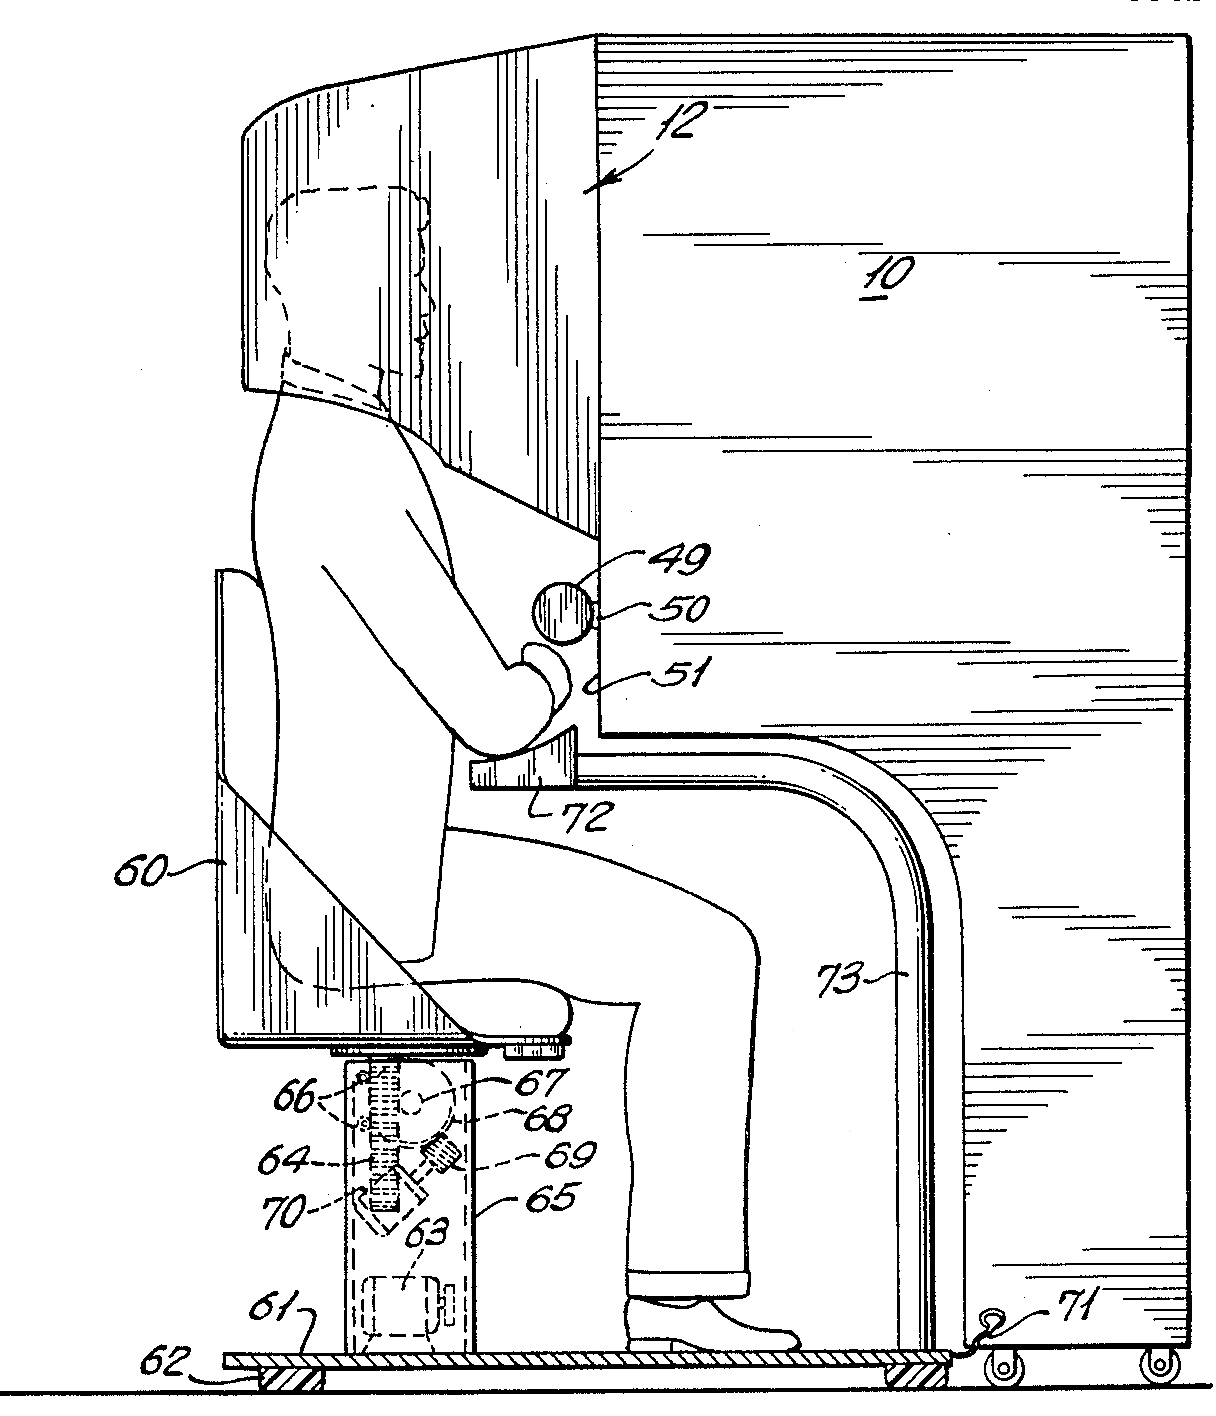
\includegraphics[scale=0.4]{senso.png}}
		\caption{Image taken from Patent filing for the Sensorama.}
		%to ref fig number
		%Figure \ref{fig:block1} shows our blockDiagram.
		\label{fig:sensorama}
	\end{figure}
	The Sensorama  was a huge box that users could stick their head into for what Hellig called the “Cinema of the future”.  It included a fully 3d display, a moving chair (coordinated with the film), and a scent creation device.  It was, perhaps predictably, a failure in terms of revolutionizing cinema, but it did inspire more experiments into virtual reality.  Many of these were military funded, the largest area of development being flight simulators, but in the consumer area the next big leap would come in 1968 with a device called the Sword of Damocles.\cite{swordDam}  It was developed by Ivan Sutherland with help from his student Bob Sproull based on a concept he came up with in 1965, and was the first VR head mounted display.  The device was incredibly bulky and had to be attached to the ceiling so as not to crush the person wearing it, and could only display rudimentary wireframes, but it was the first head mounted display and laid the foundation that our current devices have built upon.  
	\par ~\\
	Virtual reality remained mostly in labs and research facilities until 1984, when Jaron Lanier created a company called VPL research.  VPL research was one of the first companies to actually attempt to sell VR devices to the world, most notably the dataglove, a peripheral input system that used a glove as input.  This would in turn lead to Mattel creating the Powerglove in 1989, a glove based controller for the NES, one of the first attempts to sell anything virtual reality related to the mass market.  Additionally, VPL research created a more simple head mounted display called the eyephone. Jaron Lanier is also credited with coining the term “Virtual Reality” to describe such devices.  
	\subsubsection{1990-2012}
	The next big breakthrough in consumer virtual reality would come in 1990, with a company called Virtuality Group.  In 1991 they rolled out the first arcade system that relied on virtual reality, known as the 1000 series.[Fig. 2]  
		\begin{figure}[H]
			\centerline{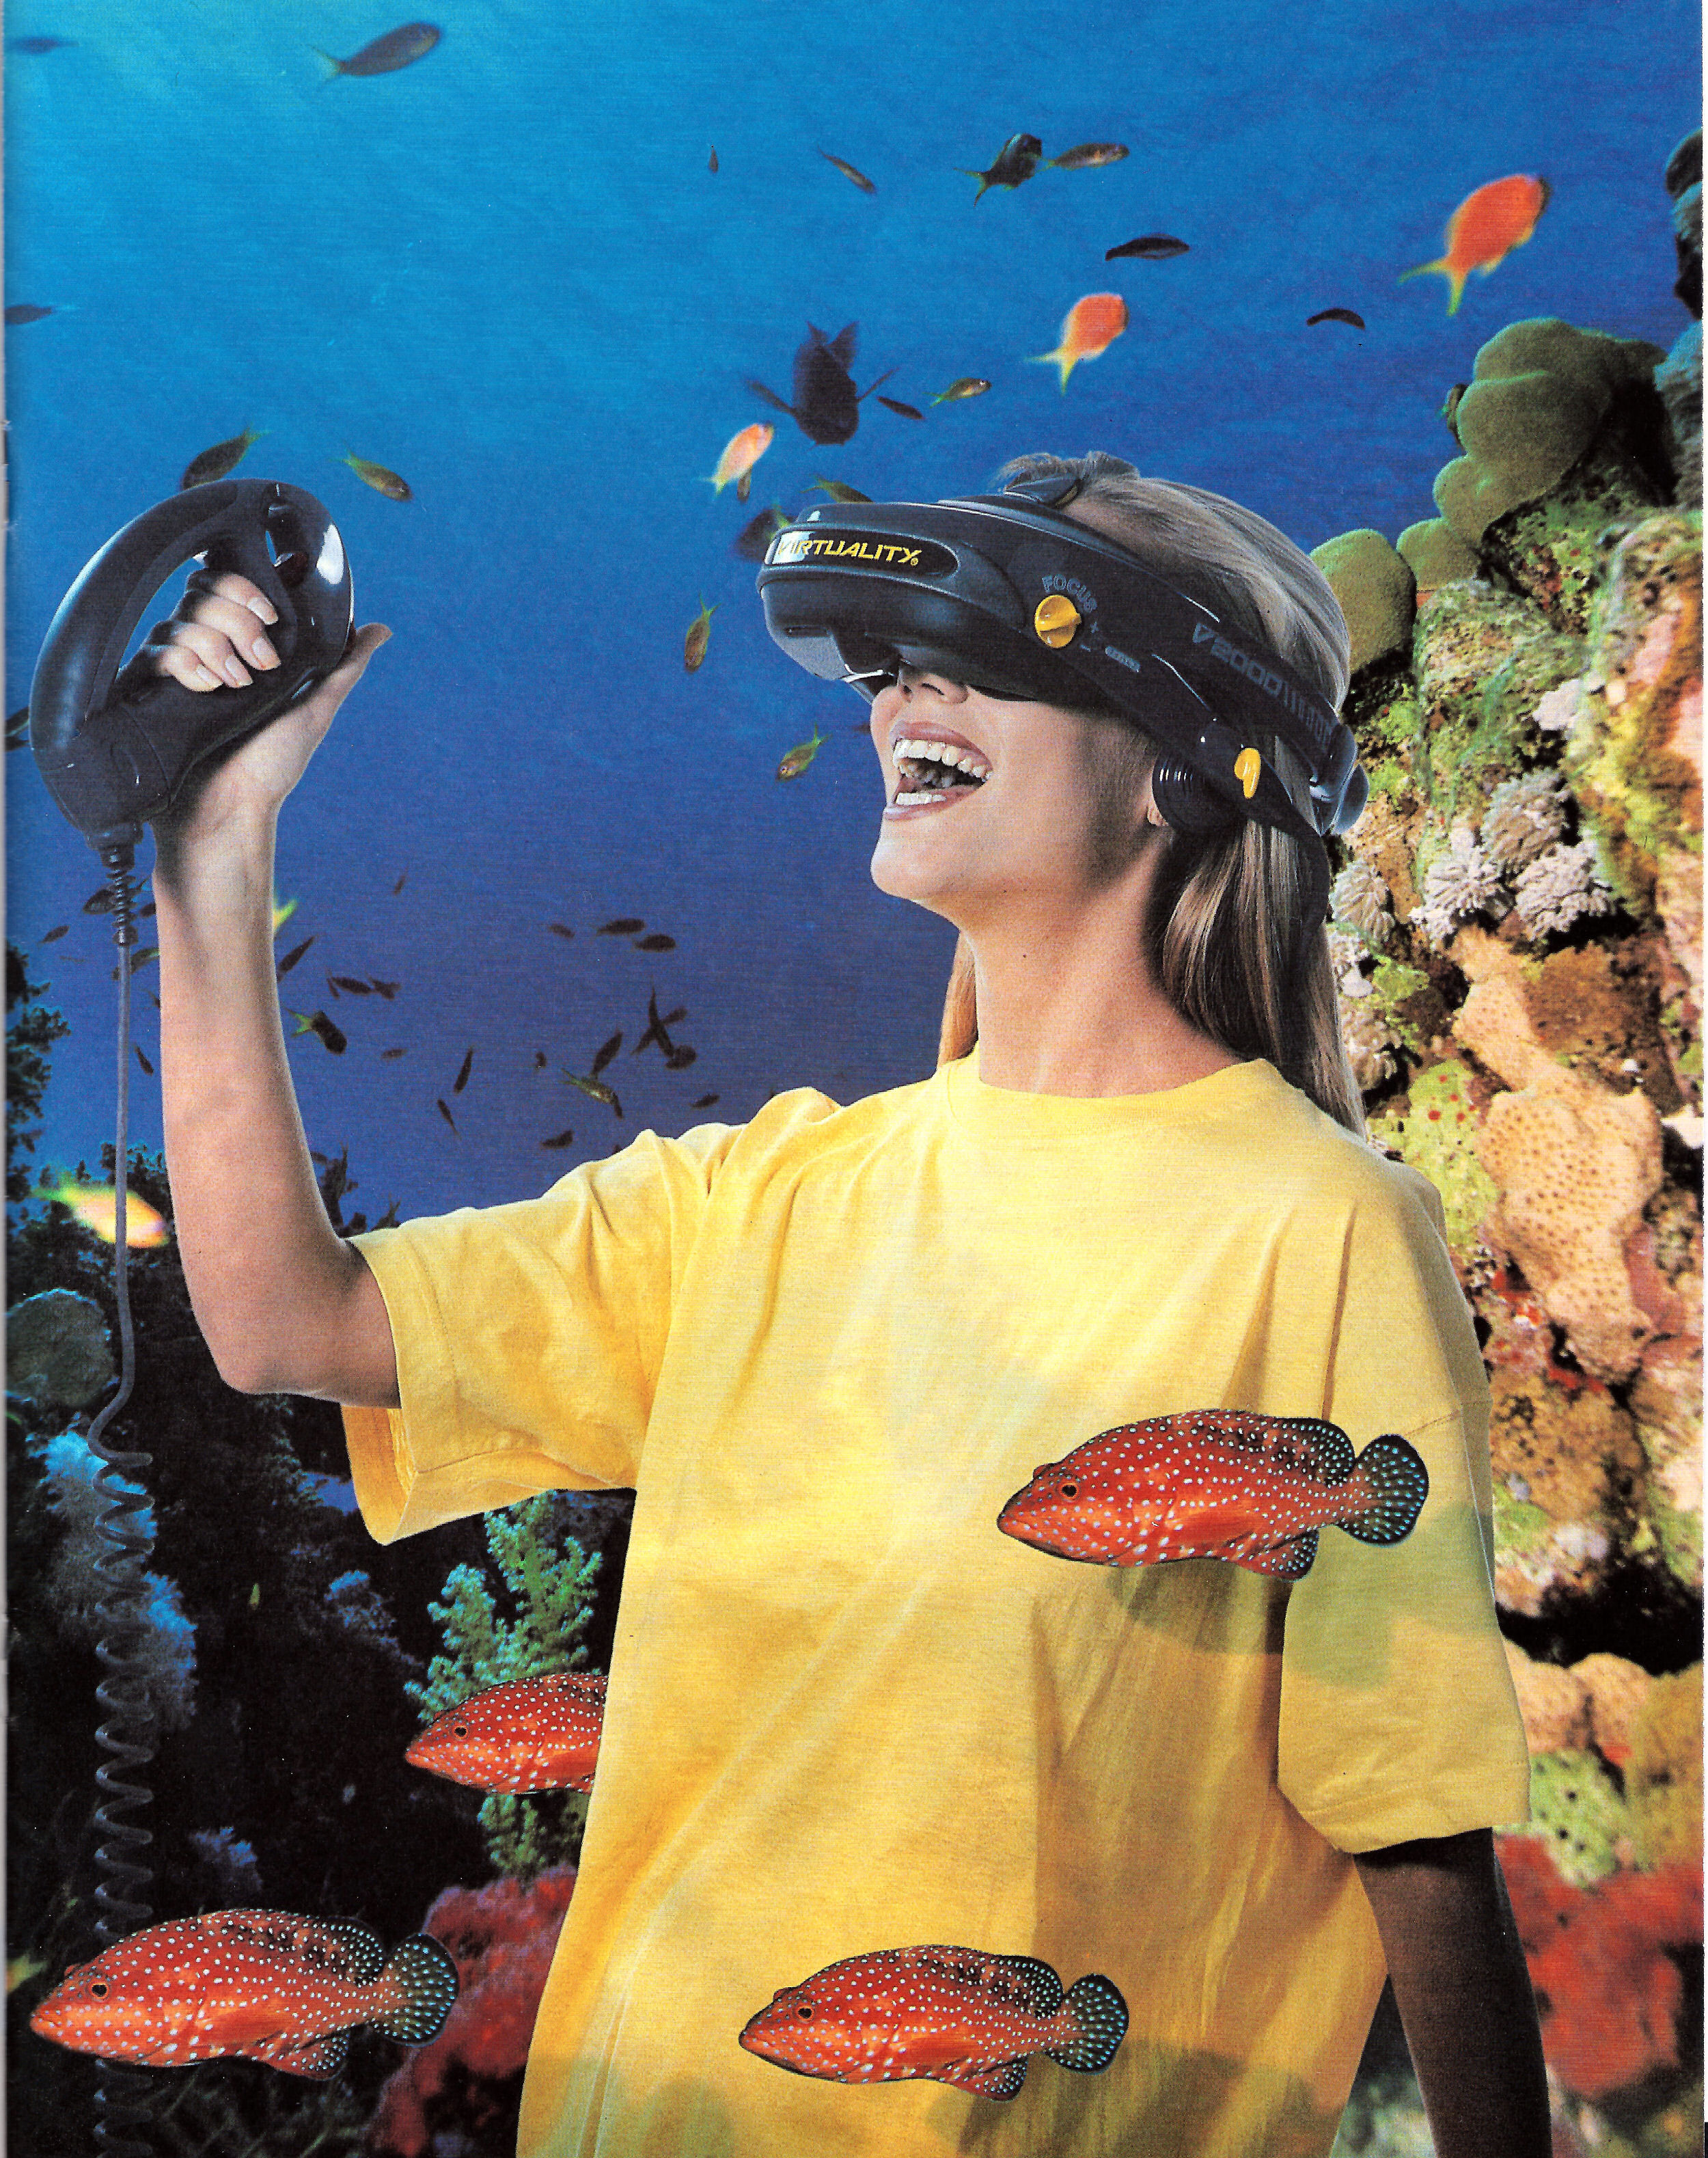
\includegraphics[scale=0.6]{virtuality.jpg}}
			\caption{Virtuality Group Advertising}
			%to ref fig number
			%Figure \ref{fig:block1} shows our blockDiagram.
			\label{fig:virtuality}
		\end{figure}It had both stand up and sit down models, all containing a headset that the user would wear.  Along with these arcade machines, Virtuality worked with Sega and Atari to create headsets for their systems, and even tried to develop their own home system.  Nintendo tried to compete as well a virtual reality console called the Virtual Boy.[Fig. 33]
	While impressive and new, all these machines were also comparatively expensive for the player, and also suffered from many of the things VR still struggles with today, like motion sickness and processing power issues.  The games that these systems created also lacked appeal as “games”, instead relying almost entirely on being an innovative new experience.  
		\par ~\\
	The VR market in the 90s turned out to be a bubble waiting to burst, and around 1995 it did.  Ben Delany (founder of Virtuality Group) also blames the internet for the death of VR in the 90s, saying “The mainstream press found other, more exciting things to talk about; especially toward the end of the ’90s when very few of the wild [VR] promises had been fulfilled. People just walked away from it.”.\cite{vergeVr}
			\par ~\\
	VR continued to be grow and be refined, but not at a consumer level.  After the failure of all the major video game companies to create a home market, the industry was declared dead by most analysts and completely ignored.  
		\par ~\\
	However, other fields of development would help create an ecosystem where the VR market could rise again.  The most obvious of these is graphical and processing power.  As computers became more and more powerful and computer graphics became more and more advanced, the idea of placing someone in a virtual world slowly became a feasible concept, as opposed to an idea that people built prototypes after.  On top of this, the huge success of the Nintendo Wii helped develop the field of Motion Controls to the point where people were prepared to consider alternate ways of interacting with a game system.  Lastly, research was still being done on ways to make Virtual Reality hardware and software more powerful.  Jaron Lanier claims that a good portion of what oculus is built on was developed by people working at USC and then posted online, as an open resource.\cite{verge}  All of these things created the platform that the Oculus Rift used as a springboard to bring back in a huge way, creating the market that we are going into.
	\subsubsection{Summation}
	
	Before the next section goes into the very recent history of VR, and it’s place in psychology fields, our project can learn some things from the more general history of VR as a consumer product.  The most important and most dangerous thing our team can learn is that our project must not rely on the novelty of virtual reality, it must stand on it’s own merits.  Relying on novelty and the “VR experience” was one of the main things that killed the VR market in 1995.  However, now is also possibly the best time in history for a project like ours, as Virtual Reality has finally hit the point where it is both as popular as it was in the 90s but also has decades of tech development behind it.  Our project is able to leverage not just public support, but years and years of study into how to create virtual worlds.  If we can successfully do that, our project should be in a very good place.
		\begin{figure}[H]
			\centerline{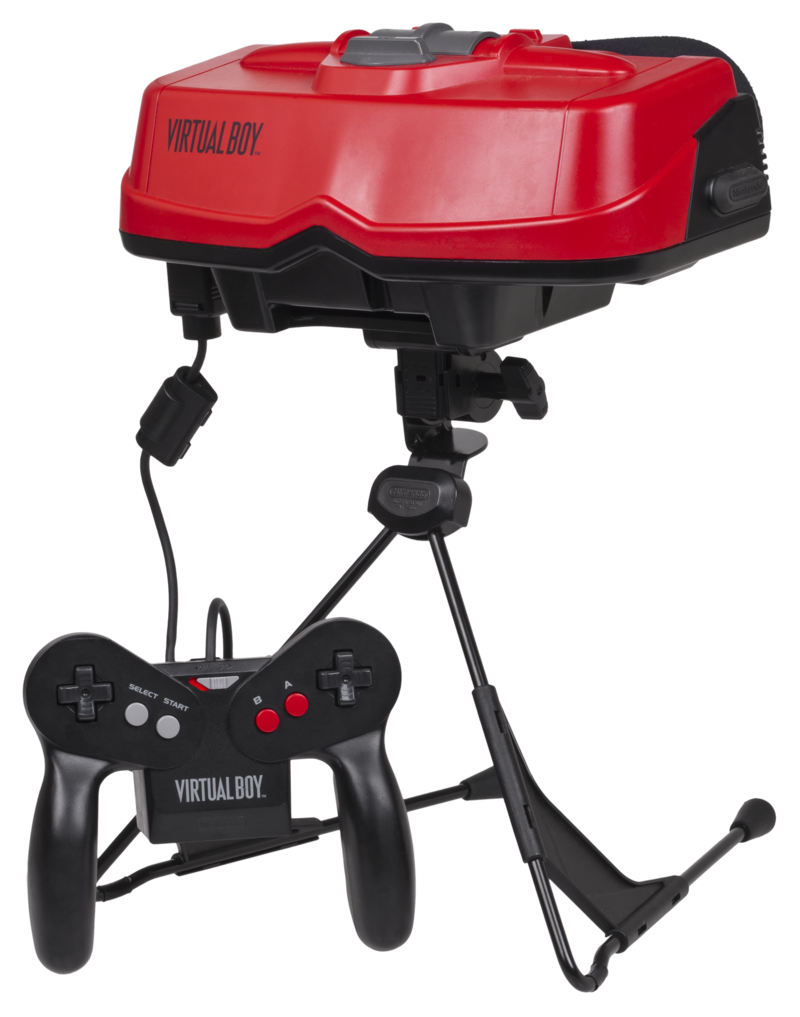
\includegraphics[scale=0.7]{virtualBoy.png}}
			\caption{Virtual Boy Advertising.}
			%to ref fig number
			%Figure \ref{fig:block1} shows our blockDiagram.
			\label{fig:vBoy}
		\end{figure}

\pagebreak

\subsection{Recent Market History}

\subsubsection{2012: Oculus Rift}

In 2012, a man named Palmer Lucky unveiled a new, consumer grade Virtual Reality device he called the Oculus Rift at the Electronic Entertainment Expo.  2 months later he started a kickstarter to try to raise funds, asking for 250,000 dollars.  This was an unprecedented resurrection of the VR market, relying on modern technology having advanced enough to actually create believable worlds and working hardware.  The project also needed to overcome the stigma that had plagued the market ever since the failure of the Virtual Boy and Virtuality.  1 month later, the project had raised a total of 2,437,429\$ breathing life into a market declared dead for over 15 years.  The kickstarter was a success beyond anyone's imaginings, and would begin a new wave of virtual reality projects.  After raising more money through venture capital and releasing a basic development prototype, om March 25, 2014 Oculus would be acquired for 2 billion dollars by Facebook.  The Virtual Reality market went from dead to 2 billion dollars in only 2 years, and suddenly a large number of companies were interested in VR.

\subsubsection{2014-Present Day: Google, HTC, Sony, and Samsung}

In 2014, 3 different companies would all announce their own attempts at a VR platform.  In March, HTC would announce it's own attempt at virtual reality, named the VIVE, in collaboration with Valve.  This collaboration is the Vive's greatest strength; it has a digital distribution platform (Steam) already at it's disposal.  
	\par ~\\
Meanwhile, Google announced a strange variation on the VR headset:  they set out plans for a headset users could make with cardboard.  The headset contained a slot to put a smartphone in, and through use of an app the user could have a Virtual Reality headset experience on any modern android equipped phone[Fig. 4].
\begin{figure}[H]
	\centerline{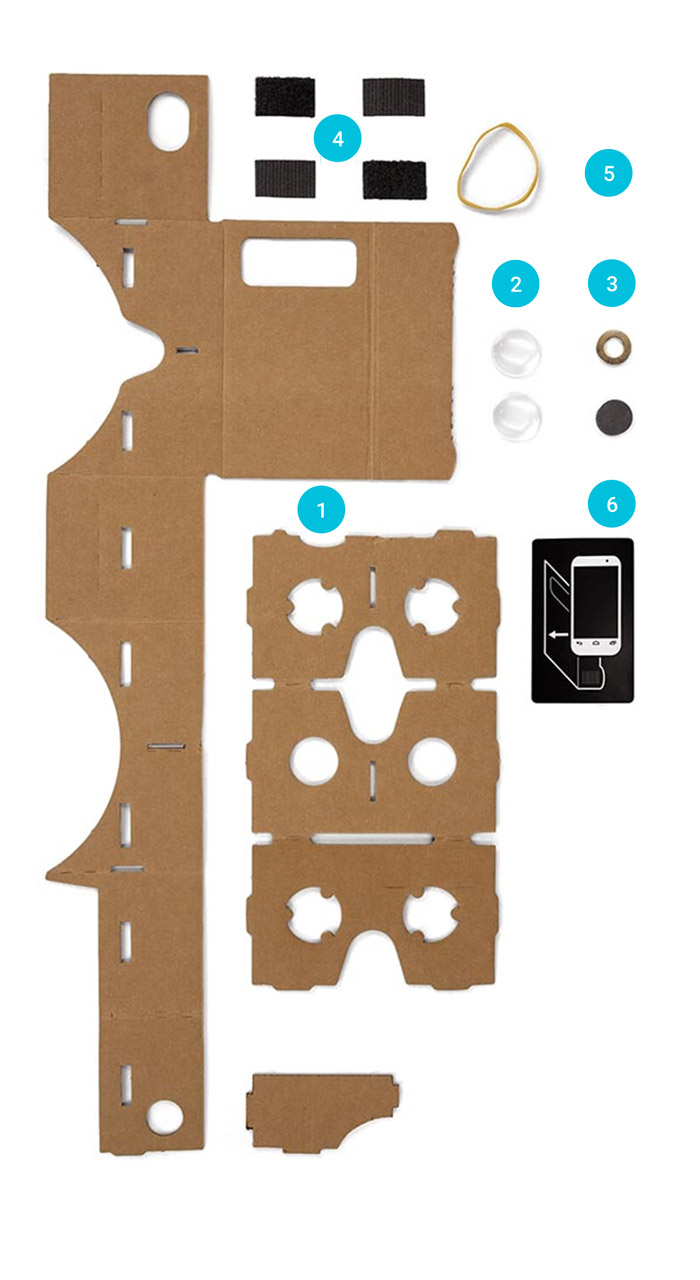
\includegraphics[scale=0.8,,keepaspectratio]{cardboard.jpg}}
	\caption{Google Cardboard}
	%to ref fig number
	%Figure \ref{fig:block1} shows our blockDiagram.
	\label{fig:cardboard}
\end{figure}
Sony would also make an announcment, unveiling the long rumored Project Morpheus at GDC.  Later it would be renamed Playstation VR, and is very heavily reliant on their playstation game console.  Most recently, Oculus announced a collaboration with Samsung to create the Samsung Gear VR.  Like the Google Cardboard, it uses a smartphone as it's display device, however it is a much more specialized device with phones built to work with VR[Fig. 5].

\begin{figure}[H]
	\centerline{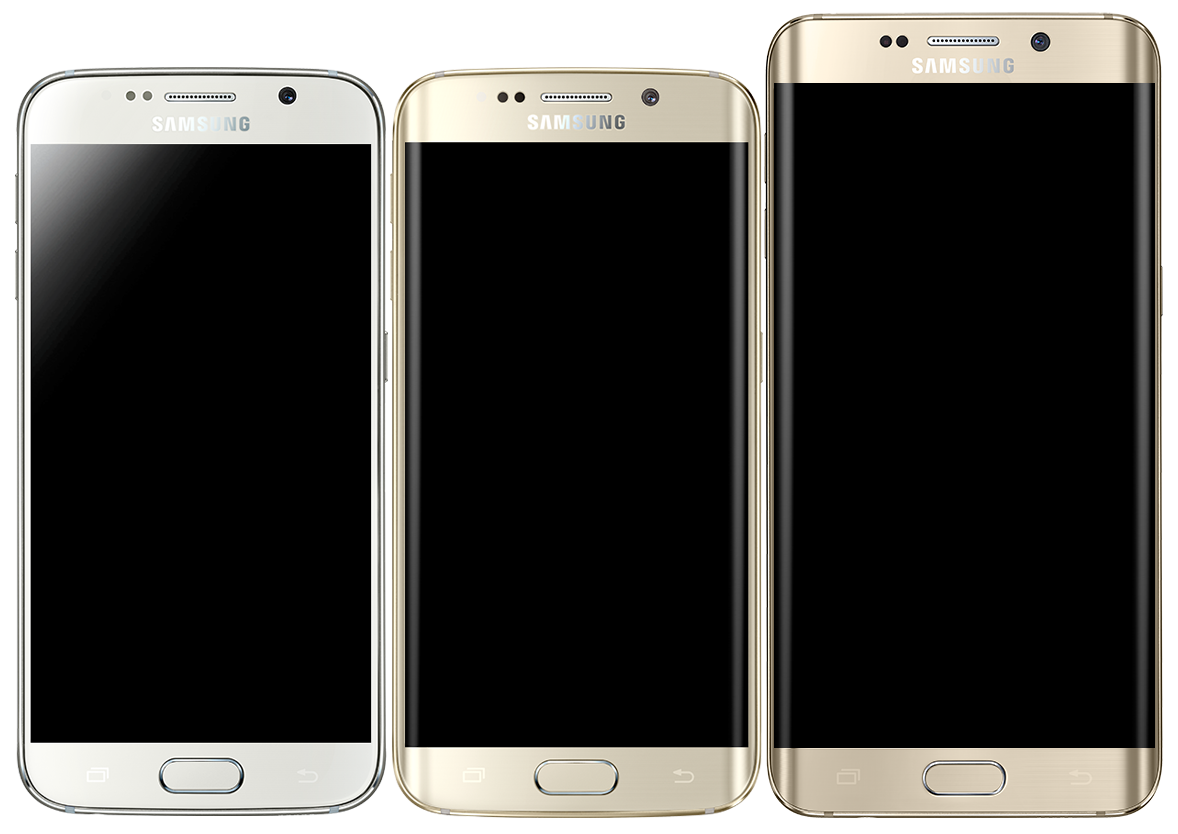
\includegraphics[width=\linewidth,height=\paperheight,keepaspectratio]{galaxy5.png}}
	\caption{Samsung Galaxy S6 series, all compatible with the Gear VR.}
	%to ref fig number
	%Figure \ref{fig:block1} shows our blockDiagram.
	\label{fig:samsungGalaxy}
\end{figure}

\subsection{Market Future}
\subsubsection{Statistics}

Current predictions for the VR market are overall positive.  The next couple of pages [Fig 6-8] are a number of statistics and surveys showing predictions for the growth of the VR field over the next 4-5 years.  Each contains a description and source.  Following this section will be a conclusion, wrapping up both the research on recent VR companies and these statistics. [Fig 6-9]

\begin{figure}[H]
	\centerline{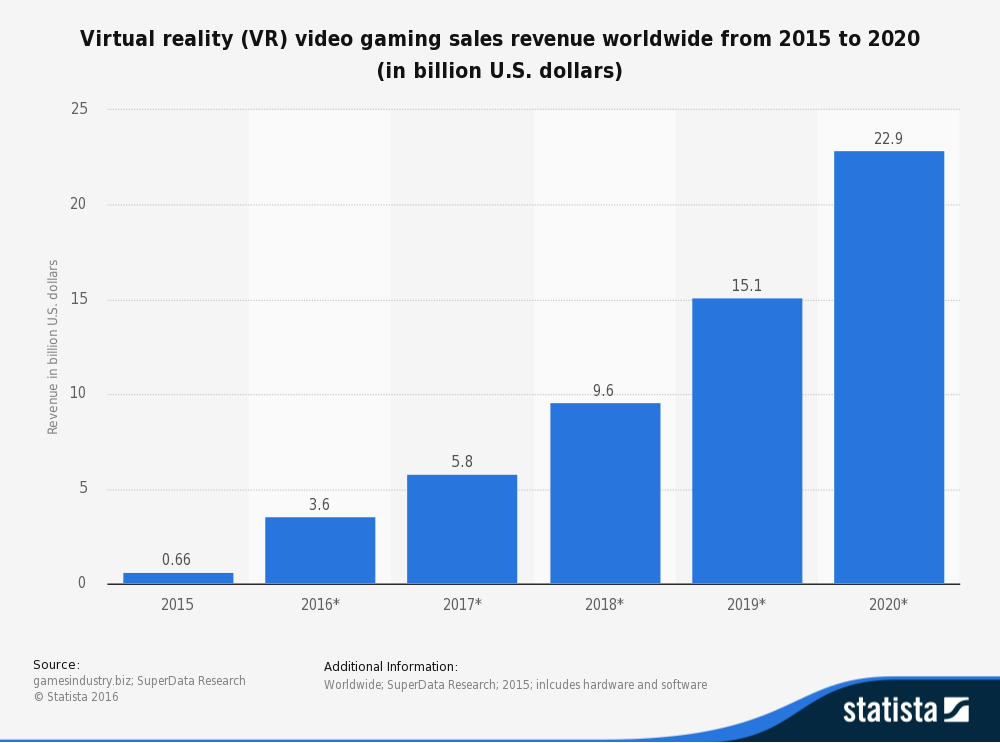
\includegraphics[scale = 0.3]{statMon2.png}}
	\caption{Prediction of the virtual reality revenue through 2020.  Obtained through Statistia.  Source: Superdata Research \cite{vrRev}}
	%to ref fig number
	%Figure \ref{fig:block1} shows our blockDiagram.
	\label{fig:virRevenue}
\end{figure}

\begin{figure}[H]
	\centerline{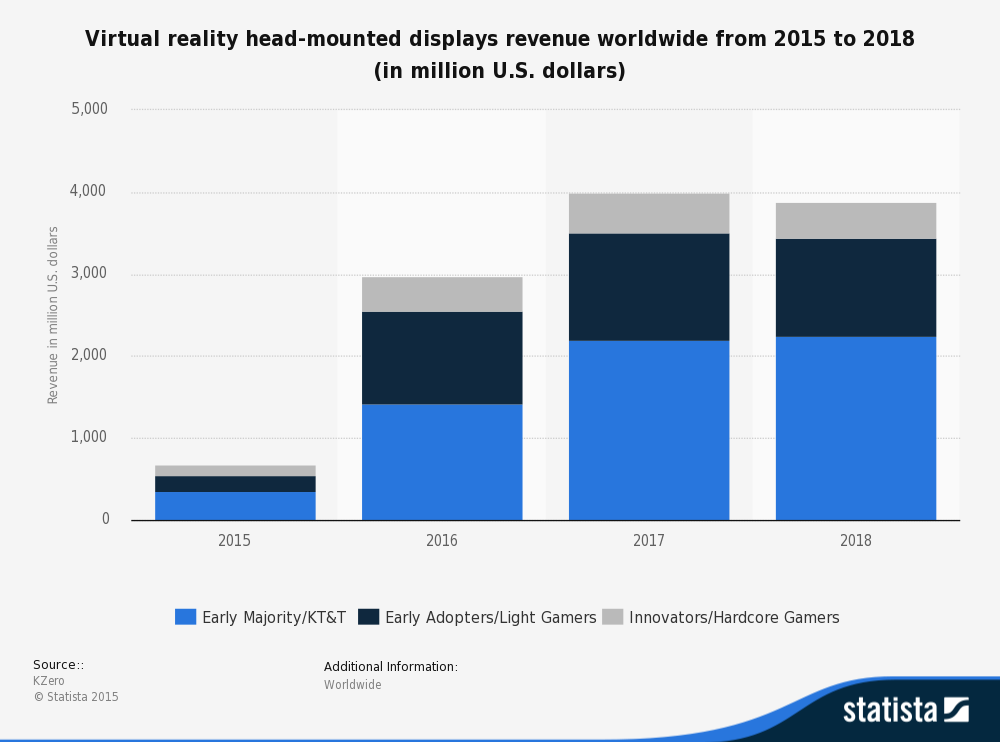
\includegraphics[scale = 0.3]{statMon.png}}
	\caption{Prediction of the Head Mounted Display Revenue through 2018.  Obtained through Statistia.  Source: KZero survey \cite{hmdRev}}
	%to ref fig number
	%Figure \ref{fig:block1} shows our blockDiagram.
	\label{fig:moneyStats}
\end{figure}

\begin{figure}[H]
	\centerline{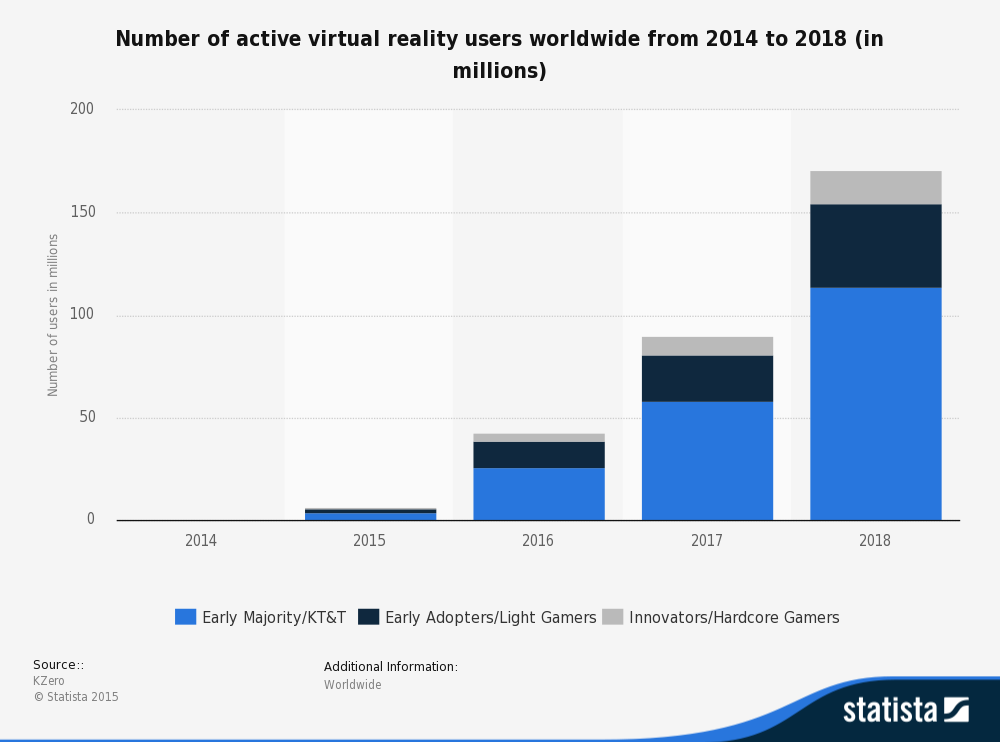
\includegraphics[scale = 0.23]{statsUsers.png}}
	\caption{Prediction of the virtual reality user acceptance through 2018.  Obtained through Statistia.  Source: KZero survey \cite{vrUser}}
	%to ref fig number
	%Figure \ref{fig:block1} shows our blockDiagram.
	\label{fig:userStats}
\end{figure}

\begin{figure}[H]
	\centerline{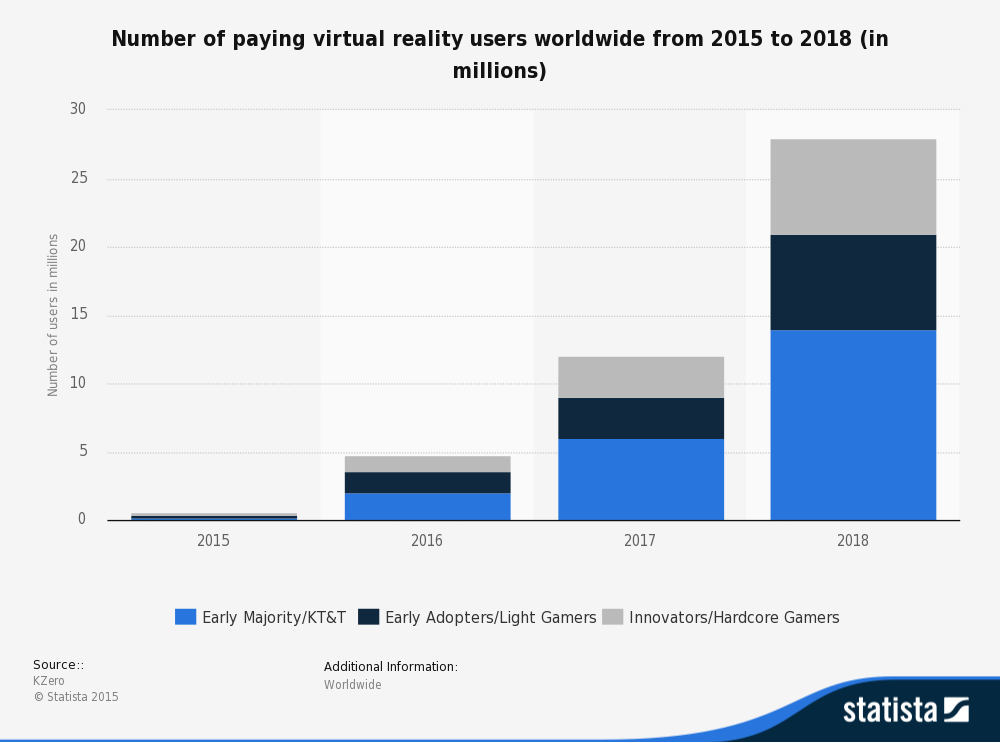
\includegraphics[scale = 0.23]{statPay.png}}
	\caption{Prediction of the paying virtual reality users through 2018.  Obtained through Statistia.  Source: KZero survey \cite{payUser}}
	%to ref fig number
	%Figure \ref{fig:block1} shows our blockDiagram.
	\label{fig:moneyStats2}
\end{figure}
\subsubsection{Conclusion}

There are two main conclusions that we can come to from this data, and the first one is cautionary.  When we look at the different VR platforms, one common theme stands out, and that is they are generally marketed as video game peripherals.  Out of the 5 devices, three of them are focused on selling video games.  Because our project shares little market space with the video game market, we may have difficulties on those platforms.  This is one reason our project will be using the Samsung Gear VR, as it is the first mass market VR headset that isn't primarily marketed as a game platform.  However, our second conclusion is more optimistic: from the statistics we found, Virtual Reality isn't predicted to slow down any time soon.  This is great news for our project as we will be entering a rapidly growing and expanding market.

\pagebreak
\subsection{VR Headset Options and Technical Capabilities}
\label{section:headset}

Following is our research on the different possible VR devices and peripherals, with information on each one.   
\subsubsection{Oculus Rift Consumer Version [Fig 10]}
\begin{itemize}
	\item Resolution: 2160 x 1200
	\item Refresh Rate: 90 Hz (11 ms )
	\item Latency: 20ms
	\item Recommended CPU: Intel i5-4590 or equivalent
	\item Recommended GPU: NVIDIA GTX 970 / AMD 290 
	\item Recommended RAM: 8GB
	\item Positional Tracking: IR Camera Sensor (5 x 11 feet)
	\item Controls: Oculus Touch (not included)
	\item Release Date: Q1 2016 (Delayed)
	\item Manufacturer: Oculus VR
	\item Unity Support: Yes
	\item OS Cross Platform: Windows and Android only. (Oculus Home Dependent)
	\item Cost: \$599
\end{itemize}
\begin{figure}[H]
	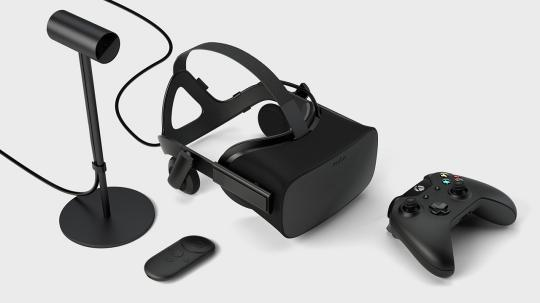
\includegraphics[width=\linewidth,height=\paperheight,keepaspectratio]{cv.jpg}
	\caption{Oculus Rift Consumer Version}
	%to ref fig number
	%Figure \ref{fig:block1} shows our blockDiagram.
	%NOTHING
	\label{fig:RiftCVImg}
	\end{figure}
	\pagebreak
\subsubsection{Oculus Rift Dev Kit 2 [Fig 11]}
\begin{itemize}
	\item Resolution: 1920 x 1080
	\item Refresh Rate: 75 Hz (13 ms)
	\item Latency: 20-40ms
	\item Recommended CPU: Intel i5-4590 or equivalent
	\item Recommended GPU: NVIDIA GTX 970 / AMD 290 
	\item Recommended RAM: 8GB
	\item Positional Tracking: IR Camera Sensor (5 x 11 feet)
	\item Controls: Oculus Touch (not included)
	\item Release Date: July 2014
	\item Manufacturer: Oculus VR
	\item OS Cross Platform: Windows and Android only. (Oculus Home Dependent)
	\item Unity Support: Yes
	\item Cost: \$350
\end{itemize}
\begin{figure}[H]
	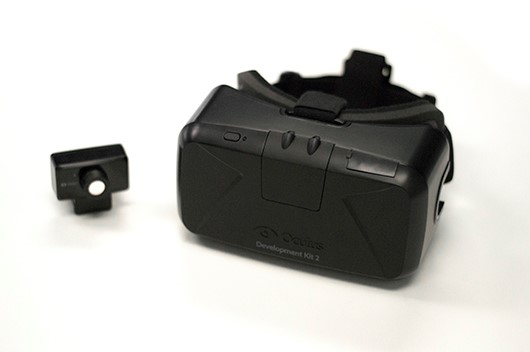
\includegraphics[width=\linewidth,height=\paperheight,keepaspectratio]{dk2.jpg}
	\caption{Oculus Rift Dev Kti 2}
	%to ref fig number
	%Figure \ref{fig:block1} shows our blockDiagram.
	\label{fig:Riftdk2Img}
	\end{figure}
	\pagebreak
\subsubsection{Oculus Rift Dev Kit 1 [Fig 12]}
\begin{itemize}
	\item Resolution: 1200 x 800
	\item Refresh Rate: 60 Hz (16 ms)
	\item Latency: 50-60ms
	\item Recommended CPU: Lower Spec (Early Prototype)
	\item Recommended GPU: Lower Spec (Early Prototype)
	\item Recommended RAM: 4GB
	\item Positional Tracking: No
	\item Controls: Oculus Touch (not included) 
	\item Release Date: August 2012 (Kickstarter)
	\item Manufacturer: Oculus VR
	\item Cross Platform: Windows and Android only. (Oculus Home Dependent)
	\item Unity Support: Yes
	\item Cost: \$300
\end{itemize}
	\begin{figure}[H]
	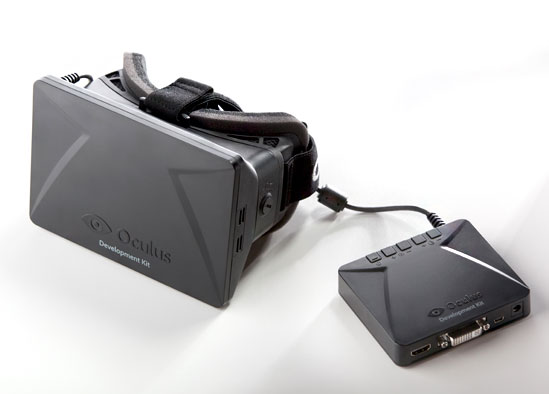
\includegraphics[width=\linewidth,height=\paperheight,keepaspectratio]{dk1.jpg}
	\caption{Oculus Rift Dev Kit 1}
	%to ref fig number
	%Figure \ref{fig:block1} shows our blockDiagram.
	\label{fig:Riftdk1Img}
	\end{figure}
	\pagebreak
\subsubsection{Samsung Gear VR [Fig 13]}
\label{section:gearVR}
	Supported phones include the Samsung Galaxy: Note5, S6, S6 edge, S7, S7 edge  
	\begin{itemize}
	  \item Resolution: 2560 X 1440 (Quad HD phone screen)
	  \item Refresh Rate: 60 Hz (16 ms)
	  \item Latency: 50-60ms
	  \item Recommended CPU: Phone Dependent
	  \item Recommended GPU: Phone Dependent
	  \item Recommended RAM: Phone Dependent
	  \item Positional Tracking: No
	  \item Controls: Touch pad, back button, volume controls
	  \item Release Date: November 2015
	  \item Manufacturer: Samsung, With technology by Oculus VR
	  \item Cross Platform: Windows and Android only. (Oculus Home Dependent)
	  \item Unity Support: Yes
	  \item Cost: \$99
	\end{itemize}
	\begin{figure}[H]
	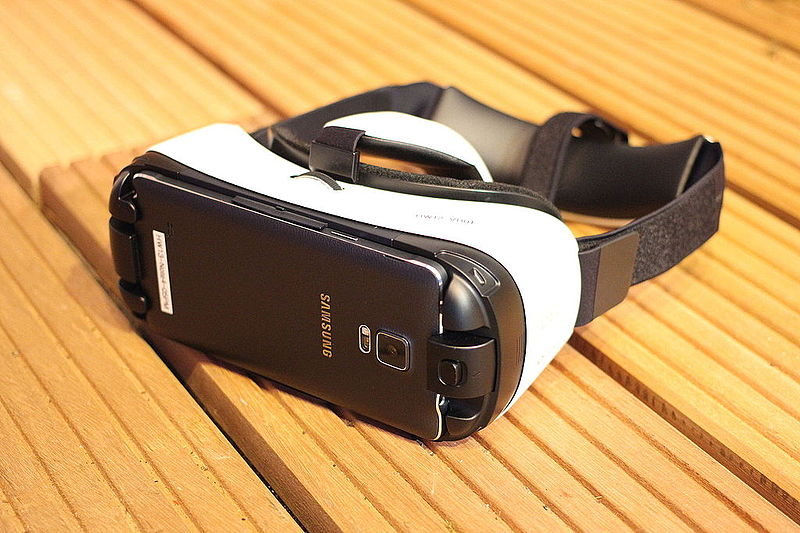
\includegraphics[width=\linewidth,height=\paperheight,keepaspectratio]{gear.jpg}
	\caption{Samsung Gear VR}
	%to ref fig number
	%Figure \ref{fig:block1} shows our blockDiagram.
	\label{fig:GearImg}
	\end{figure}
	\pagebreak
\subsubsection{HTC Vive [Fig 14]}
	\begin{itemize}
	  \item Resolution: 2160 x 1200
	  \item Refresh Rate: 90 Hz (11 ms)
	  \item Latency: 22ms
	  \item Recommended CPU: Intel i5-4590 or equivalent
	  \item Recommended GPU: NVIDIA GTX 970 / AMD 280 
	  \item Recommended RAM: 4GB
	  \item Positional Tracking: IR Camera Sensor (15 x 15 feet)
	  \item Controls: Motion Controllers (included) (similar to Occulus Touch)  
	  \item Release Date: Q1 2016 (Delayed)
	  \item Manufacturer: HTC, With technology by Valve Corporation
	  \item Cross Platfrom: Valve OpenGL Mesa support/ SteamVR support on Linux soon hopefully
	  \item Unity Support: Yes
	  \item Cost: \$799
	\end{itemize}
	\begin{figure}[H]
	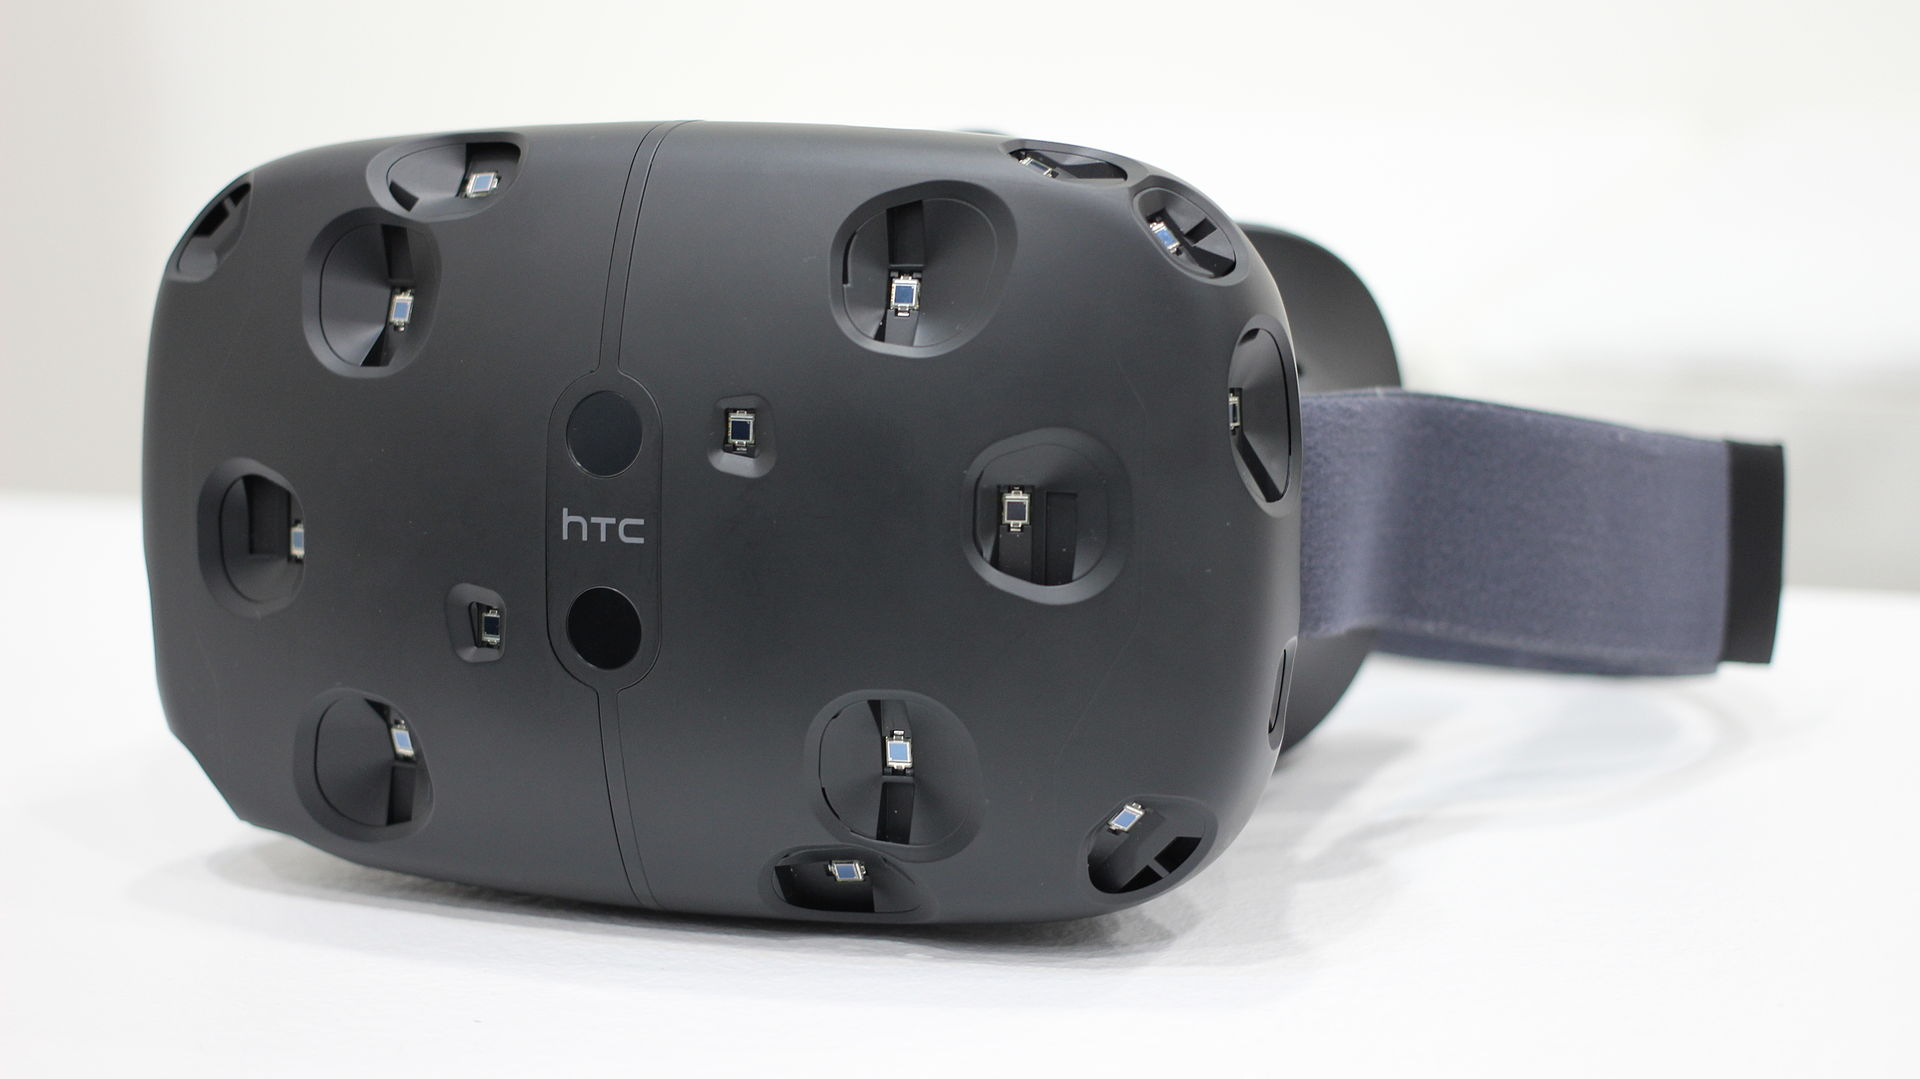
\includegraphics[width=\linewidth,height=\paperheight,keepaspectratio]{vive.jpg}
	\caption{HTC Vive Headset}
	%to ref fig number
	%Figure \ref{fig:block1} shows our blockDiagram.
	\label{fig:ViveImg}
	\end{figure}
	\pagebreak
\subsubsection{PS4 Morpheus [Fig 15]}
\begin{itemize}
  \item Resolution: 3840 x 1080 
  \item Refresh Rate: 120 Hz (8 ms)
  \item Latency: 18ms
  \item Recommended CPU: PS4
  \item Recommended GPU: PS4
  \item Recommended RAM: PS4
  \item Positional Tracking: Playstation Camera area ~(18 x 12 feet)
  \item Controls: Playstation Move Controllers (not included)
  \item Release Date: Q1 2016 (Delayed)
  \item Manufacturer: Sony
  \item Cross Platfrom: No
    \item Unity Support: Yes
  \item Unity Support: Yes
  \item Cost: \$399
\end{itemize}
\begin{figure}[H]
	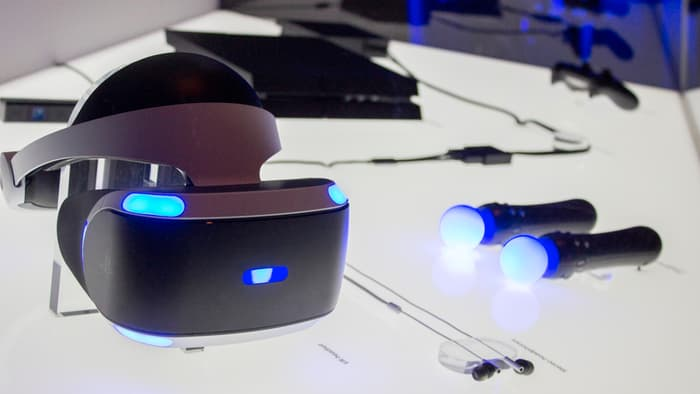
\includegraphics[width=\linewidth,height=\paperheight,keepaspectratio]{morpheus.jpg}
	\caption{Playstation VR}
	%to ref fig number
	%Figure \ref{fig:block1} shows our blockDiagram.
	\label{fig:psvrImg}
\end{figure}
	\pagebreak
	
\pagebreak
\subsection{VR Peripheral Options}
\label{section:peripheral}
\subsubsection{Leap Motion [Fig 16]}
\begin{itemize}
	\item Using Leap Motion on a PC is viable in Unity and very well supported, however using Leap Motion and the Gear VR simultaneously on Android is not feasible, this is due to the high level of processing required to
	handle the areas tracked by the leap sensor. 
	\item The primary support is designed to work with the Oculus rift, and unity is supported by the Leap SDK. Making it a powerful useful sensor for hand tracking. The 
	Leap motion is supported on the Oculus DK2 and the new CV (consumer release). 
\end{itemize}
\begin{figure}[H]
	\centerline{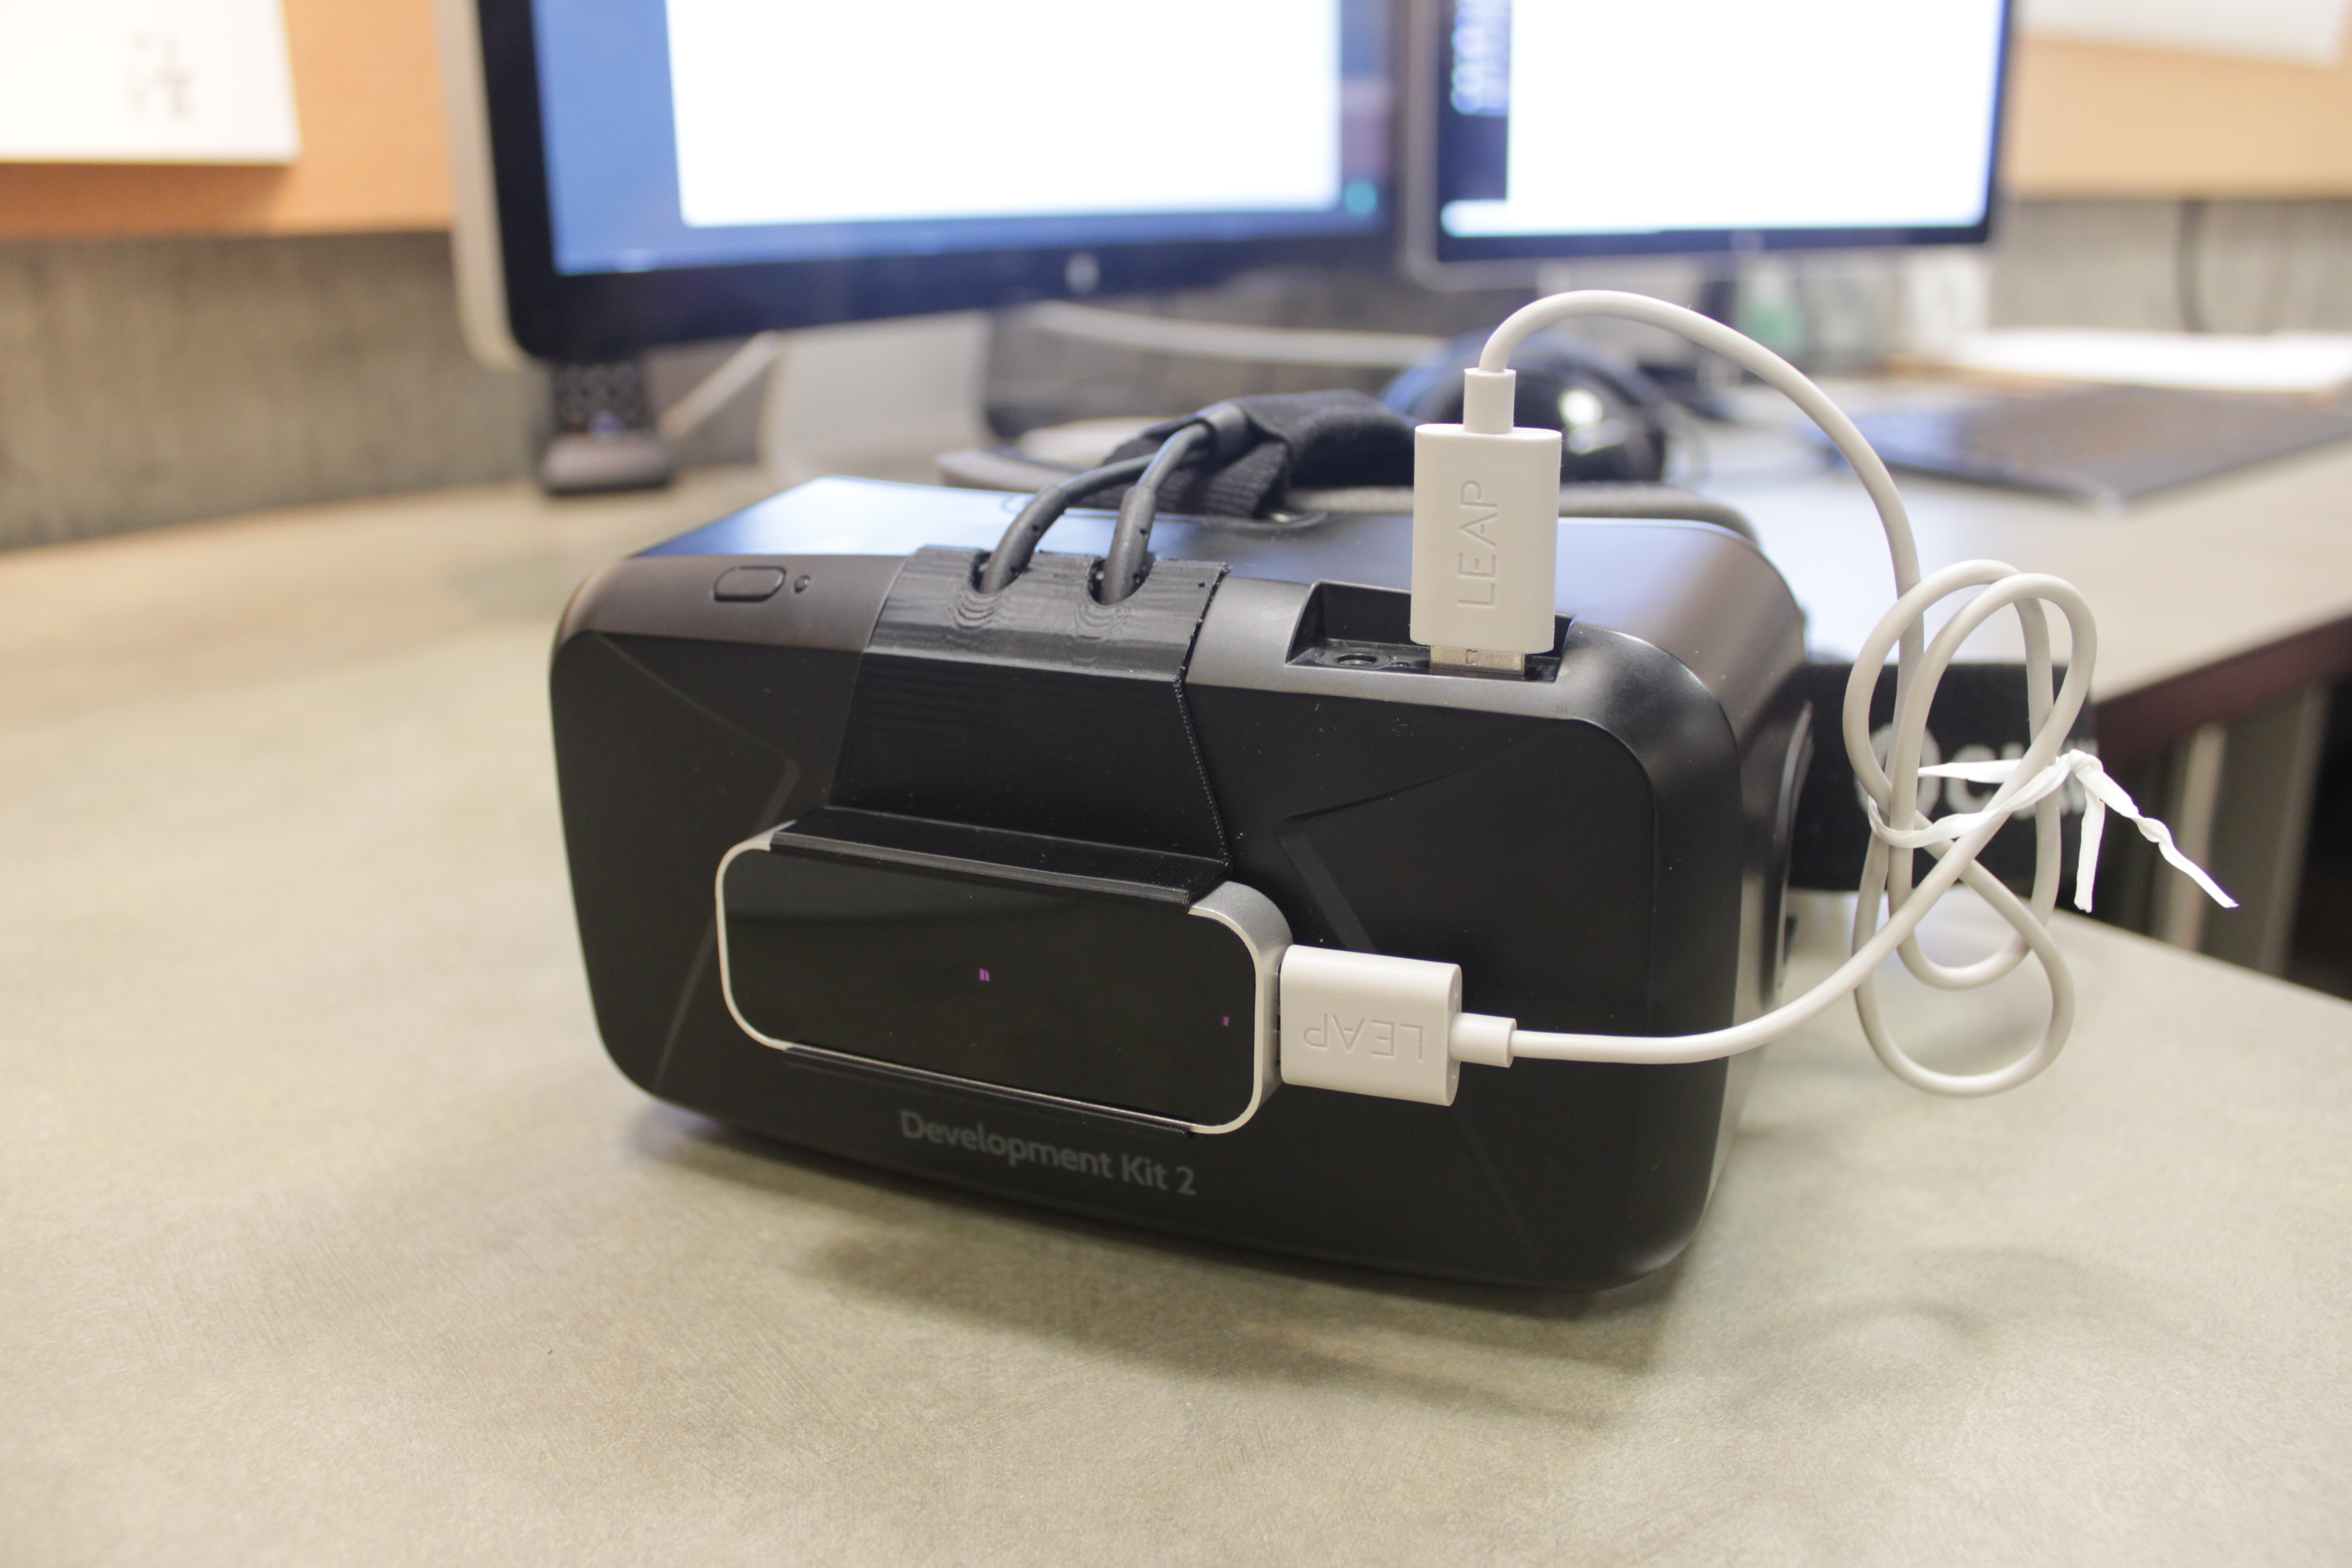
\includegraphics[scale= 0.13]{leap.jpg}}
	\caption{Leap Motion}
	%to ref fig number
	%Figure \ref{fig:block1} shows our blockDiagram.
	\label{fig:leapImg}
\end{figure}
	%leap motion research
	
\subsubsection{Red Samurai Bluetooth Controller}
	A cheap, \$8 bluetooth controller, that pairs very well with the Gear VR on Android, this would be allow the user to move around the scene as we would be unable to get the other Peripherals to work with the phone.
	
\subsubsection{Oculus Head Tracking Research}
The following information is from the Oculus Rift prototype research paper see the it for more details on the math behind their calculations \cite{riftPaper}~\\
All sensing is performed by a single circuit board (figure \ref{fig:magnetsHowDoTheyWork}) 
\begin{itemize}
\item The main components [Fig 17] are:
\begin{itemize}
 \item STMicroelectronics 32F103C8 ARM Cortex-M3 microcontroller
 \item Invensense MPU-6000 (gyroscope + accelerometer)
 \item Honeywell HMC5983 magnetometer.
\end{itemize}
\begin{figure}[H]
	\centerline{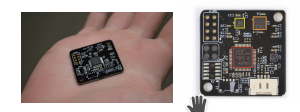
\includegraphics[]{riftMagnets.png}}
	\caption{Rift Head tracking sensor}
	%to ref fig number
	%Figure \ref{fig:block1} shows our blockDiagram.
	\label{fig:magnetsHowDoTheyWork}
	\end{figure}
	

\item The microcontroller interfaces between the sensor chips
and the PC over USB. The gyroscope, accelerometer, and magnetometer provide three-axis measurements.

\item Sensor observations are reported at a rate of 1000Hz.
\item The following measurements are calculated from these sensors.
  \begin{enumerate}
  \item Angular velocity (rad/sec)
  \item Linear acceleration (m/s2)
  \item Magnetic field strength (B Gauss)
  \end{enumerate}
\end{itemize}
% http://msl.cs.uiuc.edu/~lavalle/papers/LavYerKatAnt14.pdf
These measurements are used to calcaulate the following:
By Euler’s Rotation Theorem, any 3D orientation can
be produced by a single rotation about one particular axis
through the origin. This representation maps to the following Coordiante system [Fig 18]:
 \begin{figure}[H]
	\centerline{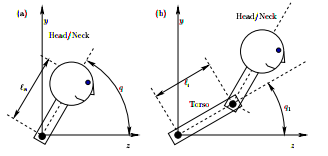
\includegraphics[scale=0.7]{riftHead.png}}
	\caption{Rift Head Coordinate System}
	%to ref fig number
	%Figure \ref{fig:block1} shows our blockDiagram.
	\label{fig:magnets2}
	\end{figure}
 \pagebreak
\subsubsection{Leap Motion Hand Tracking}
The Leap Motion works using the following sensors and lights \cite{leapProc}
\begin{itemize}
 \item Wide angle lenses give the Leap a maximum detection area of eight cubic feet, the intersection of the binocular cameras’ fields of view. 
 \item The software recognized viewing range is 2 ft (60 cm) for the standard drivers and 2.6 feet (80 cm) with the Orion Beta Driver. 
 \item The LED light that is used in detection is the limiting factor as the brightness intensity is limited by the amount of power delivered to the unit
 over USB.
 \item The 3 USB lights emit at a wavelength of 850 nanometers, outside the visible light spectrum.
\end{itemize}

The Leap Motion SDK offers the following heuristics for assisting with the tracking problem.\cite{leapHeuristics}
\begin{itemize}
 \item Tracking consistency:  The API offers a diagnostic visualizer, and a tracking confidence level.
 \item Ease of detection: This is related to how well defined certain motions are. 
 \item Occlusion: Accounting for blockage of the tracked hand by other objects, the Orion beta driver has made some improvements with this issue.
 \item All of these features show the advanced design of the sensor, and many of the innovations Leap Motion has brought to the field of virtual reality. 
\end{itemize}

This graph [Fig 19] shows the advanced tracking capabilities of the system as a possible state transition of user movement inputs.
 \begin{figure}[H]
\centerline{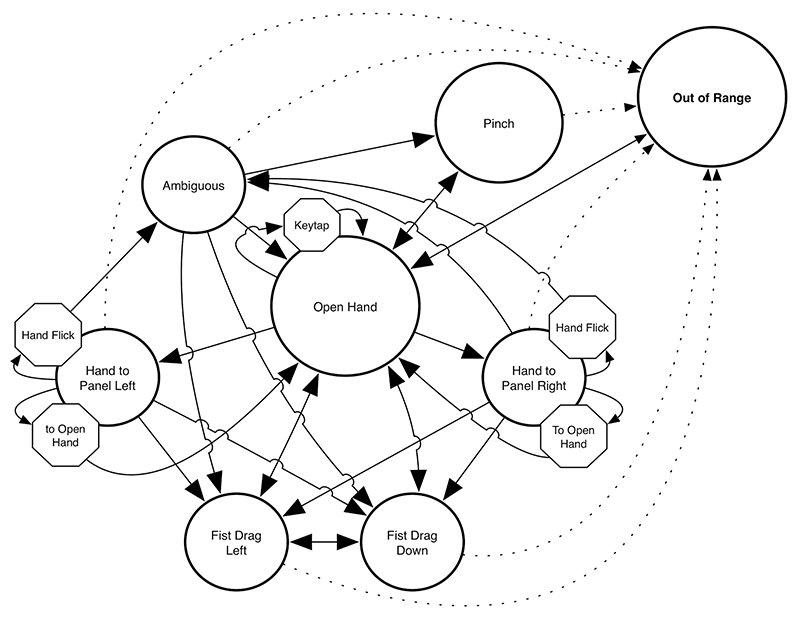
\includegraphics[scale=0.4]{leapGraph.png}}
	\caption{Leap Motion gesture graph}
	%to ref fig number
	%Figure \ref{fig:block1} shows our blockDiagram.
	\label{fig:handGraph}
	\end{figure}
\subsection{Movement Tracking Cameras}
\subsubsection{Microsoft Kinect 1 [Fig 20]}
\begin{itemize}
  \item Resolution: 640 X 480
  \item Refresh Rate: 33 Hz (30 FPS)
  \item Max Depth: 12 feet
  \item Release Date: August 2010 
  \item Manufacturer: Microsoft
  \item Cross Platform: Yes
  \item Unity Support: Yes
  \item Skeleton Joints:: 26
  \item Horizontal FOV: 57 Degrees
  \item Vertical FOV: 43 Degrees
  \item Pixels Per Degree: 5 X 5
  \item Technique: Structured Light Patterns
  \item Cost: Acquired, Not widely available, ~\$40
\end{itemize}
\begin{figure}[H]
	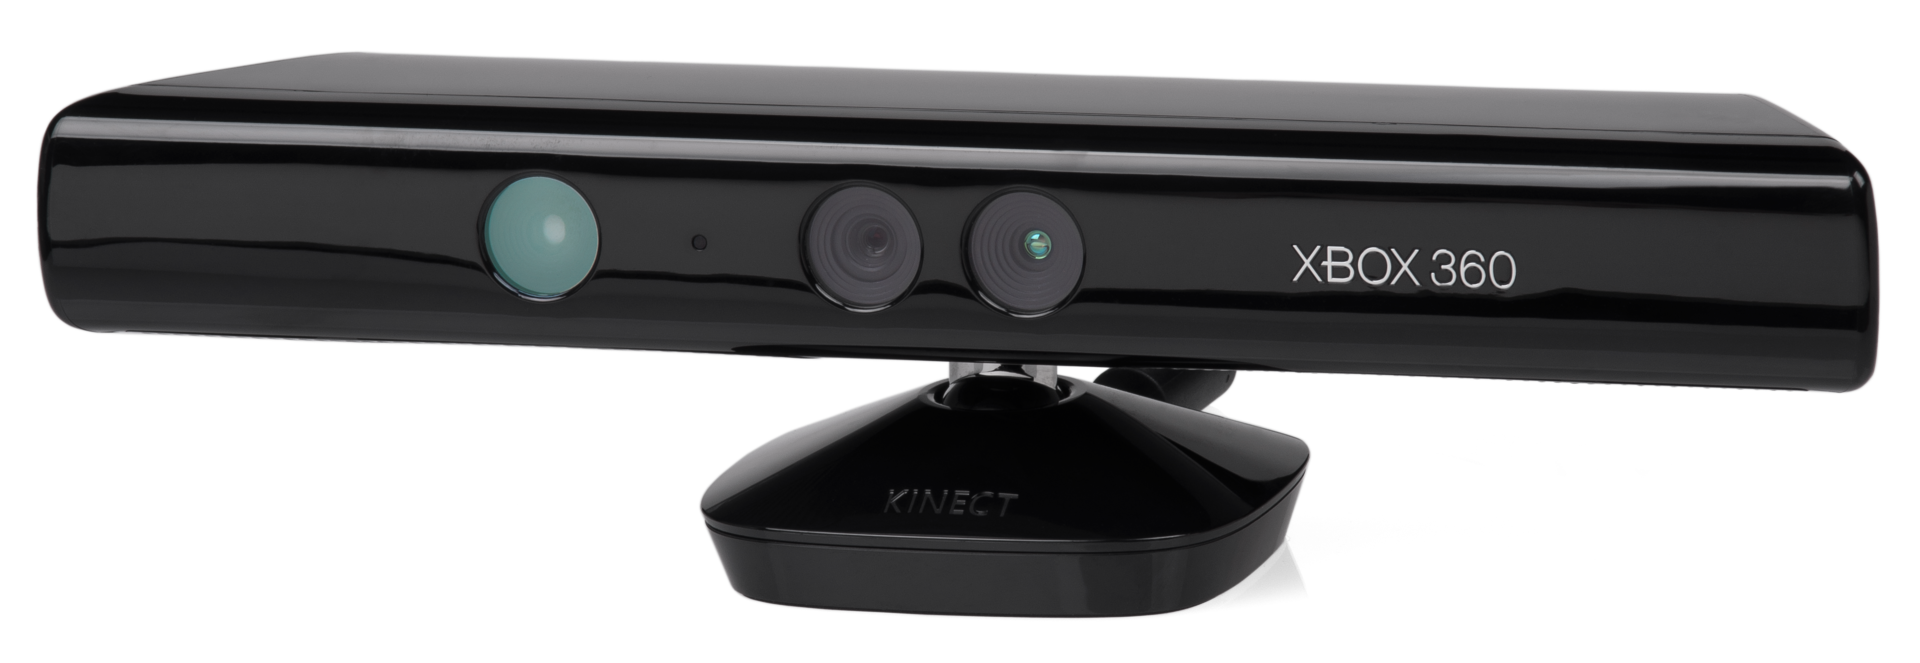
\includegraphics[width=\linewidth,height=\paperheight,keepaspectratio]{kinect1.png}
	\caption{Kinect 1 Camera, Public Domain}
	%to ref fig number
	%Figure \ref{fig:block1} shows our blockDiagram.
	\label{fig:k1Cam}
	\end{figure}
	\pagebreak
	\subsubsection{Microsoft Kinect 2 [Fig 21]}
\begin{itemize}
  \item Resolution: 1920 X 1080
  \item Refresh Rate: 33 Hz (30 FPS)
  \item Max Depth: 12 feet
  \item Release Date: August 2010 
  \item Manufacturer: Microsoft
  \item Cross Platform: Yes
  \item Skeleton Joints: 26
  \item Horizontal FOV: 70 Degrees
  \item Vertical FOV: 60 Degrees
  \item Pixels Per Degree: 7 X 7
  \item Technique: Time of Flight
  \item Cost: \$99
\end{itemize}
\begin{figure}[H]
	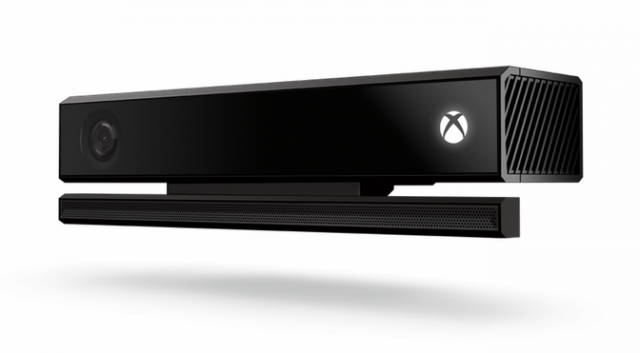
\includegraphics[width=\linewidth,height=\paperheight,keepaspectratio]{kinect2.jpg}
	\caption{Kinect 2 Camera, Public Domain}
	%to ref fig number
	%Figure \ref{fig:block1} shows our blockDiagram.
	\label{fig:k2Cam}
	\end{figure}
	\pagebreak
	
\subsubsection{Comparison of Kinect Systems}
\textbf{[Figure \ref{fig:kimg}]} Shows the increased fidelity and quality of the captured image on the Kinect 2.
\begin{figure}[H]
	\centerline{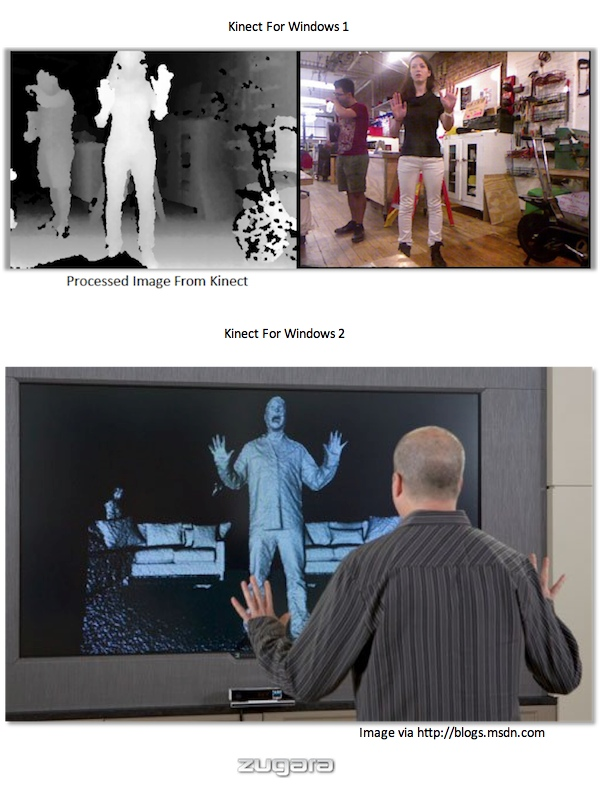
\includegraphics[scale=0.4]{kinectImg.jpg}}
	\caption{Kinect 2 Camera}
	%to ref fig number
	%Figure \ref{fig:block1} shows our blockDiagram.
	\label{fig:kimg}
	\end{figure}
	For our project we will use the Kinect for user body and movement tracking. The kinect version 1 and 2 (for the Xbox 360/ Xbox one) are both powerful devices that have many 
	advanced Capabilities (see the beginning of this subsection for more specific details). Both devices work with Unity and the SDK and Documentation show many uses including gesture 
	recognition, body tracking, head scanning, and user modeling.
	\pagebreak	
\subsubsection{Kinect Coordiante Mapping System}
The follow information and figures are from the Microsoft Kinect SDK Documentation \cite{msdnKinect}
\paragraph{Data Capture}
\begin{itemize}
\item A Kinect streams out color, depth, and skeleton data one frame at a time. [Fig 23] 
\begin{figure}[H]
	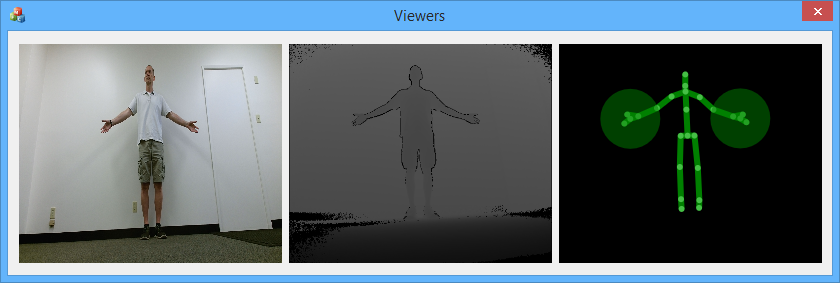
\includegraphics[width=\linewidth,height=\paperheight,keepaspectratio]{kinectCoord.png}
	\caption{GPU Architecture Diagram}
	%Figure \ref{fig:gpgpuImg} shows our blockDiagram.
	\label{fig:kinectCoord}
	\end{figure}

\item Each frame, the color sensor captures an image of everything it sees. The number of pixels depends on the device. Each pixel contains the RGB value of a particular location.

\item Each frame, the depth sensor captures a grayscale image of everything it sees. Each pixel contains the Cartesian distance, in millimeters, from the camera plane to the nearest 
object at that particular (x, y) coordinate.

\item The depth sensor has two depth ranges: the default range and the near range The default range is available for both the Kinect 1 and 2 the near range is available only for the Kinect 2. [Fig 24]
\begin{figure}[H] %https://msdn.microsoft.com/en-us/library/hh973078.aspx#Depth_Ranges
	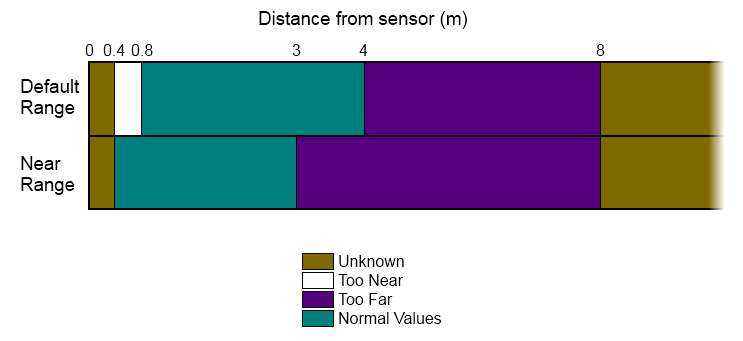
\includegraphics[width=\linewidth,height=\paperheight,keepaspectratio]{kinectRange.png}
	\caption{GPU Architecture Diagram}
	%Figure \ref{fig:gpgpuImg} shows our blockDiagram.
	\label{fig:kinectRange}
	\end{figure}
\item Each frame, the depth image captured is processed by the Kinect runtime into skeleton data. Skeleton data contains 3D position data for human skeletons for up to two people who
are visible in the depth sensor. The position of a skeleton and each of the skeleton joints (if active tracking is enabled) are stored as (x, y, z) coordinates.

	%http://files.channel9.msdn.com/wlwimages/f1dda9cc6de74512b7c19f0101402403/image%5B11%5D-43.png
\end{itemize}
	
\paragraph{Floor Determination}
\begin{itemize}
 
\item Each skeleton frame also contains a floor-clipping-plane vector, which contains the coefficients of an estimated floor-plane equation. It is used as a clipping plane for
removing the background and segmenting players.
\item \textbf{The general plane equation is:}
\begin{equation}
  Ax + By + Cz + D = 0 
\end{equation}
 \textit{Where A,B,C,D are the coordinates of the floor clip points.}~\\
The plane equation is normalized so that the physical interpretation of D is the height of the camera from the floor, if the floor is not detectable 
the plane is the zero vector.

\end{itemize}
\paragraph{User Interaction Area} 
The interaction space is the area in front of the infrared and color sensors. The Kinect is often placed at the level of a user's head.
To increase the possible interaction space, the Kinect can tilt +27 and -27 degrees, which greatly increases the size of the interaction area. \textbf{[see figure \ref{fig:kinectFov}]}
\begin{figure}[H] %https://msdn.microsoft.com/en-us/library/hh973078.aspx#Depth_Ranges
	\centerline {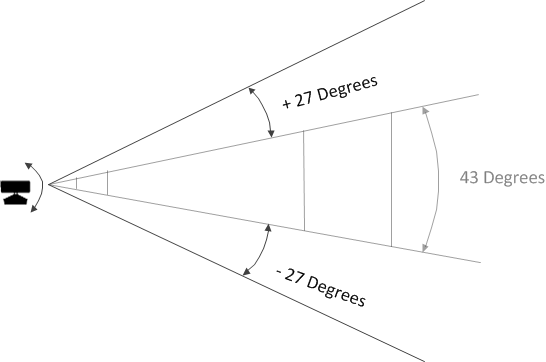
\includegraphics[scale = 0.75]{kinectFov.png}}
	\caption{Kinect FOV Digram}
	%Figure \ref{fig:gpgpuImg} shows our blockDiagram.
	\label{fig:kinectFov}
	\end{figure}
\pagebreak



	
\subsubsection{Oculus Rift DK2+ Camera}
\begin{itemize}
  \item Resolution: 752×480
  \item Refresh Rate: 16 Hz (60 FPS)
  \item Max Depth: ?
  \item Release Date: July 2014
  \item Manufacturer: Oculus Rift
  \item Cross Platform: No
  \item Skeleton Joints: Headset Position
  \item Technique: IR LED Pattern Recognition
  \item Cost: Included With Headset
\end{itemize}
\begin{figure}[H]
	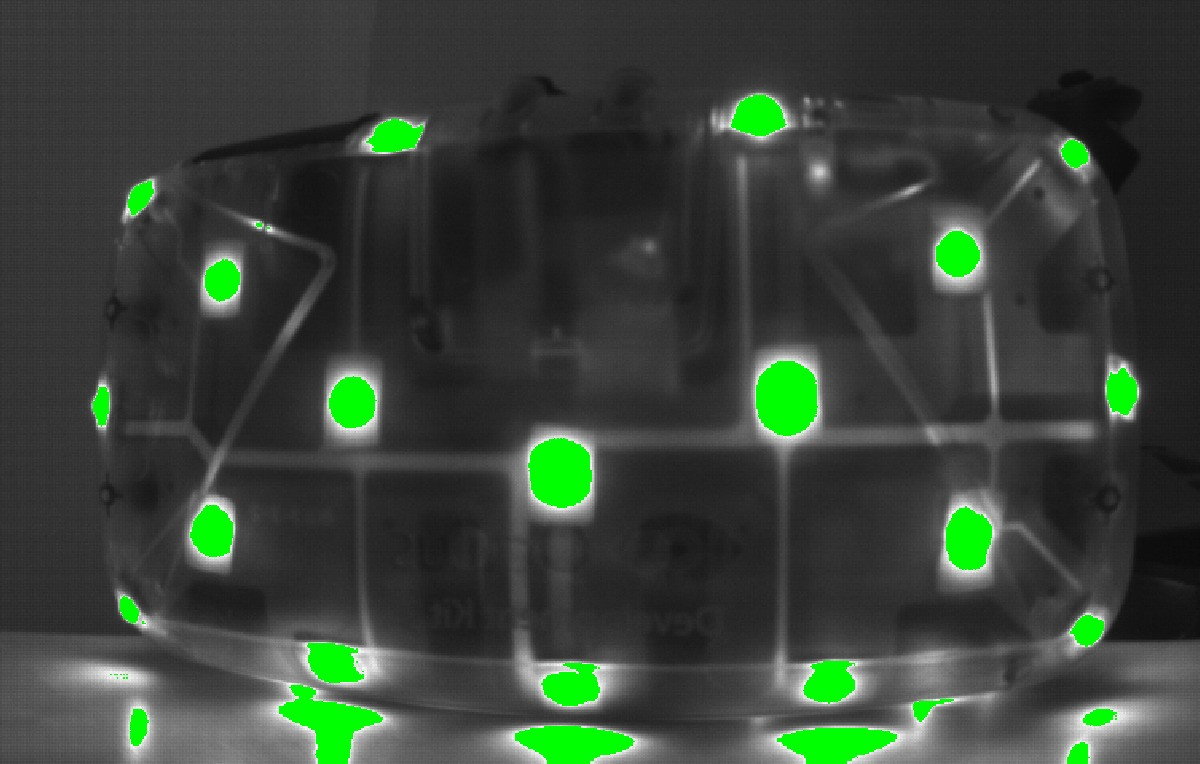
\includegraphics[width=\linewidth,height=\paperheight,keepaspectratio]{riftIR.jpg}
	\caption{Rift Sensor IR}
	%to ref fig number
	%Figure \ref{fig:block1} shows our blockDiagram.
	\label{fig:riftCam}
	\end{figure}
	\pagebreak
	\subsubsection{HTC Vive Light House Sensors}
\begin{itemize}
  \item Resolution: 752×480
  \item Refresh Rate: 16 Hz (60 FPS)
  \item Max Depth: ?
  \item Release Date: July 2014
  \item Manufacturer: Oculus Rift
  \item Cross Platform: No
  \item Skeleton Joints: Headset Position
  \item Horizontal FOV: NA
  \item Vertical FOV: NA
  \item Pixels Per Degree: NA
  \item Technique: 360 Laser / LED full room scanning 
  \item Cost: Included With Headset
\end{itemize}
\begin{figure}[H]
	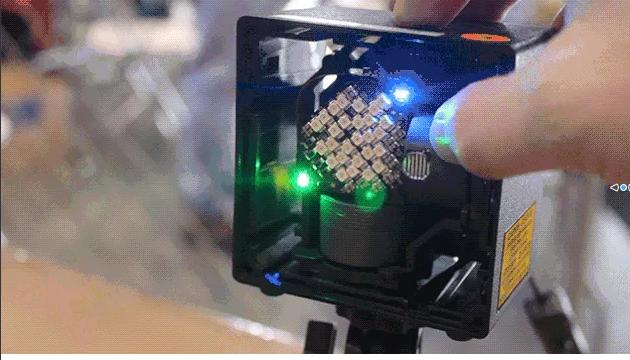
\includegraphics[width=\linewidth,height=\paperheight,keepaspectratio]{viveLight.jpg}
	\caption{HTC Lighthouse Sensor}
	%to ref fig number
	%Figure \ref{fig:block1} shows our blockDiagram.
	\label{fig:viveCam}
	\end{figure}
	\pagebreak

\subsection {Psychology research}
This Section will discuss our research and information about the psychological side of our project including a history of VR therapy, warnings, limitations, trends, other successful tests, and specifics about different phobias or disorders that we are researching. 
\subsubsection{History of VR Therapy}
The very first study on using Virtual Reality for therapy purposes was done in 1995, by Barbara Rothham and Larry Hodges.  Barbara was a researcher at Emory University with a PHD, while Larry was a computer scientist.  Together they demonstrated that virtual reality could help people overcome their fear of heights, or acrophobia.  \cite{alCarl}
%http://www.apa.org/monitor/julaug05/cure.aspx
The next year, Albert Carlin, PhD, and Hunter Hoffman, PhD, both at the University of Washington, created a study showing that Virtual Reality could help with fear of spiders, including in extreme phobia cases.  These two cases set a precedent for experimentation that continued for the next decade, with many papers and studies being published.
\par~\\
Today, VR is used for phobia and anxiety treatment in labs all over the world.  In fact, near UCF there is a major medical center focusing on this stuff, known as the Virtual Reality Medical Center.  Their website says the following about them: "The Virtual Reality Medical Center uses Virtual Reality-enhanced Cognitive Behavioral Therapy (VR-CBT) to treat clients with panic disorder, specific phobias, agoraphobia, and social phobia. Specific phobias are conditions such as fear of flying, fear of heights, claustrophobia, fear of driving, fear of thunderstorms, arachnophobia, and fear of public speaking. Virtual reality exposure therapy places you in a computer-generated world where you "experience" the various stimuli related to your phobia. You will wear a head- mounted display with small TV monitors and stereo earphones to receive both visual and auditory cues."\cite{vrPhobia}
%http://www.vrphobia.com/aboutus.htm
\par~\\
Virtual Reality therapy has grown from an idea to an industry, and we hope to take the results of that, scale them down, and bring them into user's homes.  The below section will go into the specific areas of Psychology that our project will be working with.  Meanwhile, in the specific research section for each of our 3 modules, there is more info on specific scientific studies relating to said Virtual reality therapy.
\par~\\
\pagebreak

\subsubsection{DSM Cautionary Statement}
Any cited DSM excepts following include this statement as a disclaimer. \cite{dsmCaution}
\begin{itemize}

\item The specified diagnostic criteria for each mental disorder are offered as guidelines for making diagnoses, because it has been demonstrated that the use of such criteria enhances agreement among clinicians and investigators. The proper use of these criteria requires specialized clinical training that provides both a body of knowledge and clinical skills. 

\item These diagnostic criteria and the DSM-IV Classification of mental disorders reflect a consensus of current formulations of evolving knowledge in our field. They do not encompass, however, all the conditions for which people may be treated or that may be appropriate topics for research efforts. 

\item The purpose of DSM-IV is to provide clear descriptions of diagnostic categories in order to enable clinicians and investigators to diagnose, communicate about, study, and treat people with various mental disorders. It is to be understood that inclusion here, for clinical and research purposes, of a diagnostic category such as Pathological Gambling or Pedophilia does not imply that the condition meets legal or other non-medical criteria for what constitutes mental disease, mental disorder, or mental disability. The clinical and scientific considerations involved in categorization of these conditions as mental disorders may not be wholly  relevant to legal judgments, for example, that take into account such issues as individual responsibility, disability determination, and competency.
\end{itemize}
\par~\\
To summarize, while the DSM is important and helpful, it is by no means complete.  We will be using it to get a better basic understanding but it is not perfect.  Our platform will contain a similar disclaimer.
\par
\subsubsection{DSM Criteria for Specific Phobias}
\paragraph{DSM IV}~\\
(cautionary statement) 
\begin{itemize}
\item Marked and persistent fear that is excessive or unreasonable, cued by the presence or anticipation of a specific object or situation (e.g., flying, heights, animals, receiving an
injection, seeing blood). 
\item Exposure to the phobic stimulus almost invariably provokes an immediate anxiety response, which may take the form of a situationally bound or situationally predisposed Panic Attack. 
Note: In children, the anxiety may be expressed by crying, tantrums, freezing, or clinging. 
\item  The person recognizes that the fear is excessive or unreasonable. Note: In children, this feature may be absent. 
\item The phobic situation(s) is avoided or else is endured with intense anxiety or distress. 
\item The avoidance, anxious anticipation, or distress in the feared situation(s) interferes significantly with the person's normal routine, occupational (or academic) functioning, or
social activities or relationships, or there is marked distress about having the phobia. 
\item In individuals under age 18 years, the duration is at least 6 months.
\item The anxiety, Panic Attacks, or phobic avoidance associated with the specific object or situation are not better accounted for by another mental disorder, such as Obsessive-
Compulsive Disorder (e.g., fear of dirt in someone with an obsession about contamination), Post-traumatic Stress Disorder (e.g., avoidance of stimuli associated with a severe stressor),
Separation Anxiety Disorder (e.g., avoidance of school), Social Phobia (e.g., avoidance of social situations because of fear of embarrassment), Panic Disorder with Agoraphobia, or 
Agoraphobia Without History of Panic Disorder. \cite{dsmPhobia}
\end{itemize}



\paragraph{Specific types:} 
\begin{itemize}
\item Animal Type
\item Natural Environment Type (e.g., heights, storms, water) 
\item Blood-Injection-Injury Type 
\item Situational Type (e.g., airplanes, elevators, enclosed places) 
\item Other Type (e.g., phobic avoidance of situations that may lead to choking, vomiting, or contracting an illness; in children, avoidance of loud sounds or costumed characters)
\end{itemize}
\par

\subsubsection{DSM Criteria for Anxiety Disorder}
\begin{itemize}
	\item Excessive anxiety and worry (apprehensive expectation), occurring more days than not for at least 6 months, about a number of events or activities (such as work or school performance).
	\item The individual finds it difficult to control the worry.
	\item The anxiety and worry are associated with three (or more) of the following six symptoms (with at least some symptoms having been present for more days than not for the past 6 months): (Note: Only one item is required in children.)
	\begin{itemize}
		\item Restlessness or feeling keyed up or on edge.
		\item Being easily fatigued.
		\item Difficulty concentrating or mind going blank.
		\item Irritability.
		\item Muscle tension.
		\item Sleep disturbance (difficulty falling or staying asleep, or restless, unsatisfying sleep).
	\end{itemize}
	
	\item The anxiety, worry, or physical symptoms cause clinically significant distress or impairment in social, occupational, or other important areas of functioning.
	\item The disturbance is not attributable to the physiological effects of a substance (e.g., a drug of abuse, a medication) or another medical condition (e.g., hyperthyroidism).
	\item The disturbance is not better explained by another mental disorder (e.g., anxiety or worry about having panic attacks in panic disorder, negative evaluation in social anxiety disorder social phobia, contamination or other obsessions in obsessive-compulsive disorder, separation from attachment figures in separation anxiety disorder, reminders of traumatic events in posttraumatic stress disorder, gaining weight in anorexia nervosa, physical complaints in somatic symptom disorder, perceived appearance flaws in body dysmorphic disorder, having a serious illness in illness anxiety disorder, or the content of delusional beliefs in schizophrenia or delusional disorder)\cite{dsmAnxiety}
\end{itemize}
It is important that we remain aware of this info in our project, and also attempt to inform the user as best we can.  Knowing the definitions of the most extreme version of what we are attempting to help deal with helps us to know how to deal with less extreme versions of the same issues.
\par~\\ 

\subsubsection{Exposure Therapy}
Additionally, as we will be treating with Exposure Therapy, it is important to have a definition of that.  The Society of Clinical Psychologists (a section of the American Psychology Association) includes it as one of it's empirically supported treatment options, so it is a viable option.  Following is some of the info that Society of Clinical Psychologists gives, with some info about how it relates to our project.
\par~\\ 
They define exposure therapy as, "Exposure therapy is a psychological treatment that was developed to help people confront their fears. When people
are fearful of something, they tend to avoid the feared objects, activities, or situations. Although this avoidance might help reduce feelings of fear in the short term, over the long term it can make the fear become even worse. In such situations, a psychologist might recommend a program of exposure therapy in order to help break the pattern of avoidance and fear. In this form of therapy, psychologists create a safe environment in which to "expose" individuals to the things they fear and avoid. The exposure to the feared objects, activities, or situations in a safe environment helps reduce fear and decrease avoidance. "
\par~\\ 
Additionally, they state that exposure therapy can be useful for 
\begin{itemize}
	\item Phobias
	\item Panic Disorder
	\item Social Anxiety Disorder
	\item Obsessive-Compulsive Disorder
	\item Posttraumatic Stress Disorder
	\item Generalized Anxiety Disorder 
\end{itemize}
Our project will be focusing on using exposure therapy for phobias and Social Anxiety Disorder.  
\par~\\ 
Additionally, they seperate the different ways that exposure therapy can be paced:
\begin{itemize}
	\item Graded Exposure, in which a psychologist and client create a ranked list of fears, and then slowly expose themselves to said fears, working their way up the list
	\item Flooding, in which the system is reversed, and the most feared things are dealt with first
	\item Systematic Desensitization, in which relaxing exercises and such are used to help the client associate fears with relaxation and have an easier time doing the therapy.
\end{itemize}
Our project will be using Graded Exposure, as flooding could be dangerous without a psychologist around to help, and we do not have the resources to create something that can do both relaxation and exposure therapy at the same time, which would be required for Systematic Desensitization. However, the program will come with a suggestion to try the relaxation module in between exposure therapy, potentially making said therapy easier.
\par~\\ 
Lastly, the Society defines 4 ways in which exposure therapy helps the user:
\begin{itemize}
	\item Habituation, which is the same term as forming a habit.  It means that over time, fear reactions will become lessened.
	\item Extinction, which means that Exposure Therapy can remove established connections between fears and negative results
	\item Self-efficiacy, which is the user becoming aware of their fears and becoming more able to control/manage their fears and worry
	\item Emotional Processing, which allowing the user to process their fears and emotions in a safe place, and change or create new beliefs about the things they fear, and even understand fear better.
\end{itemize}

We believe that our project will excel at the first 3 options on this list, as they can be done by a user independently.  Processing emotions is something that we can not guarantee the user will do, as we do not have the power a therapist does to communicate directly with their client.  However, our project will absolutely give users a greater power to do so, and in terms of helping users become more aware of their fears, and creating new positive connections/destroying negative ones, our project will excel. \cite{exposeTherapy}


\pagebreak

\pagebreak
\subsection{Options for Psychological Monitoring and Feedback Channels}
This is perhaps the most difficult part of the project, providing a metric for each scene to convey psychological progress. Whether it is conquering a phobia or reducing anxiety and stress levels, this topic on its own constitutes an entire project. We have looked into various methods of measuring the success of each of our scenes in order to provide users with useful feedback.

\par~\\ 
Our research has led us to multiple parameters which we can use to assess progress, most of which will be specific to a particular scene. Before we discuss those metrics, let's first take a look at how other studies have reached this goal.

\subsubsection{How have other studies provided treatment feedback?}
The majority of professional virtual reality treatment is conducted in the presence of a licensed psychologist who is able to assess the participant on the spot. In addition to this monitoring the participant is often given a questionnaire to fill out before and after treatment. Virtual Reality Medical Center (VRMC) uses this type of assessment to acquire treatment data and provide feedback to their patients. \cite{vrPhobia}

\subsubsection{Stress Analysis}
After our status presentation it came to our attention we had no plan for providing users feedback of their progress so we began research on this topic. It turns out, measuring stress is a difficult task. 
\par~\\
The most promising and simple way for a user at home to do this, we concluded, was the S Health service on Samsung smartphones. Samsung's S Health sensors can combine readings from multiple biological factors (heart rate, oxygen levels, and heartbeat consistency) to estimate a stress level. Furthermore, there is a public API available to obtain data from these sensors. This API includes an android application file that can extract recorded data from the S Health application and provides code examples for how to accomplish this. 

\begin{figure}[H]
	\centering
	\begin{minipage}{0.45\textwidth}
		\centering
		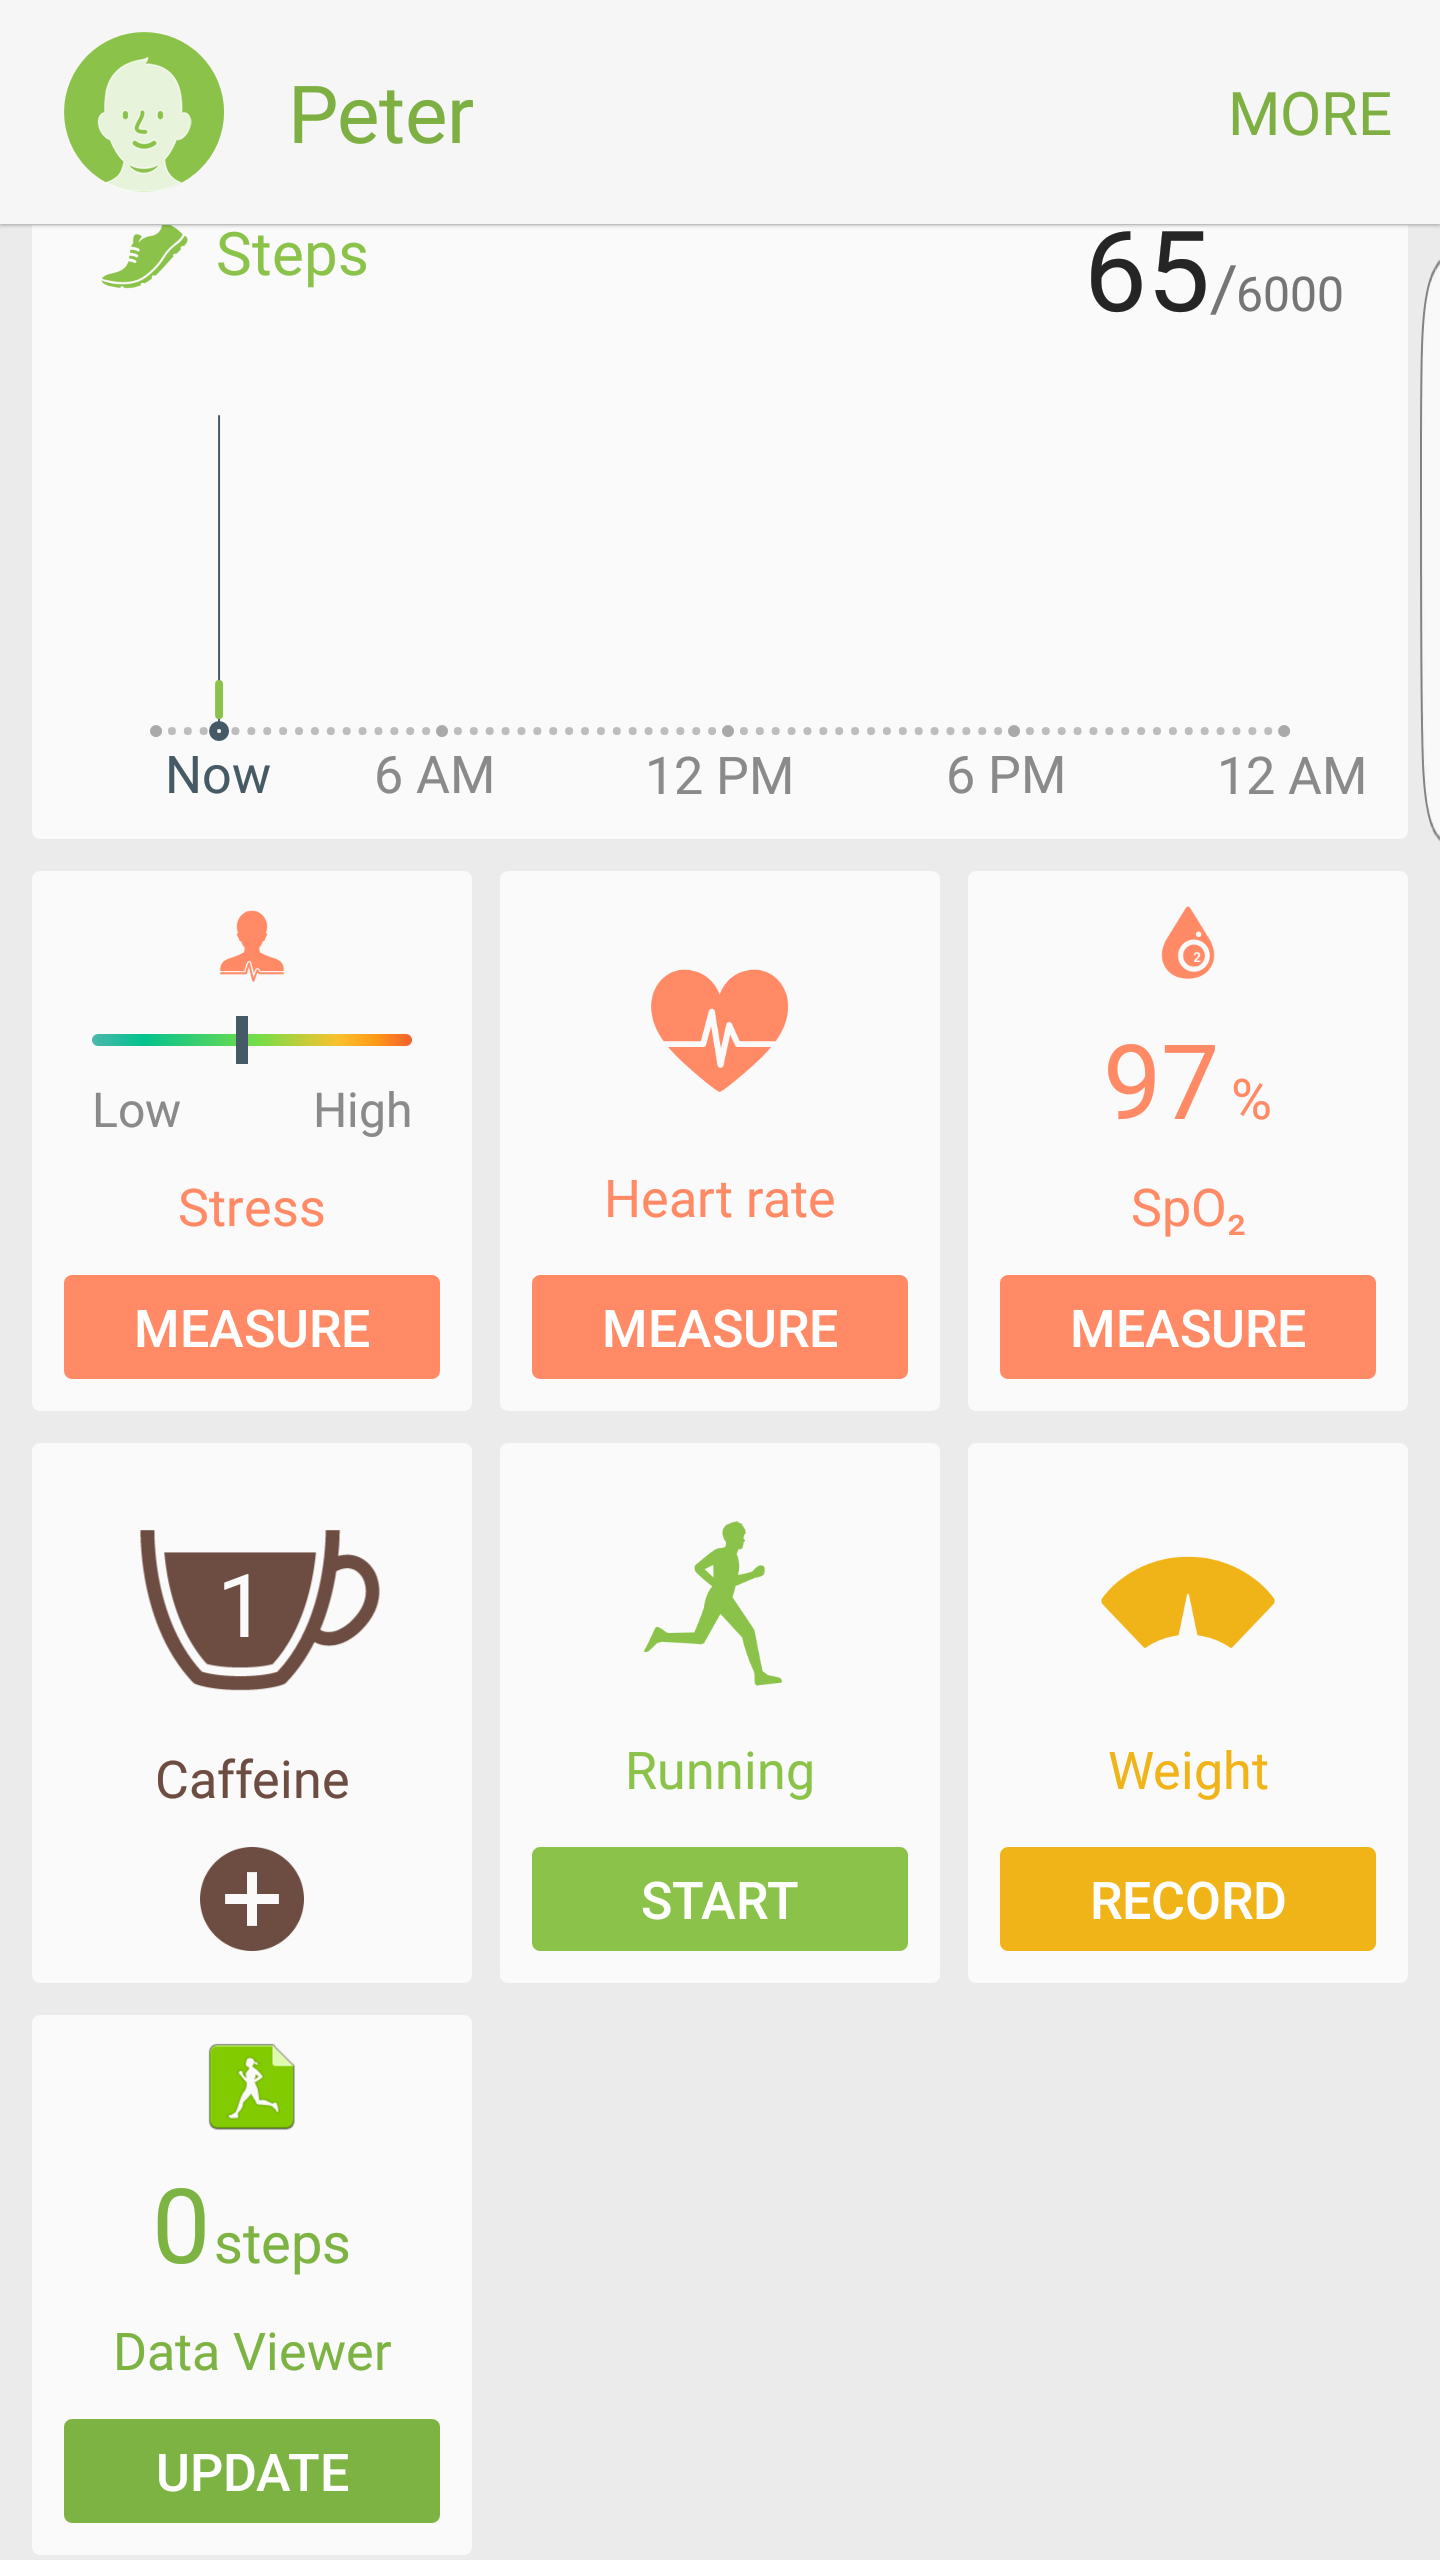
\includegraphics[scale = 0.07]{sHealthHome.png}
		\label{sHealthHome}
		\caption{S Health Home}
	\end{minipage}\hfill
	\begin{minipage}{0.45\textwidth}
		\centering
		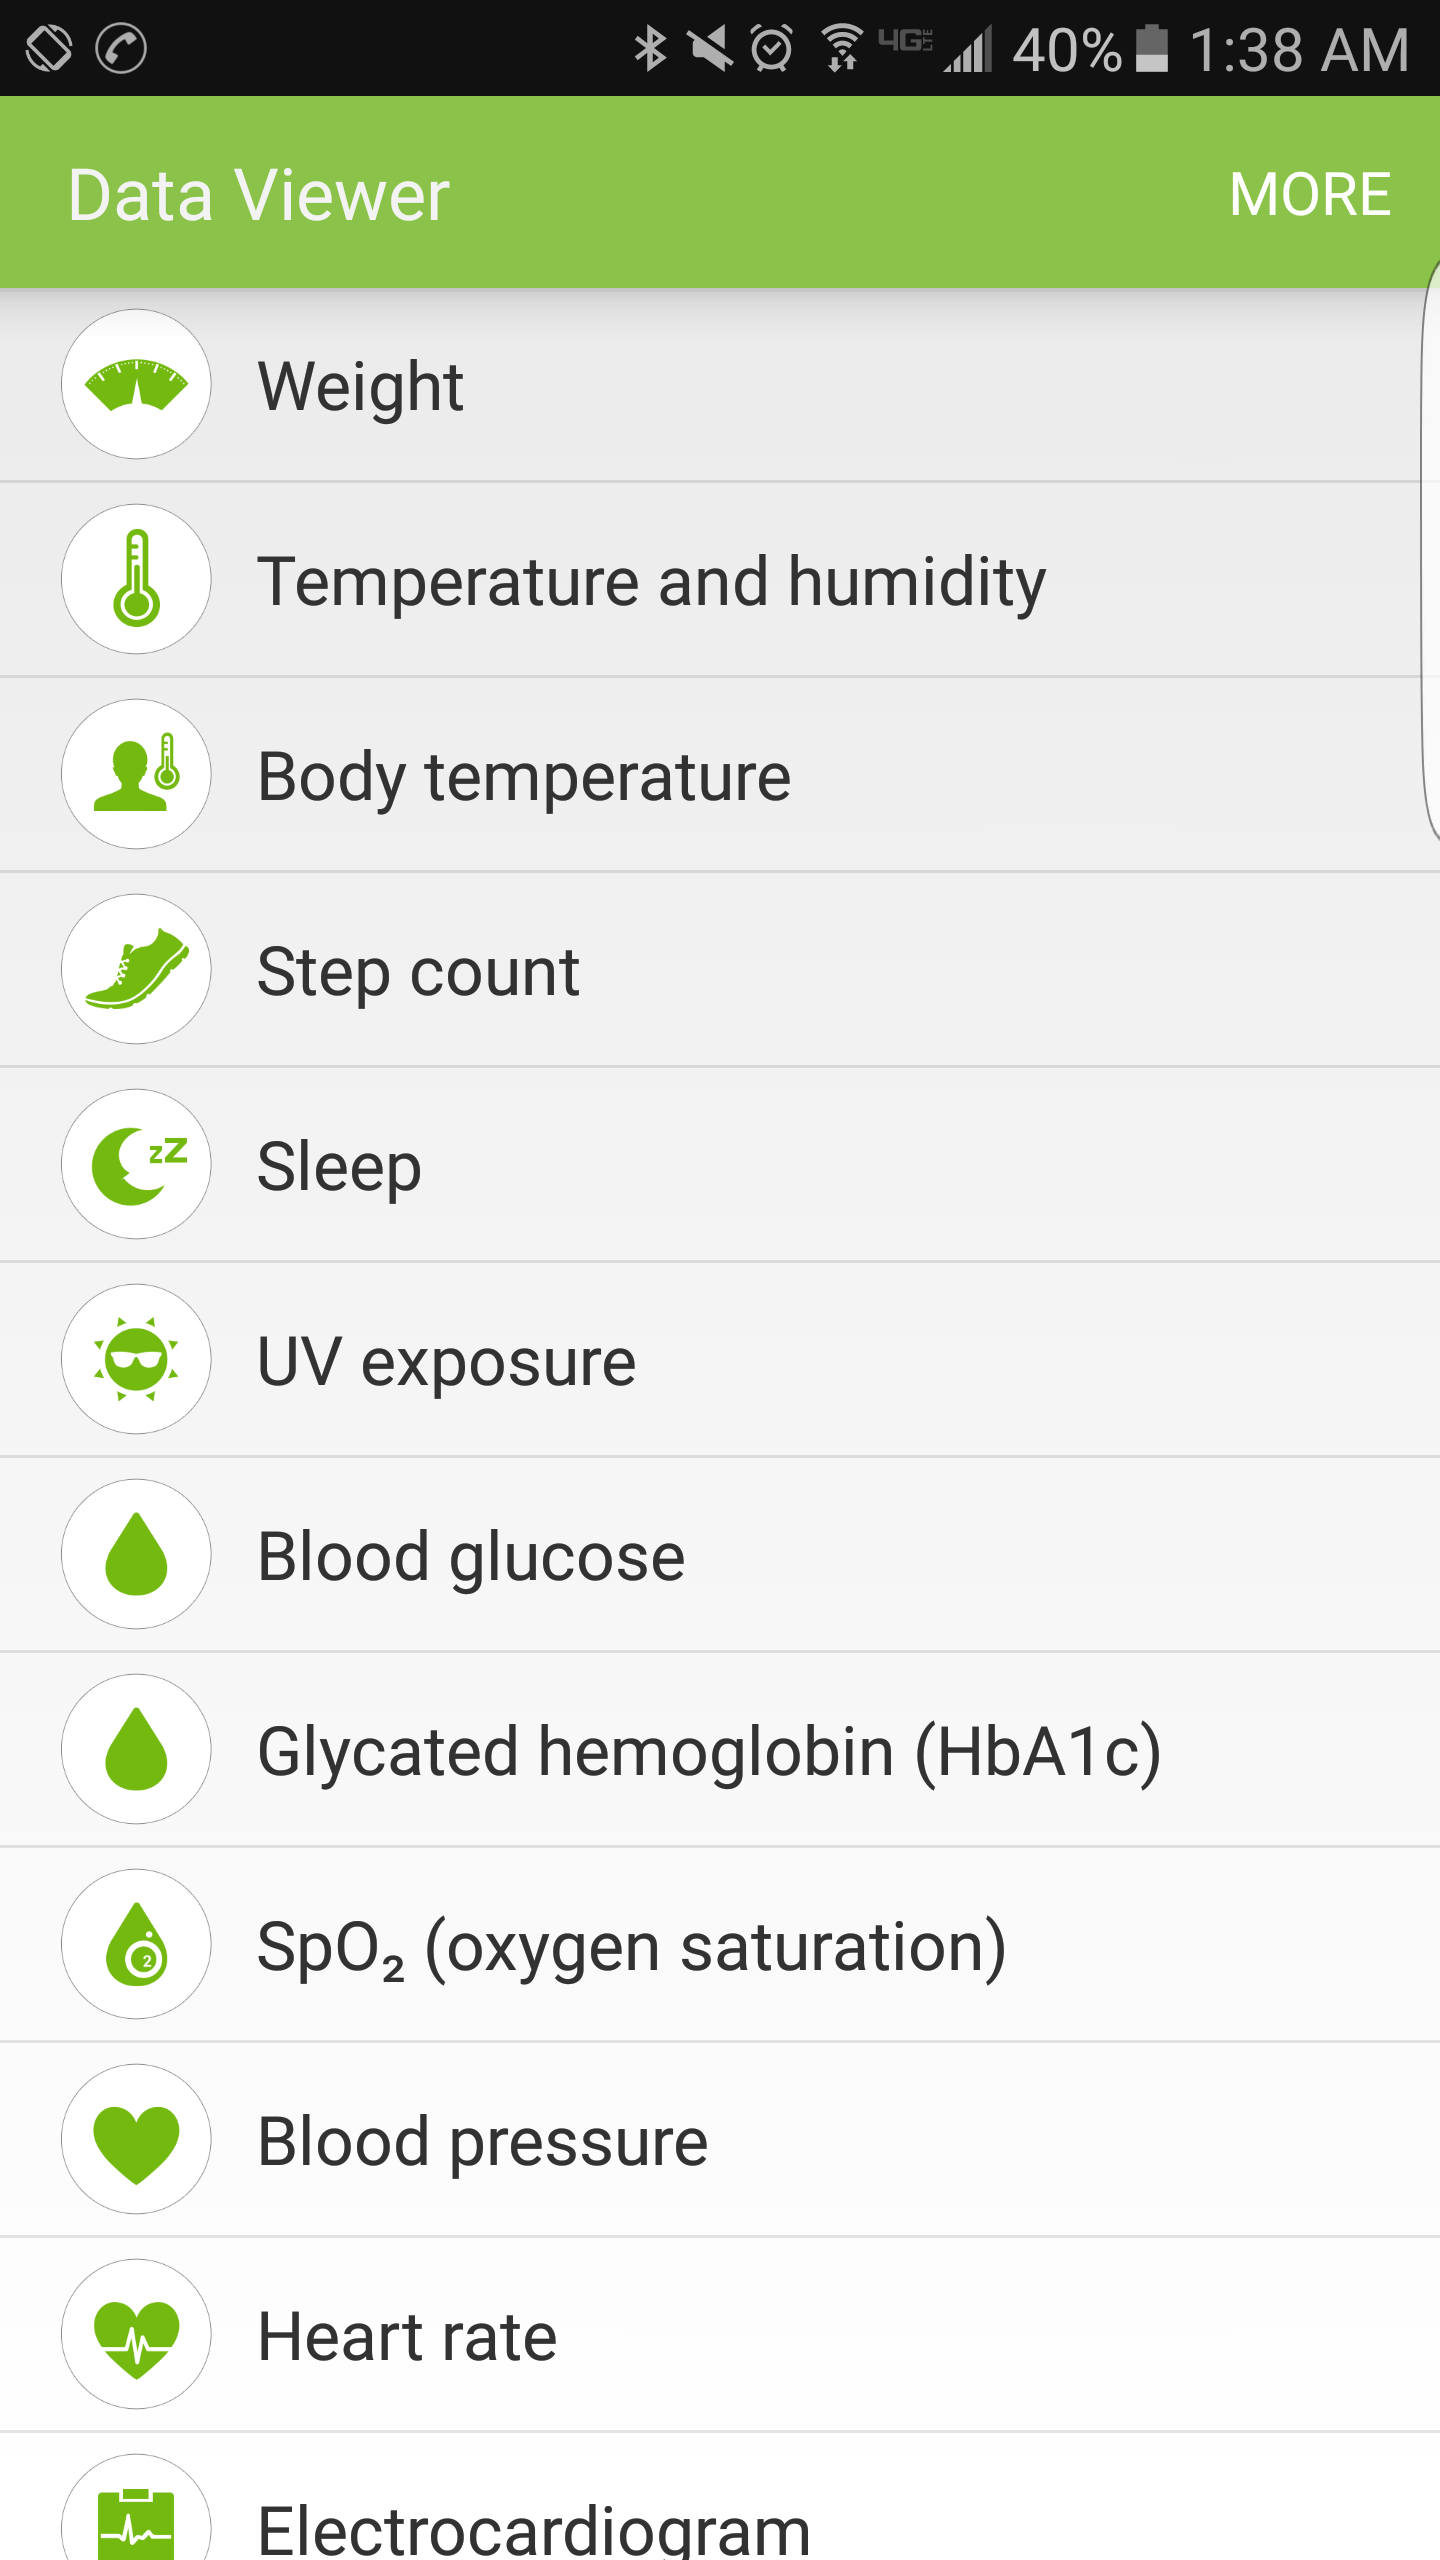
\includegraphics[scale = 0.07]{dataViewerAPK.png}
		\label{dataViewerAPK}
		\caption{S Health Data Viewer}
	\end{minipage}
\end{figure}
	
The caveat to this is Samsung has not made public their method of determining stress data nor can recorded stress values be accessed by the API. Currently, using S Health as a way to measure stress is not feasible as we would have to design stress detection from the ground up. In order for us to implement this as a metric users would need access to an eligible Samsung device, measure their stress level, and record it in our software.

\par~\\
\textbf{Update:}
We were accepted by Samsung as an S Health Partner on Thursday, Apr 28, 2016 at 12:20 AM. We will be receiving a more functional version of their S Health SDK with Partner exclusive features. We need to review the newly provided documentation in order to determine if we want to further integrate S Health data into our scene analysis and metrics.
\begin{figure}[H] %image from gmail
	\centerline {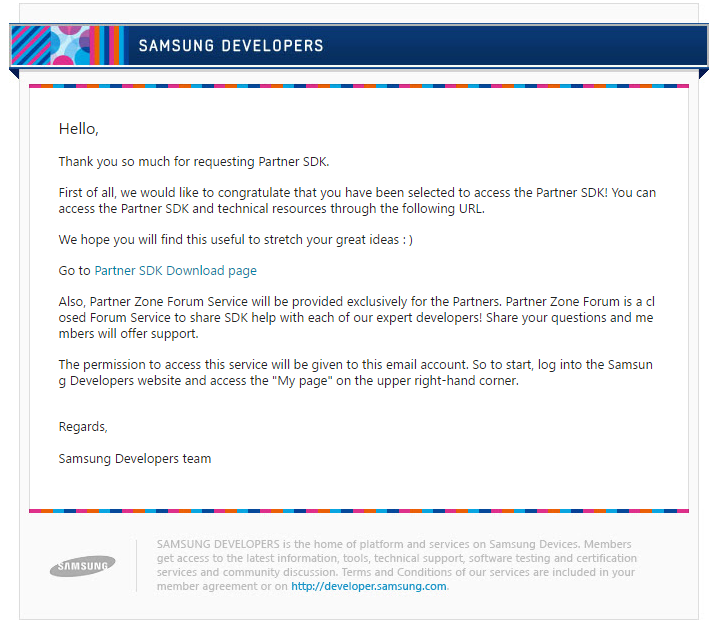
\includegraphics[scale = 0.65]{sHealthPartner.png}}
	\caption{S Health Partner Acceptance Email}
	\label{fig:sHealthPartner}
\end{figure}


\subsubsection{Stress Questionnaire}
As a stand-in for a psychologist we will be issuing a stress questionnaire. Before the user launches any scene they will be given the option of responding to questions with the goal of assessing their current level of stress. Once a scene is completed they will again be presented with this questionnaire. The before and after data will be analyzed alongside other metrics for the specific scene. Over multiple sessions this data should provide insight to whether or not the treatment is providing any benefit.

\subsubsection{Scene Progress}
Another metric we devised to provide users feedback is scene progress. This is mostly specific to our fear of heights scene. Each time the user runs the simulation the height they have reached will be recorded. Progress would be determined if the user shows reduced stress in the questionnaire along with the same or greater height.

\subsubsection{Time Spent in Stressful Simulation}
Time spent in the scene will give insight to how uncomfortable the user is. This metric can be applied to both our fear of heights scene and speech anxiety scene. If a user spends more time at a high altitude than before with relatively similar questionnaire results then it is reasonable to say the user is becoming more comfortable with their stressful situation. As for the speech anxiety scene, the user would provide an amount of time they wish to present for and over multiple sessions work to increase that time.

\subsubsection{Head Tracking}
Head tracking data from within our speech anxiety scene will function as another way to measure improvement. Time spent making eye contact with audience members compared with time spent looking elsewhere, such as the board or downward, should improve as a user becomes more comfortable with public speaking.

\subsubsection{Posture Tracking} %NEEDS WORK
Posture is a good measure of confidence. We will monitor the users posture within our speech anxiety scene to approximate their level of confidence while delivering their speech. To accomplish this we will use the Kinect sensor to follow body movement and track changes in their shoulder height throughout their presentation.


\pagebreak
\subsection{Module 1 Fear of Heights}
The fear of heights module will be built around the success of past and present research. Fear of heights, referred to as acrophobia, is a popular target for studying the impact of virtual reality on treatment. Past experiments and studies on using virtual reality for acrophobia treatment have lacked high quality graphical experiences which can detract from the immersion. Our background will feature a detailed cityscape to increase the realism which the user experiences and likely increase the effectiveness of treatment.

\subsubsection{Past Research}
In said research labs, researches have had proven that virtual reality can help with Acrophobia.  Below is a list of 4 different studies, with a brief overview of how they were run and what their results were.
\begin{itemize}
	\item In the summer of 1995, a team of researches did a case study with a single student who suffered from agoraphobia.  They 5 sessions, using VR exposure therapy , and then ran a series of tests on the student to see how it had affected them.  While their sample size was small, the case study provided evidence that VR could be used to treat Acrophobia.\cite{phobiaOne}
	%http://www.sciencedirect.com/science/article/pii/S0005789405801005
	\item In may 2002, a study was done on a larger group of 33 patients who suffered from acrophobia.  The experiment compared the effects of exposure therapy that was performed at real, high up situations, and exposure therapy that was done entirely in a virtual reality situation based on the same real, high up situation.  The experiment concluded that the VR exposure therapy was just as effective as the real exposure therapy for up to 6 months afterwards (when the experiment concluded.)\cite{phobiaTwo}
	%http://www.sciencedirect.com/science/article/pii/S0005796701000237
	\item In February 2004, researchers ran a study specifically on VR treatment of acrophobia, but comparing different types of VR treatment. They compared "cave" treatment (surrounding the subject with a full virtual environment) to simply using a VR headset.   They concluded that both were equally effective at treating acrophobia, with neither showing a significant increase in benefit over the other.  This is great news for our project, as it means a simple headset like we are using can be just as effective as a full virtual environment.\cite{phobiaThree}
	%http://www.sciencedirect.com/science/article/pii/S0005796703001396
	\item In 2015, a study was published comparing the results of VR therapy in a lab vs remote VR therapy, I. E. vr therapy that isn't conducted in the presence of a therapist but rather on the subject's own, with direction.  Six individuals were tested, 3 exposed to standard VR therapy conducted in the presence of a therapist while the other 3 had their therapy done remotely.  The study found all measures of health and growth were comparable across the two groups. This is also a huge, important element to our project as it means that VR therapy can help even without the presence of a therapist.\cite{phobiaFour}
\end{itemize}


\subsubsection{Our Implementation}
For this scene the user will start at the base of a tall building. The user be able to enter a glass elevator and select their desired floor. Once they have reached the floor they will be able to walk out onto a balcony and view the surrounding landscape. At all times there will be an option to end the simulation if the user becomes too frightened.

\subsubsection{Models and Resources}
We will need a landscape, tower, and window cleaning platform model. The Unity Asset store has several options for cityscapes and tall buildings as well as a perfectly suited window cleaning platform.
\par~\\ 
As far as cityscapes go we are considering four options:
\begin{figure}[H] %https://www.assetstore.unity3d.com/en/#!/content/38412
	\centerline {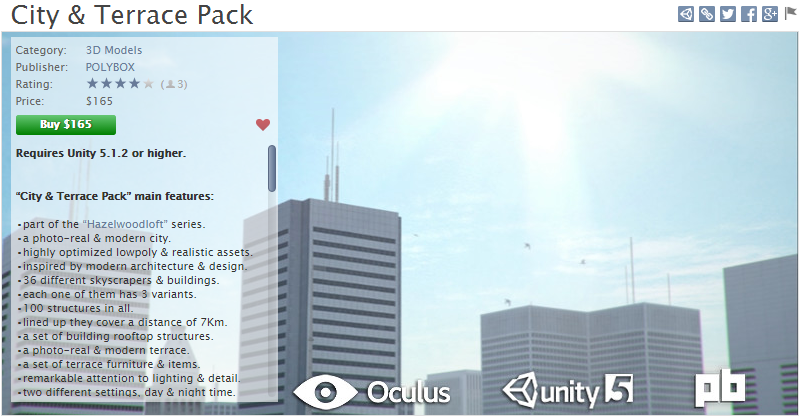
\includegraphics[scale = 0.50]{cityAndTerracePack.png}}
	\caption{City and Terrace Pack Unity Asset Store Entry}
	\label{fig:cityAndTerracePack}
\end{figure}
\begin{figure}[H] %https://www.assetstore.unity3d.com/en/#!/content/36182
	\centerline {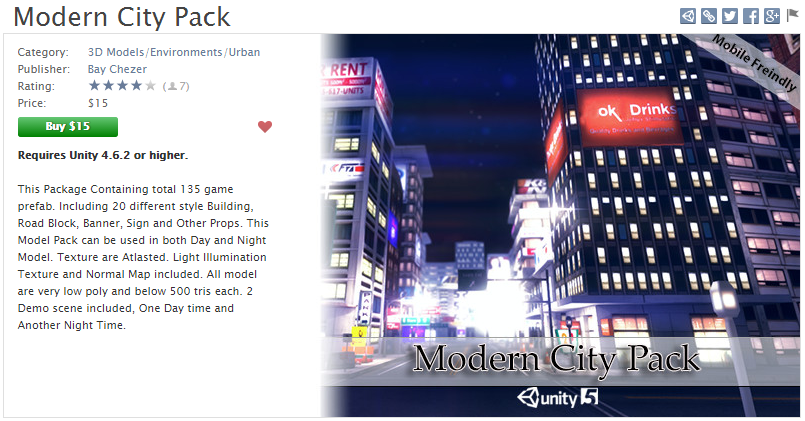
\includegraphics[scale = 0.50]{modernCityPack.png}}
	\caption{Modern City Pack Unity Asset Store Entry}
	\label{fig:modernCityPack}
\end{figure}
\begin{figure}[H] %https://www.assetstore.unity3d.com/en/#!/content/57733
	\centerline {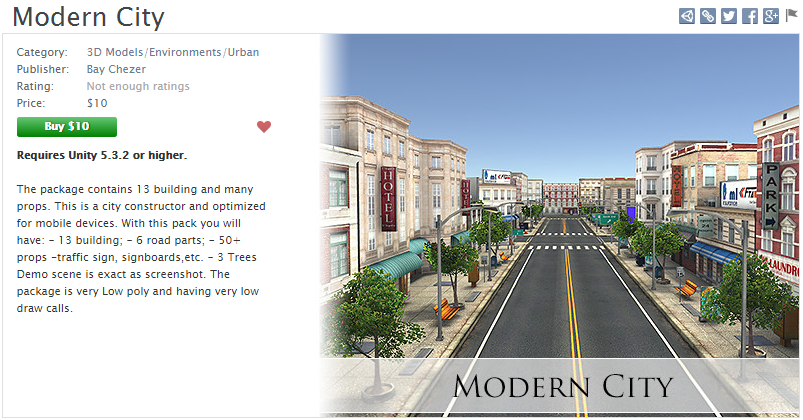
\includegraphics[scale = 0.50]{modernCity.png}}
	\caption{Modern City Unity Asset Store Entry}
	\label{fig:modernCity}
\end{figure}
\begin{figure}[H] %https://www.assetstore.unity3d.com/en/#!/content/60832
	\centerline {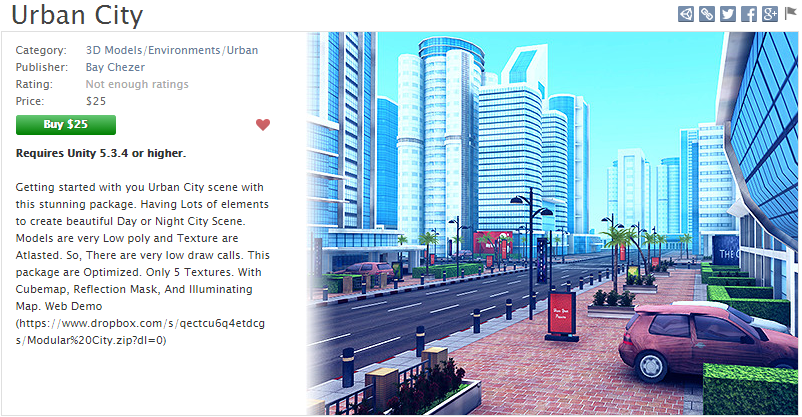
\includegraphics[scale = 0.50]{urbanCity.png}}
	\caption{Urban City Unity Asset Store Entry}
	\label{fig:urbanCity}
\end{figure}
Currently we plan on implementing the Urban City pack as our environment due to it's high quality and tall structures. As a stretch goal we may implement the ability for the user to switch between some of these landscapes to provide more variety to the environment.
\par~\\
For our elevator we will be using a window cleaning platform:
\begin{figure}[H] %https://www.assetstore.unity3d.com/en/#!/content/59736
	\centerline {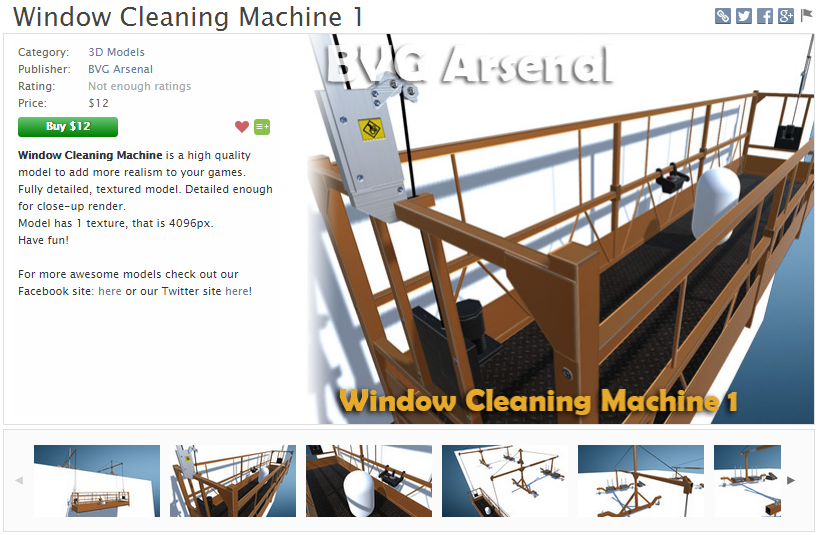
\includegraphics[scale = 0.50]{elevator.png}}
	\caption{Window Cleaning Machine Unity Asset Store Entry}
	\label{fig:elevator}
\end{figure}
The user will be able to interact with controls on the platform via Leap Motion to scale the building up and down.
\subsubsection{Interaction and User Inputs}
Interaction with this scene will be use simple look and click mechanics. Looking will be controlled by head tracking on the Oculus Rift and clicking will be controlled with Leap Motion. While on the elevator platform the user will have access to a control panel to set the height of the platform between ground floor and the top of the building. The user will also be able to abort the scene at any time should they become too frightened. 

\subsubsection{Configuration from Qt Launcher}
Configurations in module 1 are mostly a stretch goal if we have time after completing our other scenes. Since our configuration here would be additional environments and buildings, the assets for this can become expensive quickly.

\subsubsection{User Progress Feedback}
Users may optionally respond to a questionnaire before and after the scene. The use of the Samsung S Health app will be suggested but is also optional. For this the user would run the app on their smartphone and fill in our software with the feedback given to them from the S Health stress sensor. In addition to this the scene will track how high up the user went and how much time was spent at each level. All of these metrics will be combined and analyzed over multiple sessions to provide the user feedback on their efforts.%NEEDS WORK

\pagebreak
\begin{figure}[H] %https://www.assetstore.unity3d.com/en/#!/content/59736
	\centerline {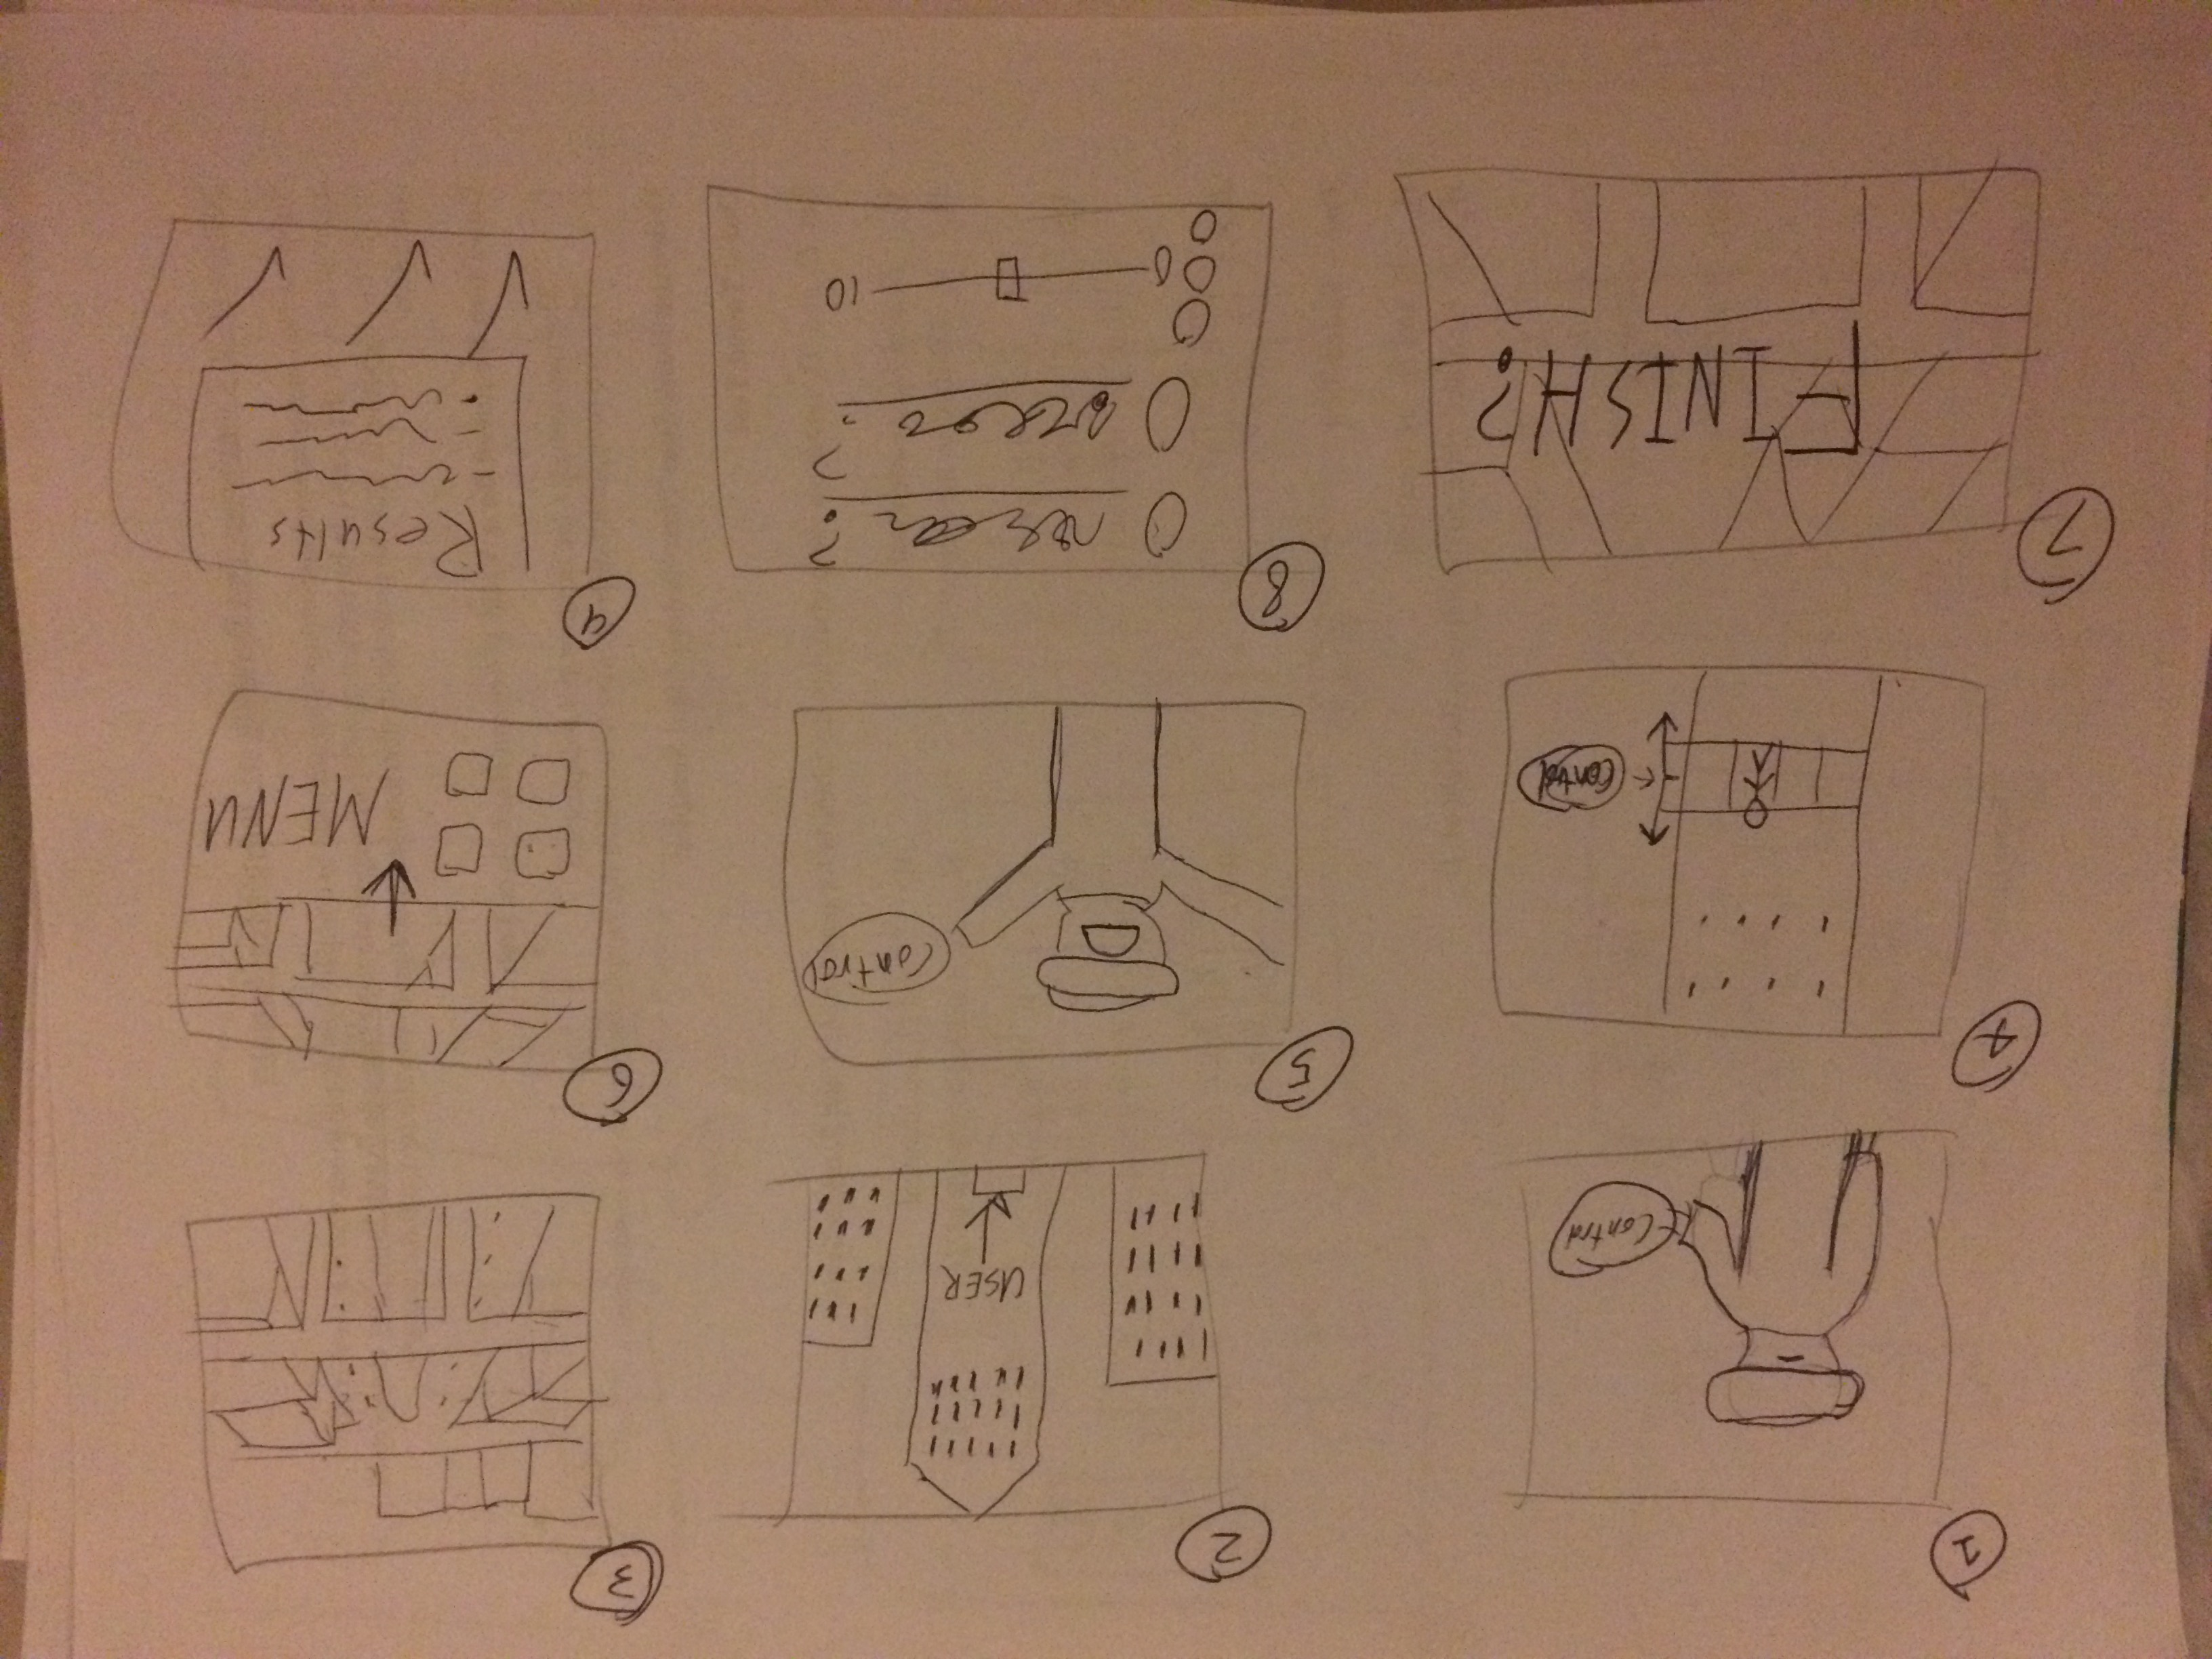
\includegraphics[scale = 0.13, angle = 180]{sbHeight.jpg}}
	\caption{Storyboard for Acrophobia Module}
	\label{fig:elevator}
\end{figure}
\begin{enumerate}
	\item The user turns on the vr, and starts the acrophobia module
	\item The user will be placed near a platform at the bottom of a very tall building
	\item The platform can move up and down on the building
	\item The user controls how the platform moves up and down with their controller
	\item If the user in anyway becomes panicked, they can hit a panic button
	\item This will remove them from the experience entirely, no questions asked.
	\item When the user either decides they are finished, or reaches the top
	\item They are asked to fill out a stress and emotion questionnaire
	\item They are then shown a results screen, that is based on data acquired from sensors, from how high they went/time it took, and their questionnaires.
\end{enumerate}
\pagebreak
\subsection{Module 2 Speech Anxiety Simulator}
Speech Anxiety is the next issue we wish to treat with virtual reality therapy. As another popular target of VR therapy research, speech anxiety has several successful examples.

\subsubsection{Past Research}
Just like for the Acrophobia section, here are some studies that have been done on the effectiveness of treating social anxiety with VR.
\begin{itemize}
	\item In July 2004, a study was done on 8 students, with a 6 person control group, to test the effectiveness of VR treatment for public speaking anxiety.  The tests were simple and conclusive; the VR treatment was, in fact, very effective at treating people according to the self reports, surveys, and heart rate measurements.\cite{anxOne}
	%http://online.liebertpub.com/doi/abs/10.1089/109493102321018187
	\item In 2013, a study was done similarly to the acrophobia study above that compared in vivo ("real") exposure therapy with Virtual Reality exposure therapy for social anxiety disorder.  This included 8 sessions of therapy, and a 12 month follow up period.  The researches concluded that VR exposure therapy was just as effective as in vivo exposure therapy.  Once again, this is fantastic for our platform as it means we VR therapy can work for social anxiety disorder..\cite{anxTwo}
	%http://psycnet.apa.org/journals/ccp/81/5/751/
	\item In 2014, a study was conducted on the use of Video Self Modeling to treat social anxiety disorder.  VSM is the use of watching oneself complete a task successfully on video in order to help oneself become able to do said task.  The study tested 101 students and found that in general, for the purpose of social anxiety disorder, VSM was not an effective treatment.  Therefore for our project we will be avoiding this specific type of treatment.\cite{anxThree}
	%http://cornerstone.lib.mnsu.edu/etds/30/
\end{itemize}

\subsubsection{Our Implementation}
In our implementation the user will be able to configure the environment in which they practice public speaking to better suit their needs and deliver a more personal experience. We will begin with a classroom environment with chair spots which the user can place different students into and configure their actions such as sleeping, focused, or texting. As a stretch goal for this module we will implement more varying environments like a conference room and a stage.

Presentation will begin with the user sitting down. Momentarily they will be called upon to present and must stand and walk to the front of the room. If they have a power point preloaded through Qt they will walk to the front desk and plug it into the equipment which will display it onto the screen behind them as in an actual classroom. Following this the user will deliver their speech to the configured audience. Once finished, the user will sit back in their seat and the scene will end.

\subsubsection{Models and Resources}
For the speech anxiety module we need a room for the user to practice public speaking in, relevant objects to go in it, and human models to listen to the speaker. The majority of models used for this scene will be designed in Google SketchUp while the human models will be created in MakeHuman. 

\par~\\
We will create a model of UCF's Harrison Engineering Corp. building room 108 for our first configurable room and if there is enough time we will design more options for the practice environment such as a lecture hall or conference room. Our classroom model will include the presentation equipment (projector, drop down screen, etc.) so that the user may practice the speech as close as possible to how it would actually be delivered. The room will be designed in Google SketchUp and objects such as chairs and presentation equipment will be sourced from the Google SketchUp 3D Warehouse.

\par~\\
For audience members we originally planned to use human models from the Unity Asset store but there were few models that fit our purpose and most were very expensive relative to how we will be using them. Instead of sourcing our human models from the asset store we will be designing them with a free tool called MakeHuman. 
\begin{figure}[H] %screenshot taken by Peter Lomason
	\centerline {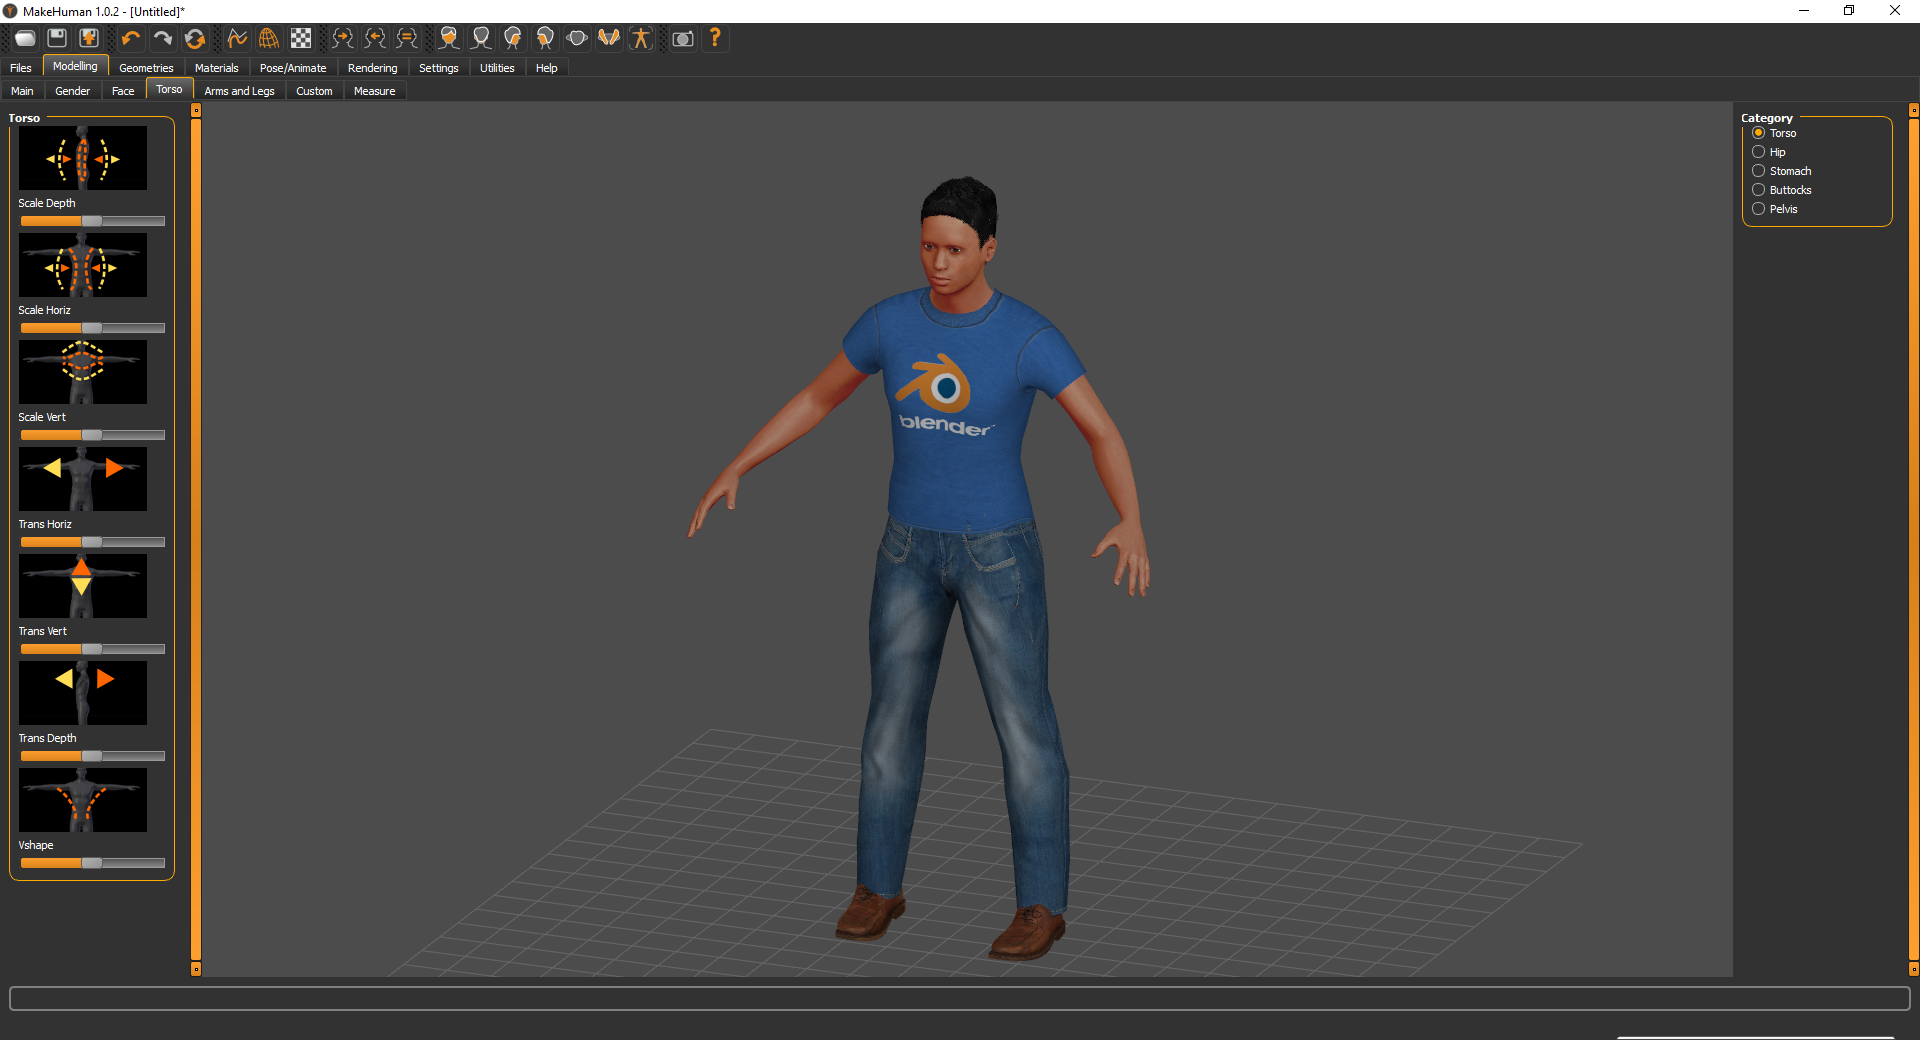
\includegraphics[scale = 0.28]{makeHuman.png}}
	\caption{MakeHuman Model Editor}
	\label{fig:makeHuman}
\end{figure}
\par~\\
This tool allows us to design a human model to our liking with free features, clothes, and more found on the community website: http://www.makehumancommunity.org/.
\par~\\
\begin{figure}[H] %screenshot taken by Peter Lomason
	\centerline {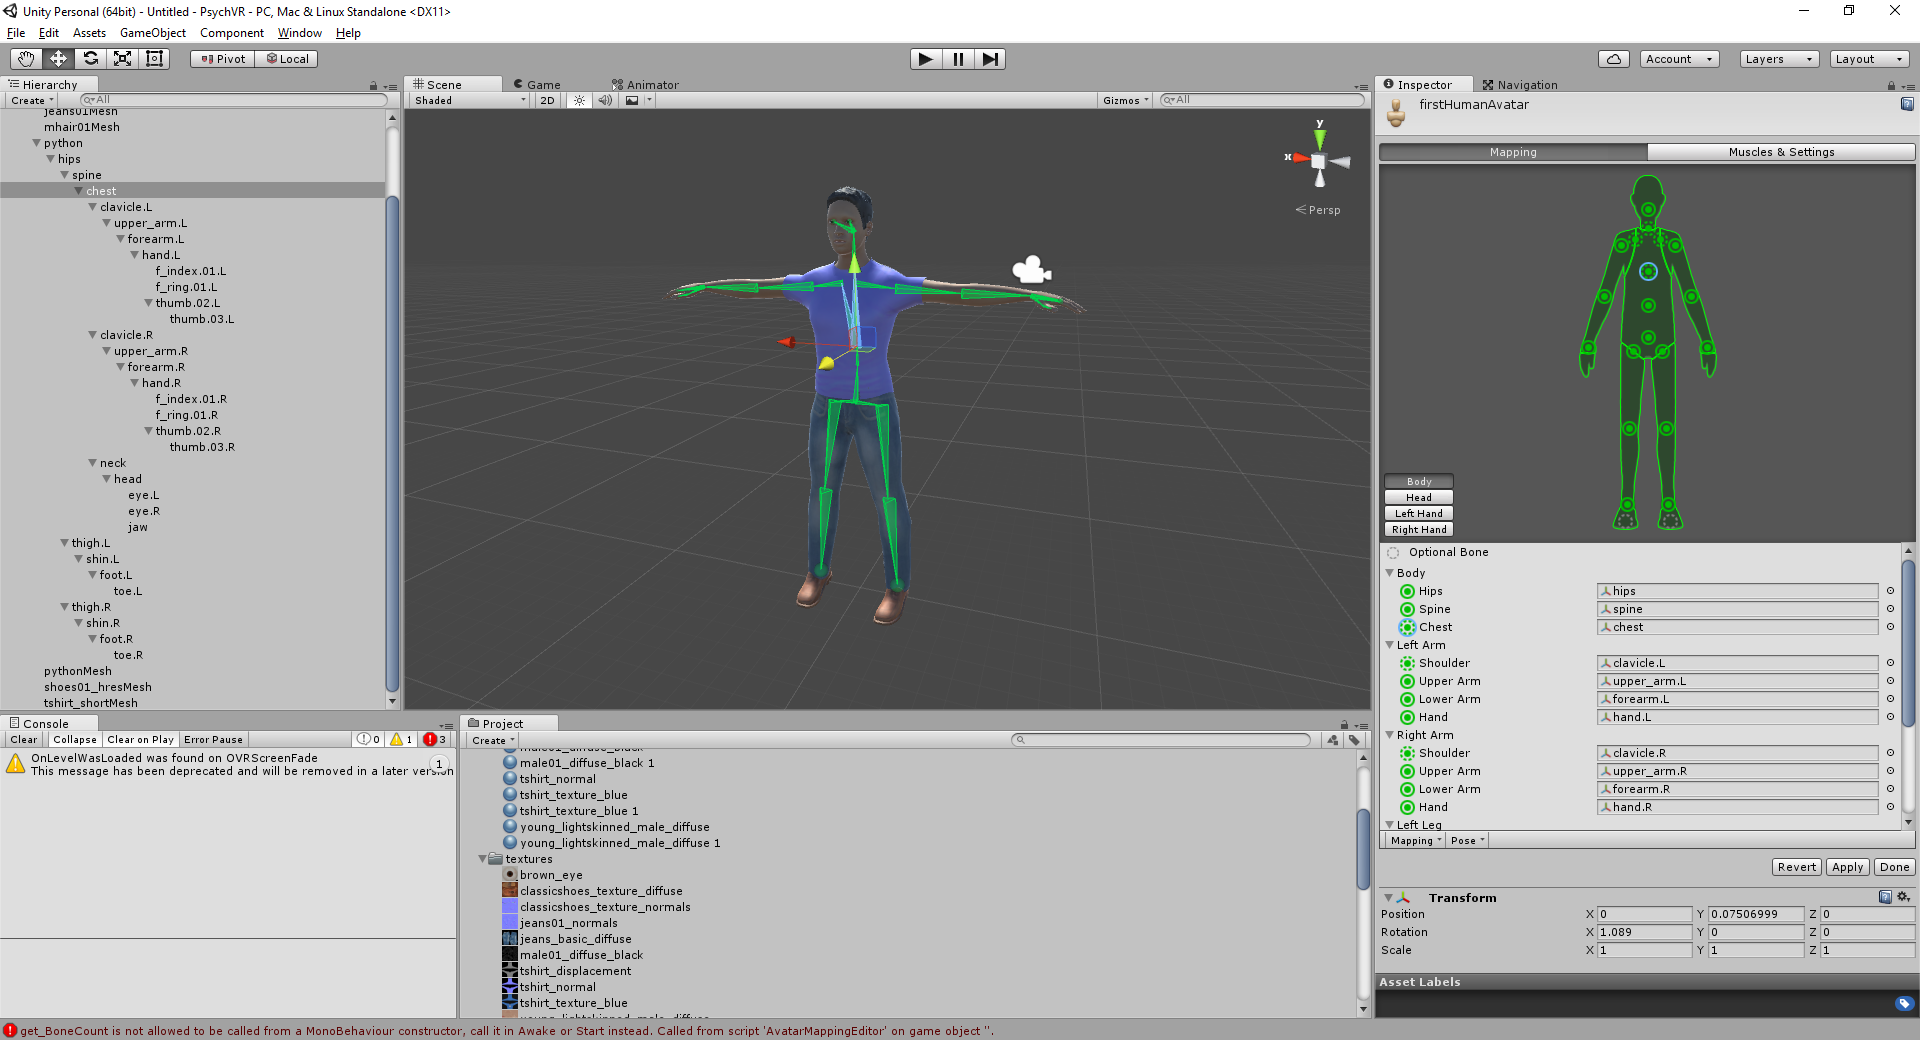
\includegraphics[scale = 0.28]{unityMecanim.png}}
	\caption{Bone Model in Unity Mecanim}
	\label{fig:unityMecanim}
\end{figure}
Models created in MakeHuman are fully rigged and can be exported as fbx files. This format is compatible with Unity's Mecanim which will be used to animate our models so they can perform various actions. These actions can be set according to how the user has configured the environment in our Qt launcher.

\subsubsection{Interaction and User Inputs}
The user begins the scene by moving from their desk to the front of the room. From here they may prepare any presentation materials they configured through Qt such as a Powerpoint presentation. Movement will be controlled via an input device which we will determine as we progress in development, we plan to control object interactions with LeapMotion. 

\subsubsection{Configuration from Qt Launcher}
This scene will be our most configurable. Qt will allow the user to specify which chairs have a model in them and what behavior that model will perform. A user will also be able to include a Powerpoint during configuration so they may have a presentation aid during their practice. As a stretch goal we hope to include more than just a classroom setting and allow users to pick from a few environments.

\subsubsection{User Progress Feedback}
Users may optionally respond to a questionnaire before and after the scene. The use of the Samsung S Health app will be suggested but is also optional. For this the user would run the app on their smartphone and fill in our software with the feedback given to them from the S Health stress sensor. In addition to these optional metrics, throughout the scene the users posture, head, and where they are looking (ex: eye contact) will be tracked in order to provide feedback about their performance during the scene. All of these metrics will be combined and analyzed over multiple sessions to provide the user feedback on their efforts.

\begin{figure}[H] %https://www.assetstore.unity3d.com/en/#!/content/59736
	\centerline {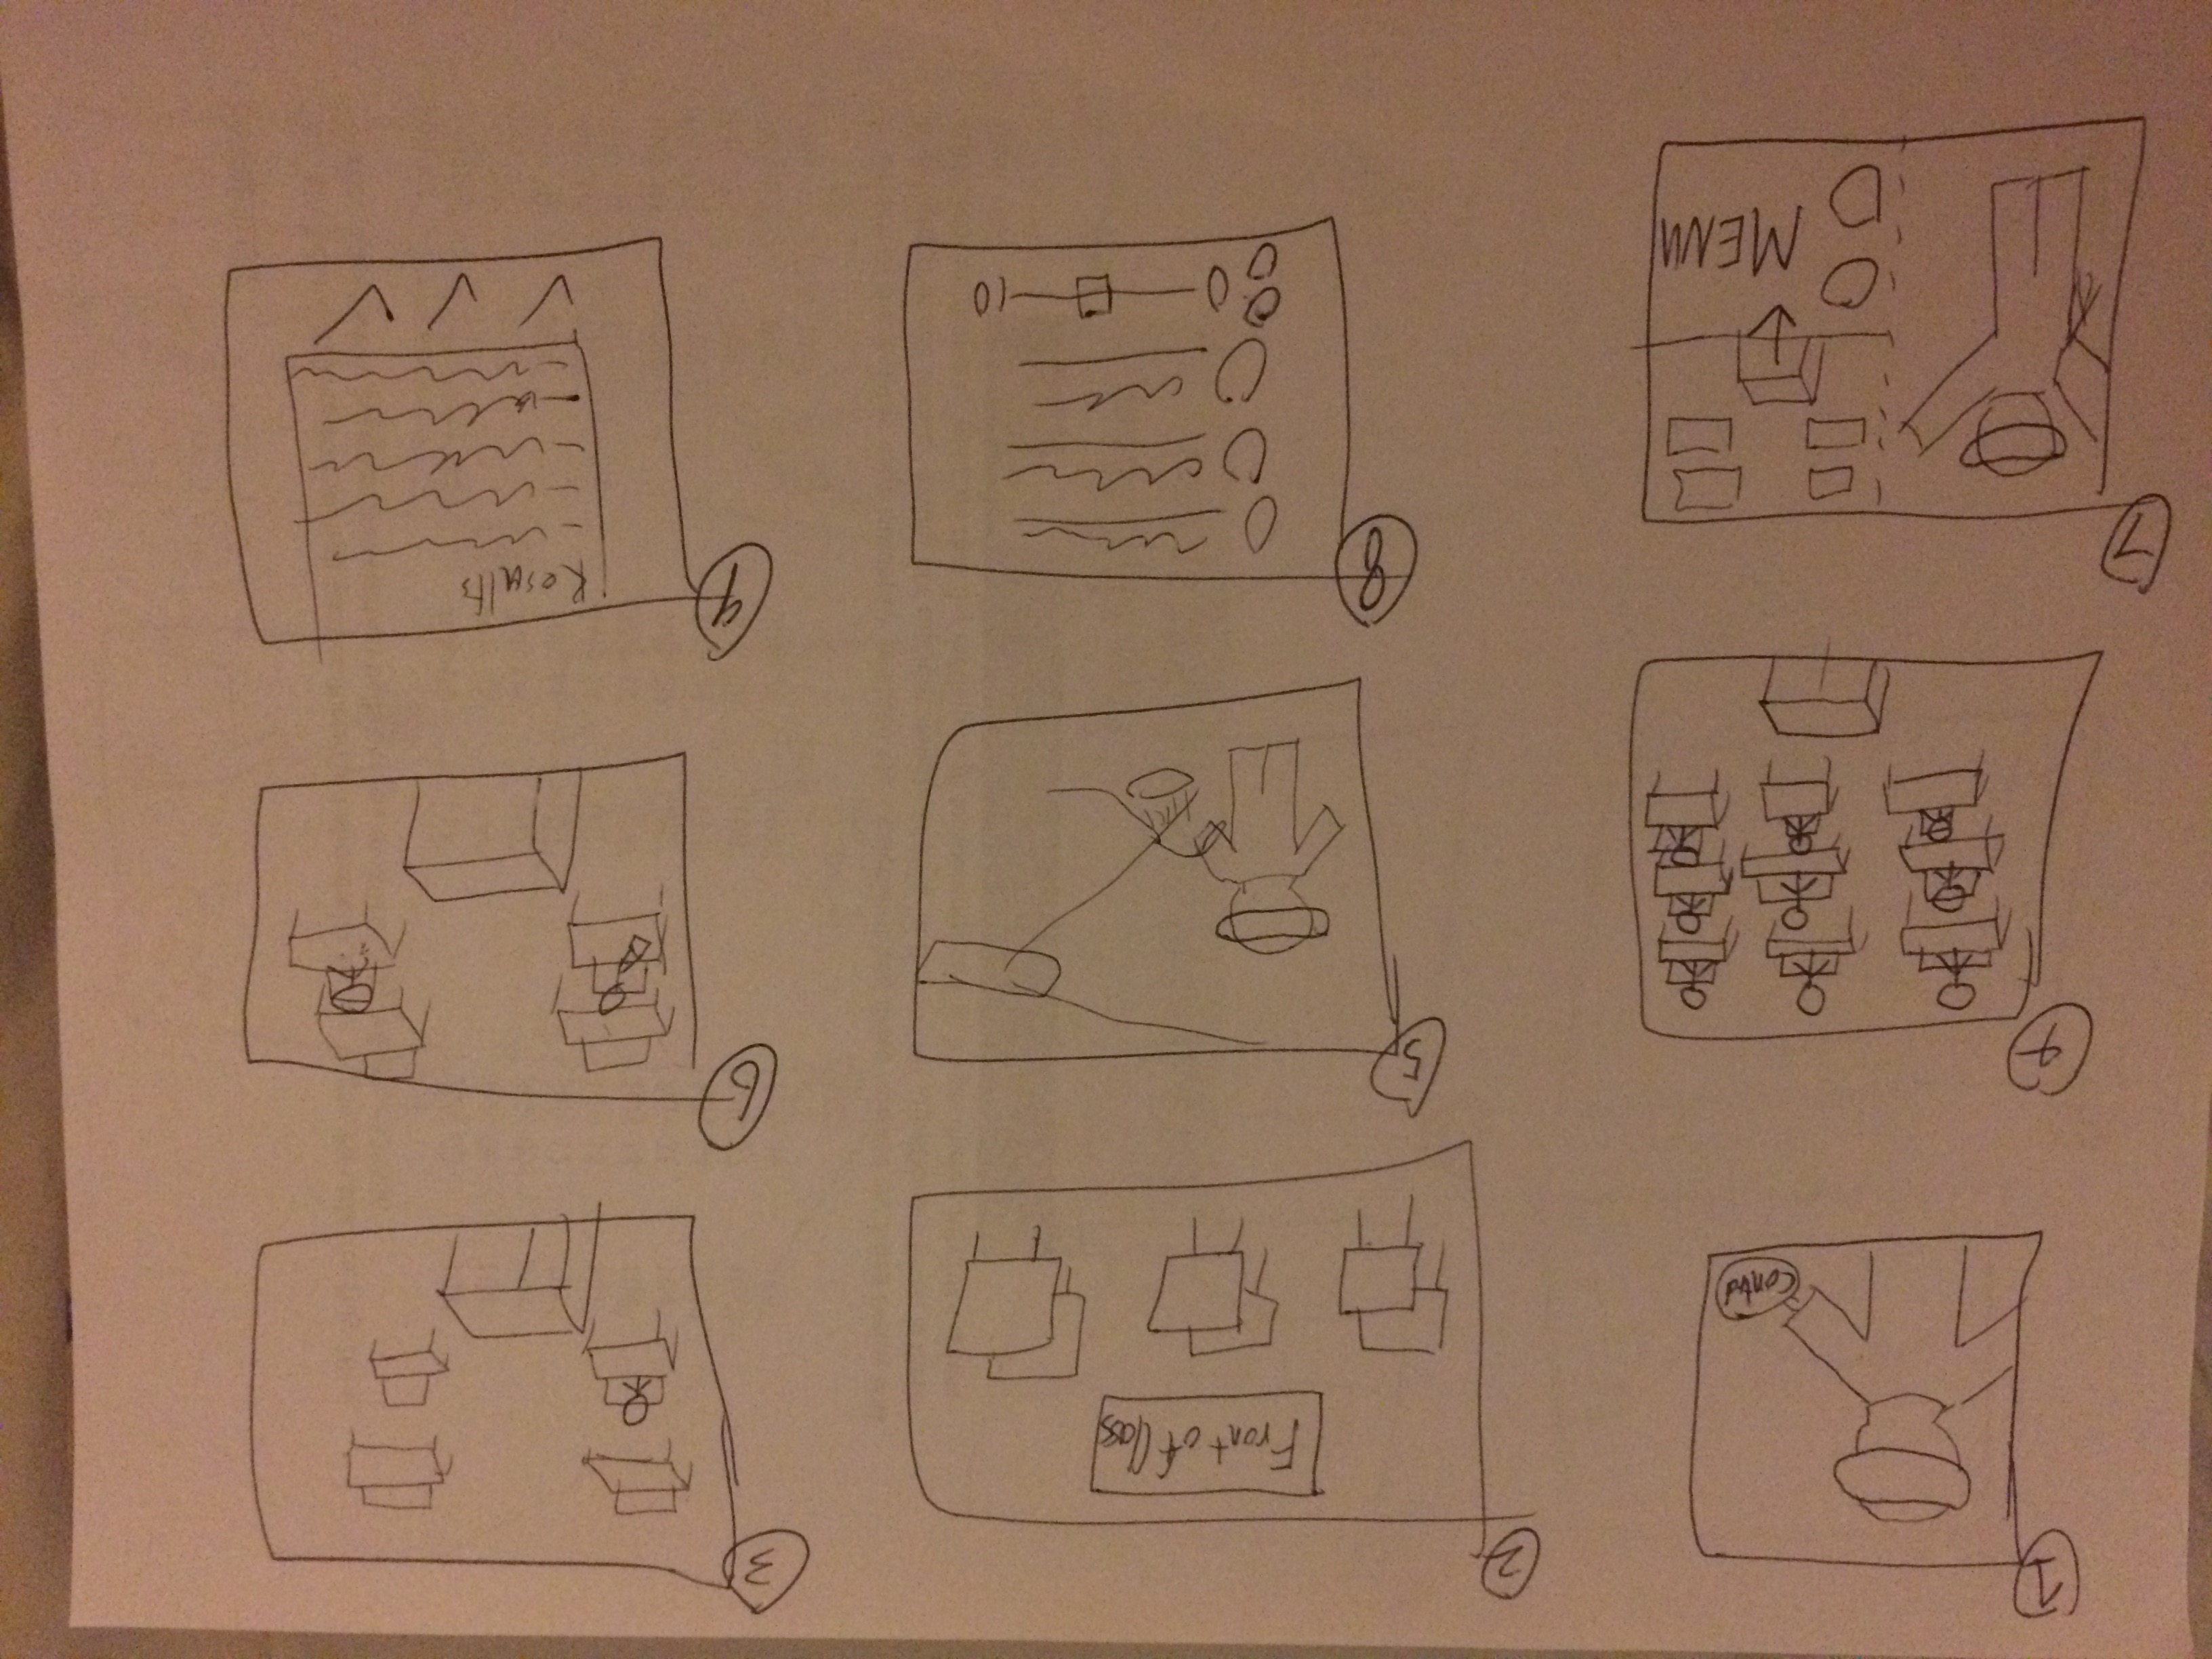
\includegraphics[scale = 0.12, angle = 180]{sbPresent.jpg}}
	\caption{Storyboard for Social Anxiety Module}
	\label{fig:elevator}
\end{figure}
\begin{enumerate}
	\item The user turns on the vr, and starts the acrophobia module
	\item The user will be in a classroom, and be asked to give a presentation.
	\item The user will use the control to move to the front of the class
	\item The number of people, attitudes, and size of the classroom will be customizable through the QT app
	\item Through measurements like the Samsung sensor, Kinect, and leap motion the user's actions while presenting will be measuring
	\item The user will do their presentation in the virtual space
	\item If the user in anyway becomes panicked, they can hit a panic button, and remove them from the experience
	\item They are asked to fill out a stress and emotion questionnaire
	\item They are then shown a results screen, that is based on data acquired from sensors and their questionnaires.
\end{enumerate}
\pagebreak
\subsection{Module 3 Calm Environment} % SO HYPED!!!
This module will feature a calming environment that will help patients with stress or anxiety relax in a calming peaceful environment. This environment will have random terrain which will have chunks that are procedurally generated while the user moves throughout the scene.  The art style/ graphic design for this project is inspired by indie games like Minecraft, Myst, or Proteus \textbf{(See Figure \ref{fig:proteus})}, except without puzzles or enemies. It will feature simple generated terrains that form a  peaceful landscape which the user can move throughout with various plants or natural features that decorate the scene.  Some configuration options for this scene include different color patterns or selecting what models are loaded or how the scene looks in general. 

\begin{figure}[H]
	\centerline{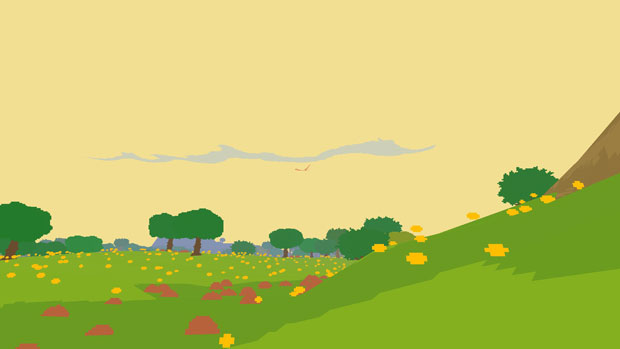
\includegraphics[scale= 0.4]{proteus.jpg}}
	\caption{Proteus Screenshot}
	%Figure \ref{fig:gpgpuImg} shows our blockDiagram.
	\label{fig:proteus}
\end{figure}

\subsubsection{Past Research}
As before, here is some past research into the field of anxiety and VR.
\begin{itemize}
	\item A study done in 2010 concluded that creating an enviroment to help subjects with GAD (Generalized Anxiety Disorder) was helpful in dealing with their GAD.  However, it also discovered that the project could be made even more effective if biofeedback from the user is incorporated into the enviroment.  This is something we will have to consider, although it may be too complex and too resource heavy for our project. \cite{calmOne}
	%https://www.researchgate.net/profile/Claudia_Repetto2/publication/44668615_Virtual_reality_in_the_treatment_of_generalized_anxiety_disorders/links/0922b4f8e9de327968000000.pdf
	\item Another expiriment tried to teach cancer patients both relaxation and Tai Chi methods to see if these things were easier to do through VR, and what effects the VR would have on them.  It found that giving the user an area that they were in charge of could possibly help people who felt like they had no control over their lives. This is a positive thing we will try to recreate with our project.
	%https://www.researchgate.net/profile/David_Becker10/publication/2659560_Using_A_Virtual_Environment_to_Teach_Cancer_Patients_T'ai_Chi_Relaxation_and_Self-Imagery/links/53ce75e80cf279d93530ac34.pdf
\end{itemize}
\pagebreak

\begin{figure}[H] %https://www.assetstore.unity3d.com/en/#!/content/59736
	\centerline {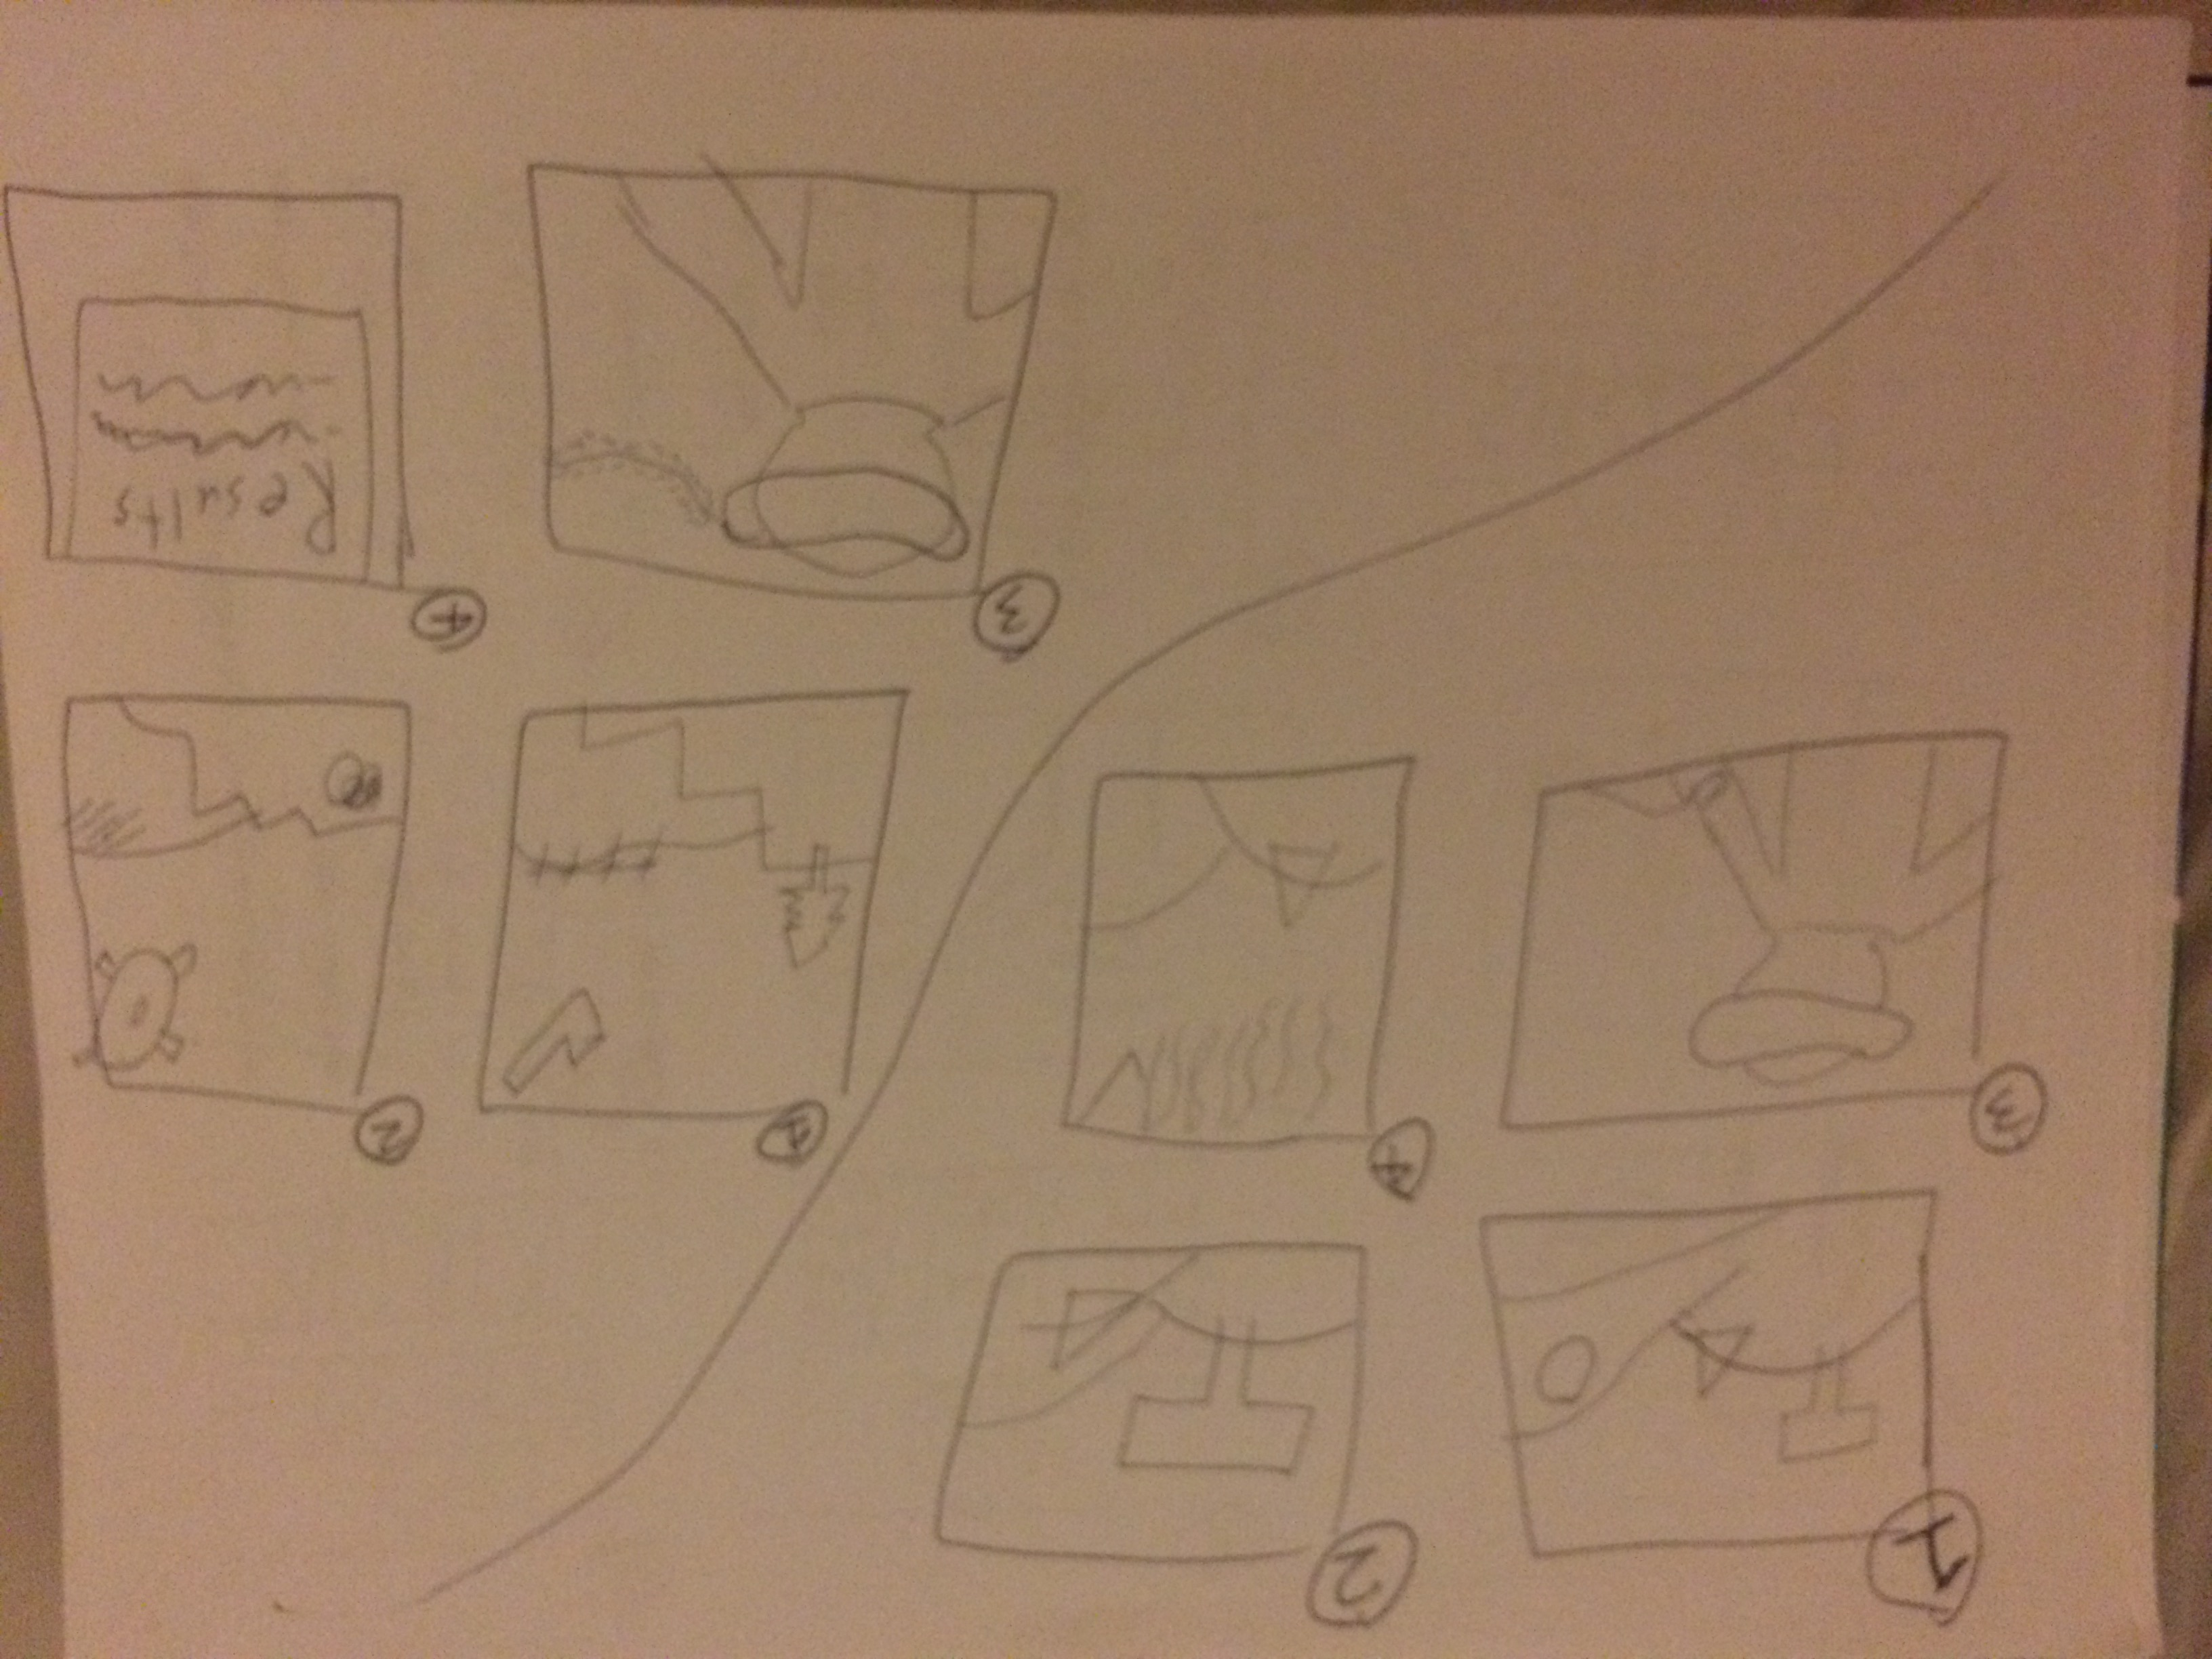
\includegraphics[scale = 0.13, angle = 180]{sbCalm.jpg}}
	\caption{Storyboard for Calming Module}
	\label{fig:elevator}
\end{figure}
\begin{enumerate}
	\item The program generates a procedurally generated enviroment
	\item The user can explore this enviroment, with quiet sounds and music sometimes being played.
	\item The program will check the user's stress level, and use this to check if the user is calm
	\item If the user is calm, the program will change the environment in small, subtle ways to reflect this, with a notification.
\end{enumerate}
\begin{enumerate}
	\item If the user enters the secondary mode, it will provide an obvious notification of if the user is calm
	\item If they are not calm, it will show them with the same obvious notification
	\item The user's relaxation level will be checked by the same sensors as indicated above
	\item A results page will be shown at the end with how well the user was able to remain calm.  This secondary mode is intended to help users learn to remain calm, not attempt to calm themselves down.
\end{enumerate}


\subsubsection{Design Concerns}
Our current plans are to include some premade plug-ins that generate terrains on the CPU with possibly some GPU acceleration, however we would like to try and generate our own terrain with Compute Shader provided in Unity.  Because the environment is abstract, it shouldn't require buying assets and should be easier to design.

\paragraph{Some factors that may limit our ability to do this include:}
\begin{itemize}
\item Access to some features related to direct pipeline which only comes with the Professional Version.
\item The efficiency of our generation and mapping algorithms on the GPU.
\item The already heavy load of meeting rendering demands of release level VR headsets which require a large frame buffer for two screens which each require different OpenGL rendering passes.
\item Most of these issues will be handled by Unity for most scenes but if we want to do any mapping on the fly we will have to meet these rendering/ processing time lines for our compute operations, 
and deal with the extra processing overhead for the GPU while making sure we can run the VR with decent settings and frame rates. 
\item We Will pick the best option for the terrain that provides the best immersion for the user and performance.
\end{itemize}
% https://scrawkblog.com/category/directcompute/
% http://answers.unity3d.com/questions/162096/gpu-programming-with-unity.html
\pagebreak
\subsubsection{GPGPU Research Outline}
Any generated terrain Unity supports compute shaders which are written in Direct X HLSL, and allow the application to do computations on the GPU for
these terrain calculations. These compute shaders allow the application to do most of the heavy computations on the GPU which provides massive speedups compared to the a CPU implementation.
\paragraph{This Section will discuss the following:}
\begin{itemize}
	\item GPU Overview 
	\begin{itemize}
		\item GPGPU Overview
		\item GPGPU processing model
		\item GPU Architecture
	\end{itemize}
	\item Unity Compute Shader/ GPU Processing Features
	\begin{itemize}
		\item Compute Shader Support
		\item Cross Platform Support
		\item Asynchronous Buffer Synchronization
		\item Unity Rendering Pipeline Features
		\item Advanced Compute Shader GPGPU Features
	\end{itemize}
	\item Overall Analysis On GPU Compute Shaders
\end{itemize}
\pagebreak
\subsubsection{General-purpose computing on graphics processing units (GPGPU)}
GPGPU programming is a growing option for parallel processing applications that work over large data sets. Some common uses include image or media processing and 
performing mathematical computations over linear systems or large sets. Many modern GPUs offer many benefits in processing with the high number of cores that can operate on data 
in Single Instruction Multiple Data (SIMD) and Multiple Instruction Multiple Data (MIMD) fashions. For example, one group of data can be processed with the same instruction in parallel 
and the GPU can have multiple groups scheduled at the same time. The basic unit of execution on a GPU (the compute shader or kernel) is run in parallel and scheduled by the GPU execution context
and the commands are setup and issued by the cpu application in a queue fashion, some execution can be synced to wait for other kernels to complete or can be dispatched and run in whatever order.


\paragraph{Explanation of GPGPU Processing Models}
The most basic unit of Processing on a GPU is work item (AMD) or thread (NVIDIA) this represents a single piece of data that is processed in parallel. Most GPUs organize these processors in groups called 
compute units which are controlled by a scheduler to process data in blocks on each compute unit. For an example such as modifying the pixel values of an image, each compute unit takes a part of the image 
and process it until the entire image is finished. The dimensions of the entire workload are set as a parameter to the GPU giving it the total number of elements to process as an N-Dimensional range (right 
now most GPUs go up to 3 Dimensions). This global size is then divided up by a work group size, and the work groups are then processed by the compute units \textbf{ (see figure \ref{fig:gpu})}. The dimensions of these work groups 
can be modified to optimize for different algorithms depending on how they access data. 
	\begin{figure}[H]
	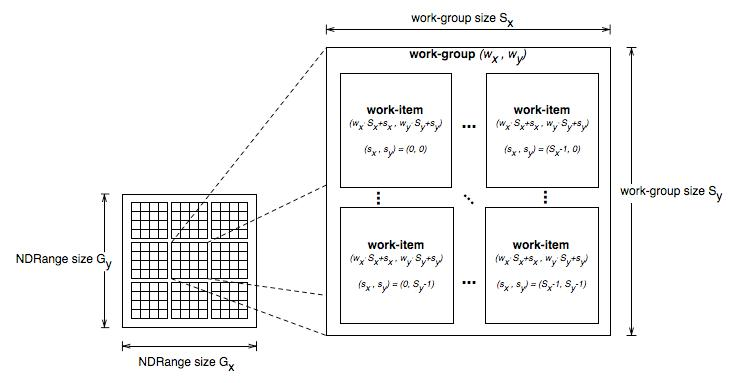
\includegraphics[width=\linewidth,height=\paperheight,keepaspectratio]{gpgpu.jpg}
	\caption{GPGPU Diagram}
	%Figure \ref{fig:gpgpuImg} shows our blockDiagram.
	\label{fig:gpu}
	\end{figure}
\pagebreak

\subsubsection{GPU Architecture Overview}
\paragraph{Specific designs of compute units can vary between GPUs but common components include:}
\begin{itemize}
\item Large groups of SIMD processors with separate private memory (registers) 
\item Local memory that is shared between the processors on a compute unit
\item Specialized components for pixel/texture operations such as rasterization
\item Global memory components such as a L1 cache (on the compute unit) and L2 cache that is accessible globally for all compute units.
\item Figure \ref{fig:gpuArch} shows an example compute unit design and Figure \ref{fig:gpuMem} shows the general memory model pattern.
\end{itemize}
	\begin{figure}[H]
	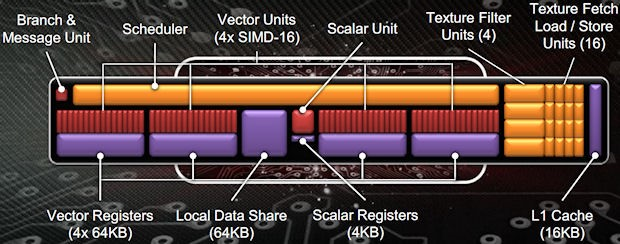
\includegraphics[width=\linewidth,height=\paperheight,keepaspectratio]{gpuArch.jpg}
	\caption{GPU Architecture Diagram}
	%Figure \ref{fig:gpgpuImg} shows our blockDiagram.
	\label{fig:gpuArch}
	\end{figure}
	
	\begin{figure}[H]
	\centerline{ 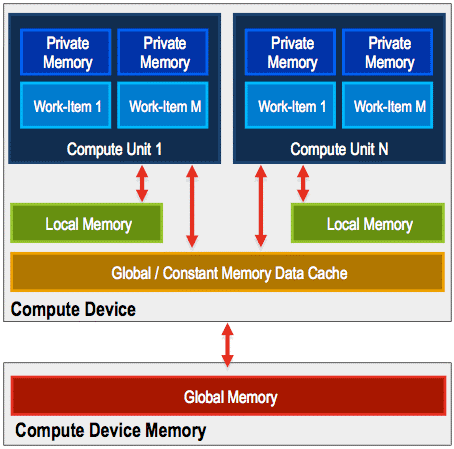
\includegraphics[scale=0.5]{gpuMem.png}}
	\caption{GPU Memory Diagram}
	%Figure \ref{fig:gpgpuImg} shows our blockDiagram.
	\label{fig:gpuMem}
	\end{figure}
\pagebreak



\subsubsection{Unity Support for Asynchronous Compute Shaders and Kenrels}
\paragraph{Shading Languages used in Unity} 
In Unity, shader programs are written in a variant of HLSL language (also called Cg but for most practical uses the two are the same). Unity recommends developers have a good understanding 
of OpencL Or CUDA, OpenGL, and other Graphics/ GPGPU parallel compute languages.  

Internally, different shader compilers are used for shader program compilation:\cite{unityShaders}
\begin{itemize}
  \item Windows and Microsoft platforms (DX9, DX11, DX12, XboxOne and Xbox 360 ) all use Microsoft's HLSL compiler.
  \item OpenGL Core (GL3) and OpenGL ES 3 use Microsoft’s HLSL followed by bytecode translation into GLSL, using a modified version of hlslcc.
  \item OpenGL Legacy (GL2), OpenGL ES 2.0 and Metal use source level 
  translation via
  hlsl- 2glslfork and glsl optimizer. 
  \item Other console platforms use their respective compilers (e.g. PSSL on PS4).
  \item Surface Shaders use Cg 2.2 and MojoShader for code generation analysis step.
\end{itemize} %unity ref http://docs.unity3d.com/Manual/SL-ShadingLanguage.html
\subsubsection{Unity Cross Platform Shader Support (Android)}
In order to achieve shaders working on multiple different platforms one should consider these limitations:\cite{unityXP}

\begin{itemize}
\item 
D3D and OpenGL have different data layout rules. Automatically translated GLSL shaders use std430 layout on compute buffers. Therefore for example using float3 based structured buffers will cause compatibility issues as DX allows tight packing but OpenGL enforces padding to float4. Scalars, two-component and four-component vectors are safe to use as they are. Extra care should be taken when constructing structs.
\item 
OpenGL ES 3.1 guarantees support for only 4 simultaneous shader storage buffers. Actual implementations typically support a bit more but in general one should consider grouping related data in structs as opposed to having each data item in its own buffer.
HLSL-only or GLSL-only compute shaders

\end{itemize}

Typically compute shader files are written in HLSL, and compiled or translated into all needed platforms automatically. However it is possible to either prevent translation to GLSL (i.e. only keep HLSL platforms), or to write GLSL compute code manually.
\begin{itemize}
\item Compute shader source surrounded by CGPROGRAM and ENDCG keywords will not be processed for OpenGL/GLSL platforms.
\item Compute shader source surrounded by GLSLPROGRAM and ENDGLSL keywords will be treated as GLSL source, and emitted verbatim. This will only work when targetting OpenGL/GLSL platforms.
\end{itemize}
\pagebreak

\subsubsection{Unity Support for Graphics Asset Related Operations}
One of the common bottlenecks in GPGPU processing is buffer transfer to the GPU memory before processing, Unity allows asynchronous texture uploads to allow the application to time slice the GPU resources to upload textures or other assets to the device, this means that it will take longer overall time to do transfer assets but if scheduled properly the background expected algorithms that need specific buffers should not have to block on the buffer transfers.
\begin{figure}[H]
	\centerline{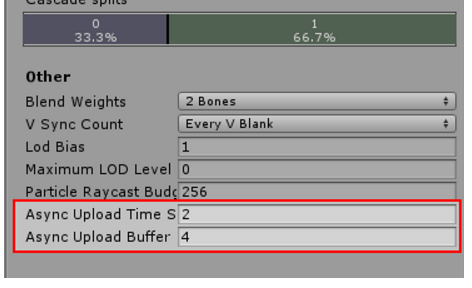
\includegraphics[scale= 0.75]{asychTexture.png}}
	\begin{itemize}
\item Upload time: Amount of time (ms) spent on asynchronous uploads per frame.
\item Upload Buffer: Size of texture upload buffer in MB unity usually adjusts this automatically but it can be set by the application.
\end{itemize}
	\caption{Unity Asynch Texture Options}
	%Figure \ref{fig:gpgpuImg} shows our blockDiagram.
	\label{fig:gpuTex}
	\end{figure}

\paragraph{Guarantees and Restrictions} 
For non-read/write enabled textures, the Texture Data is part of resS (Streaming Resource) and upload now happens on Render-Thread. Availability of Texture is guaranteed during call to AwakeFromLoad. (This only works for textures or buffers that are not used in any custom processing.)\cite{unityAsynch}
~\\
For other types of texture loading, such as read/write enabled textures, textures loaded directly with the LoadImage(byte[] data) function, or loading from the Resources folder, the Asynchronous buffer loading is not used - the older Synchronous method is used.
These restrictions mean that we will have to schedule and synchronize the transfer of any custom textures or buffers to and from the GPU.
In order to avoid all of the transfer penalties the frequency, size, and amount of transfers should be minimized, and all the major assets should be kept on the GPU.

\pagebreak


\subsubsection{Unity Camera Rendering Pipeline}
Unity supports the exposes the command buffer which is similar to the main rendering pipeline in most graphics processing frameworks (OpenGL's paint or render loop, OpenCL's command queue etc.) This framework supports blitting, drawing meshes, drawing procedural geometry (compute shaders), and many other common graphics drawing features. \textbf{(See Figure \ref{fig:gpuPipe})} %NEEDS WORK blitting?

\begin{figure}[H]
	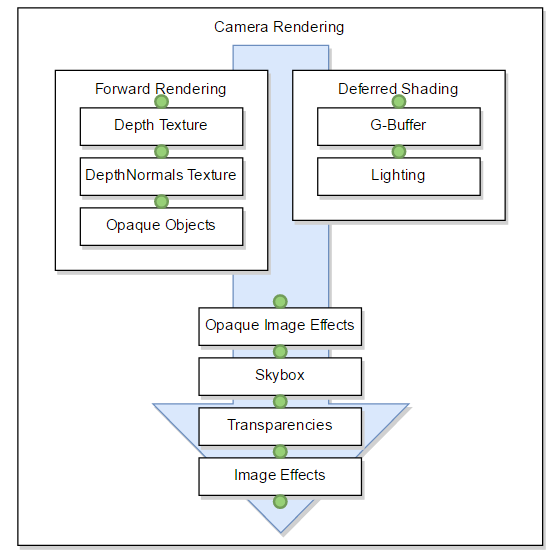
\includegraphics[width=\linewidth,height=\paperheight,keepaspectratio]{cameraRender.png}
	\caption{Unity Command Buffer Camera Pipeline}
	%Figure \ref{fig:gpgpuImg} shows our blockDiagram.
	\label{fig:gpuPipe}
	\end{figure}

\pagebreak

\subsubsection{Advanced GPGPU features}
% try unity zip in google drive with atomic and local mem barriers
Some advanced GPGPU related constructs useful for highly optimized compute 
processing, need to be checked if they are included in Unity's implementation of Direct Compute,which 
is similar to the HLSL code snippets listed below.
\paragraph{Shared Memory Reduction Kernel}
\begin{figure}[H]
	\label{fig:reductionCode}
\lstinputlisting [language =C] {shared_mem_reduction.hlsl}
\caption{Reduction Code}
\end{figure}

This kernel is a Compute Shader that is run on the GPU and allows for synchronization of shared memory across multiple compute units, this technique is useful for parallel reduction algorithms which include
calculations such as min, max, mean, sum etc... anything that can be reduced to simpler worksets are are not iterative in nature. \textbf{(see figure \ref{fig:reductionImg})}

\begin{figure}[H]
	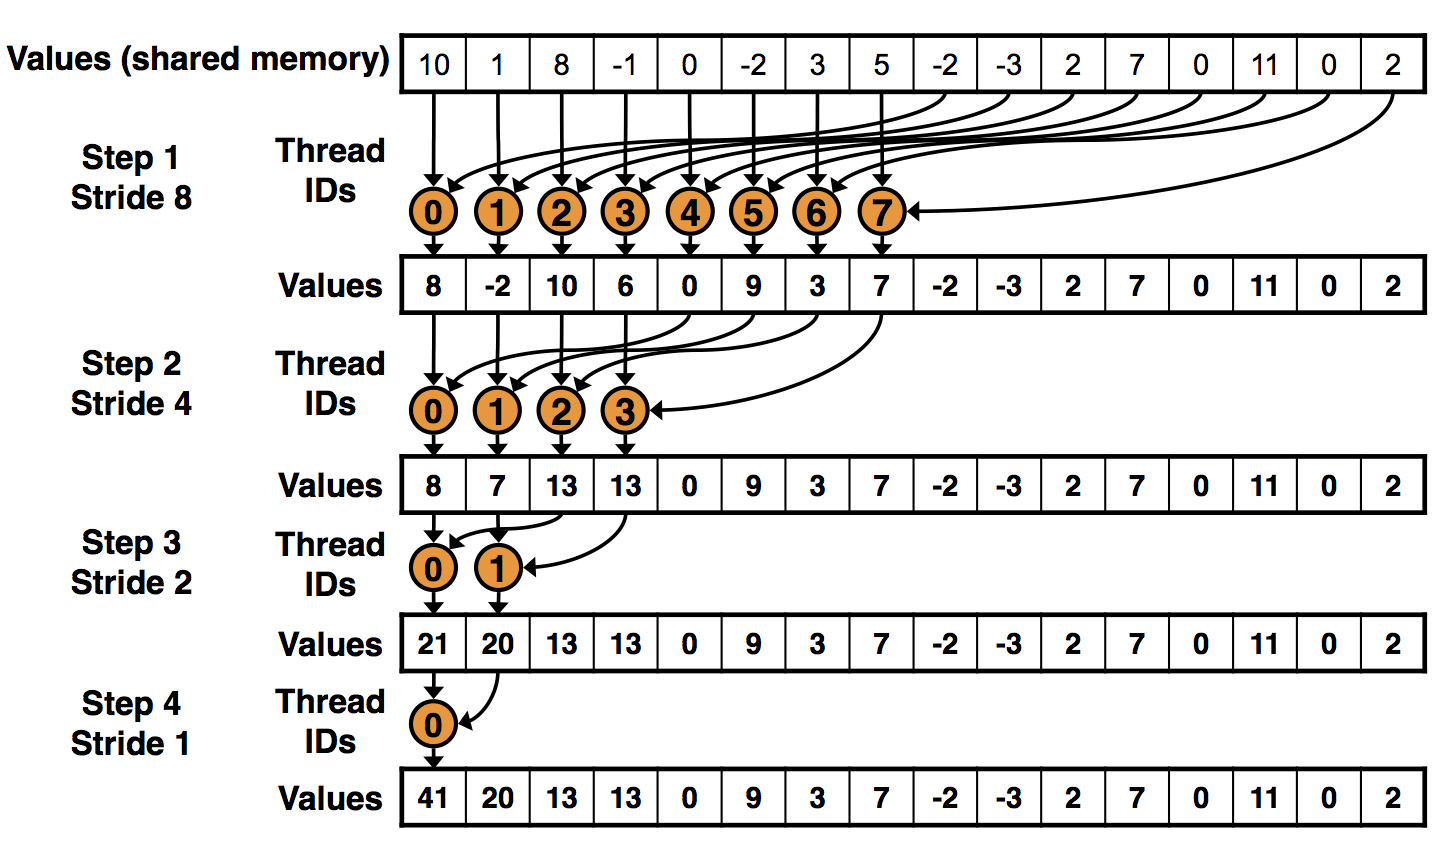
\includegraphics[width=\linewidth,height=\paperheight,keepaspectratio]{reduction.jpg}
	\caption{Reduction Diagram}
	%Figure \ref{fig:gpgpuImg} shows our blockDiagram.
	\label{fig:reductionImg}
	\end{figure}
\paragraph{Shader Processor Atomics} 
This is another powerful feature that is supported in Unity Compute shaders, it creates atomic accesses for compute units and shader processors which allow the kernels to avoid race conditions. 
\begin{figure}[H]
\lstinputlisting [language =C] {atomic_inc.hlsl} %NEEDS WORK math call error?
This kernel is a compute shader that is run on the GPU and allows for synchronization adding or various operations that are done in an atomic fashion, avoiding, race conditions.
\caption{Atomic Code}
%Figure \ref{fig:gpgpuImg} shows our blockDiagram.
\label{fig:atomicCode}
\end{figure}

\pagebreak
%E. Explicit Design Summary with diagrams
%F. Build, prototype, test, and evaluation plan
\section{Design Documentation}
	\subsection{Block Diagrams:}
	\begin{figure}[H]
	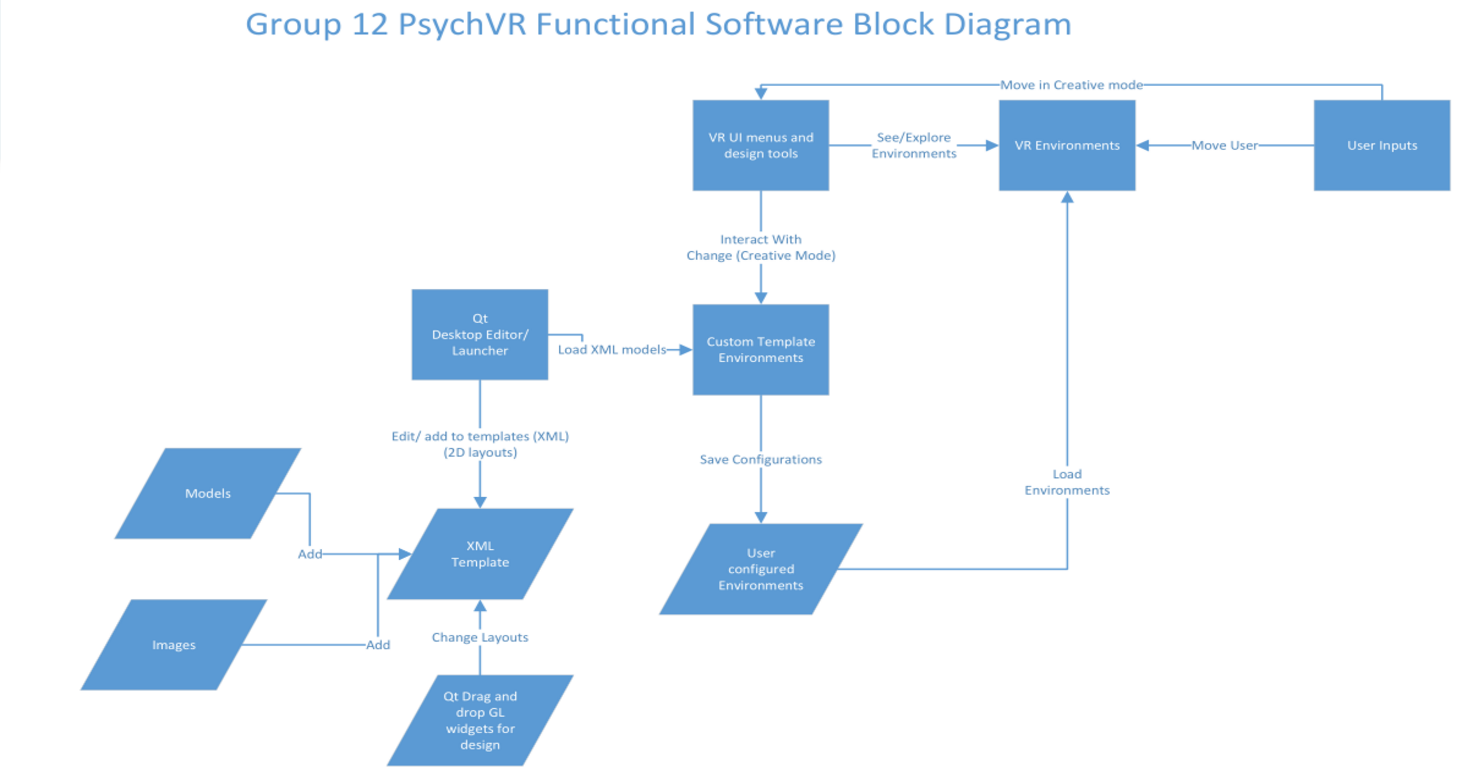
\includegraphics[width=\linewidth,height=\paperheight,keepaspectratio]{HardwareConfig.png}
	\caption{Hardware Block Diagram}
	%to ref fig number
	%Figure \ref{fig:block1} shows our blockDiagram.
	\label{fig:hblock}
	\end{figure}
	This diagram represents a hardware configuration of a typical VR system that our application would expect. This may change depending on the device we use, but is a good overview.
	\pagebreak
	\begin{figure}[H]
	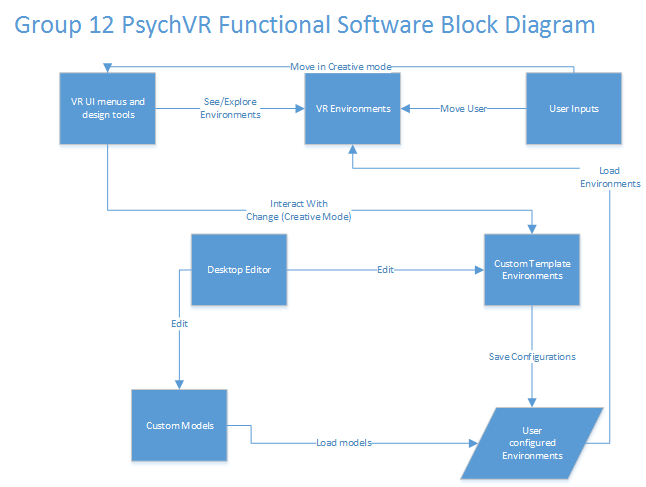
\includegraphics[width=\linewidth,height=\paperheight,keepaspectratio]{SoftwareConfig.png}
	\caption{Software Block Diagram}
	%to ref fig number
	%Figure \ref{fig:block2} shows our blockDiagram.
	\label{fig:sblock}
	\end{figure}
	This diagram represents the software design of our project and the various functional modules that should exist in order to fulfill the user interaction requirements. 
	The application will have two main modes of operation, edit mode and view mode. 
	\subsection{Overall High Level Design}
		\begin{figure}[H]
			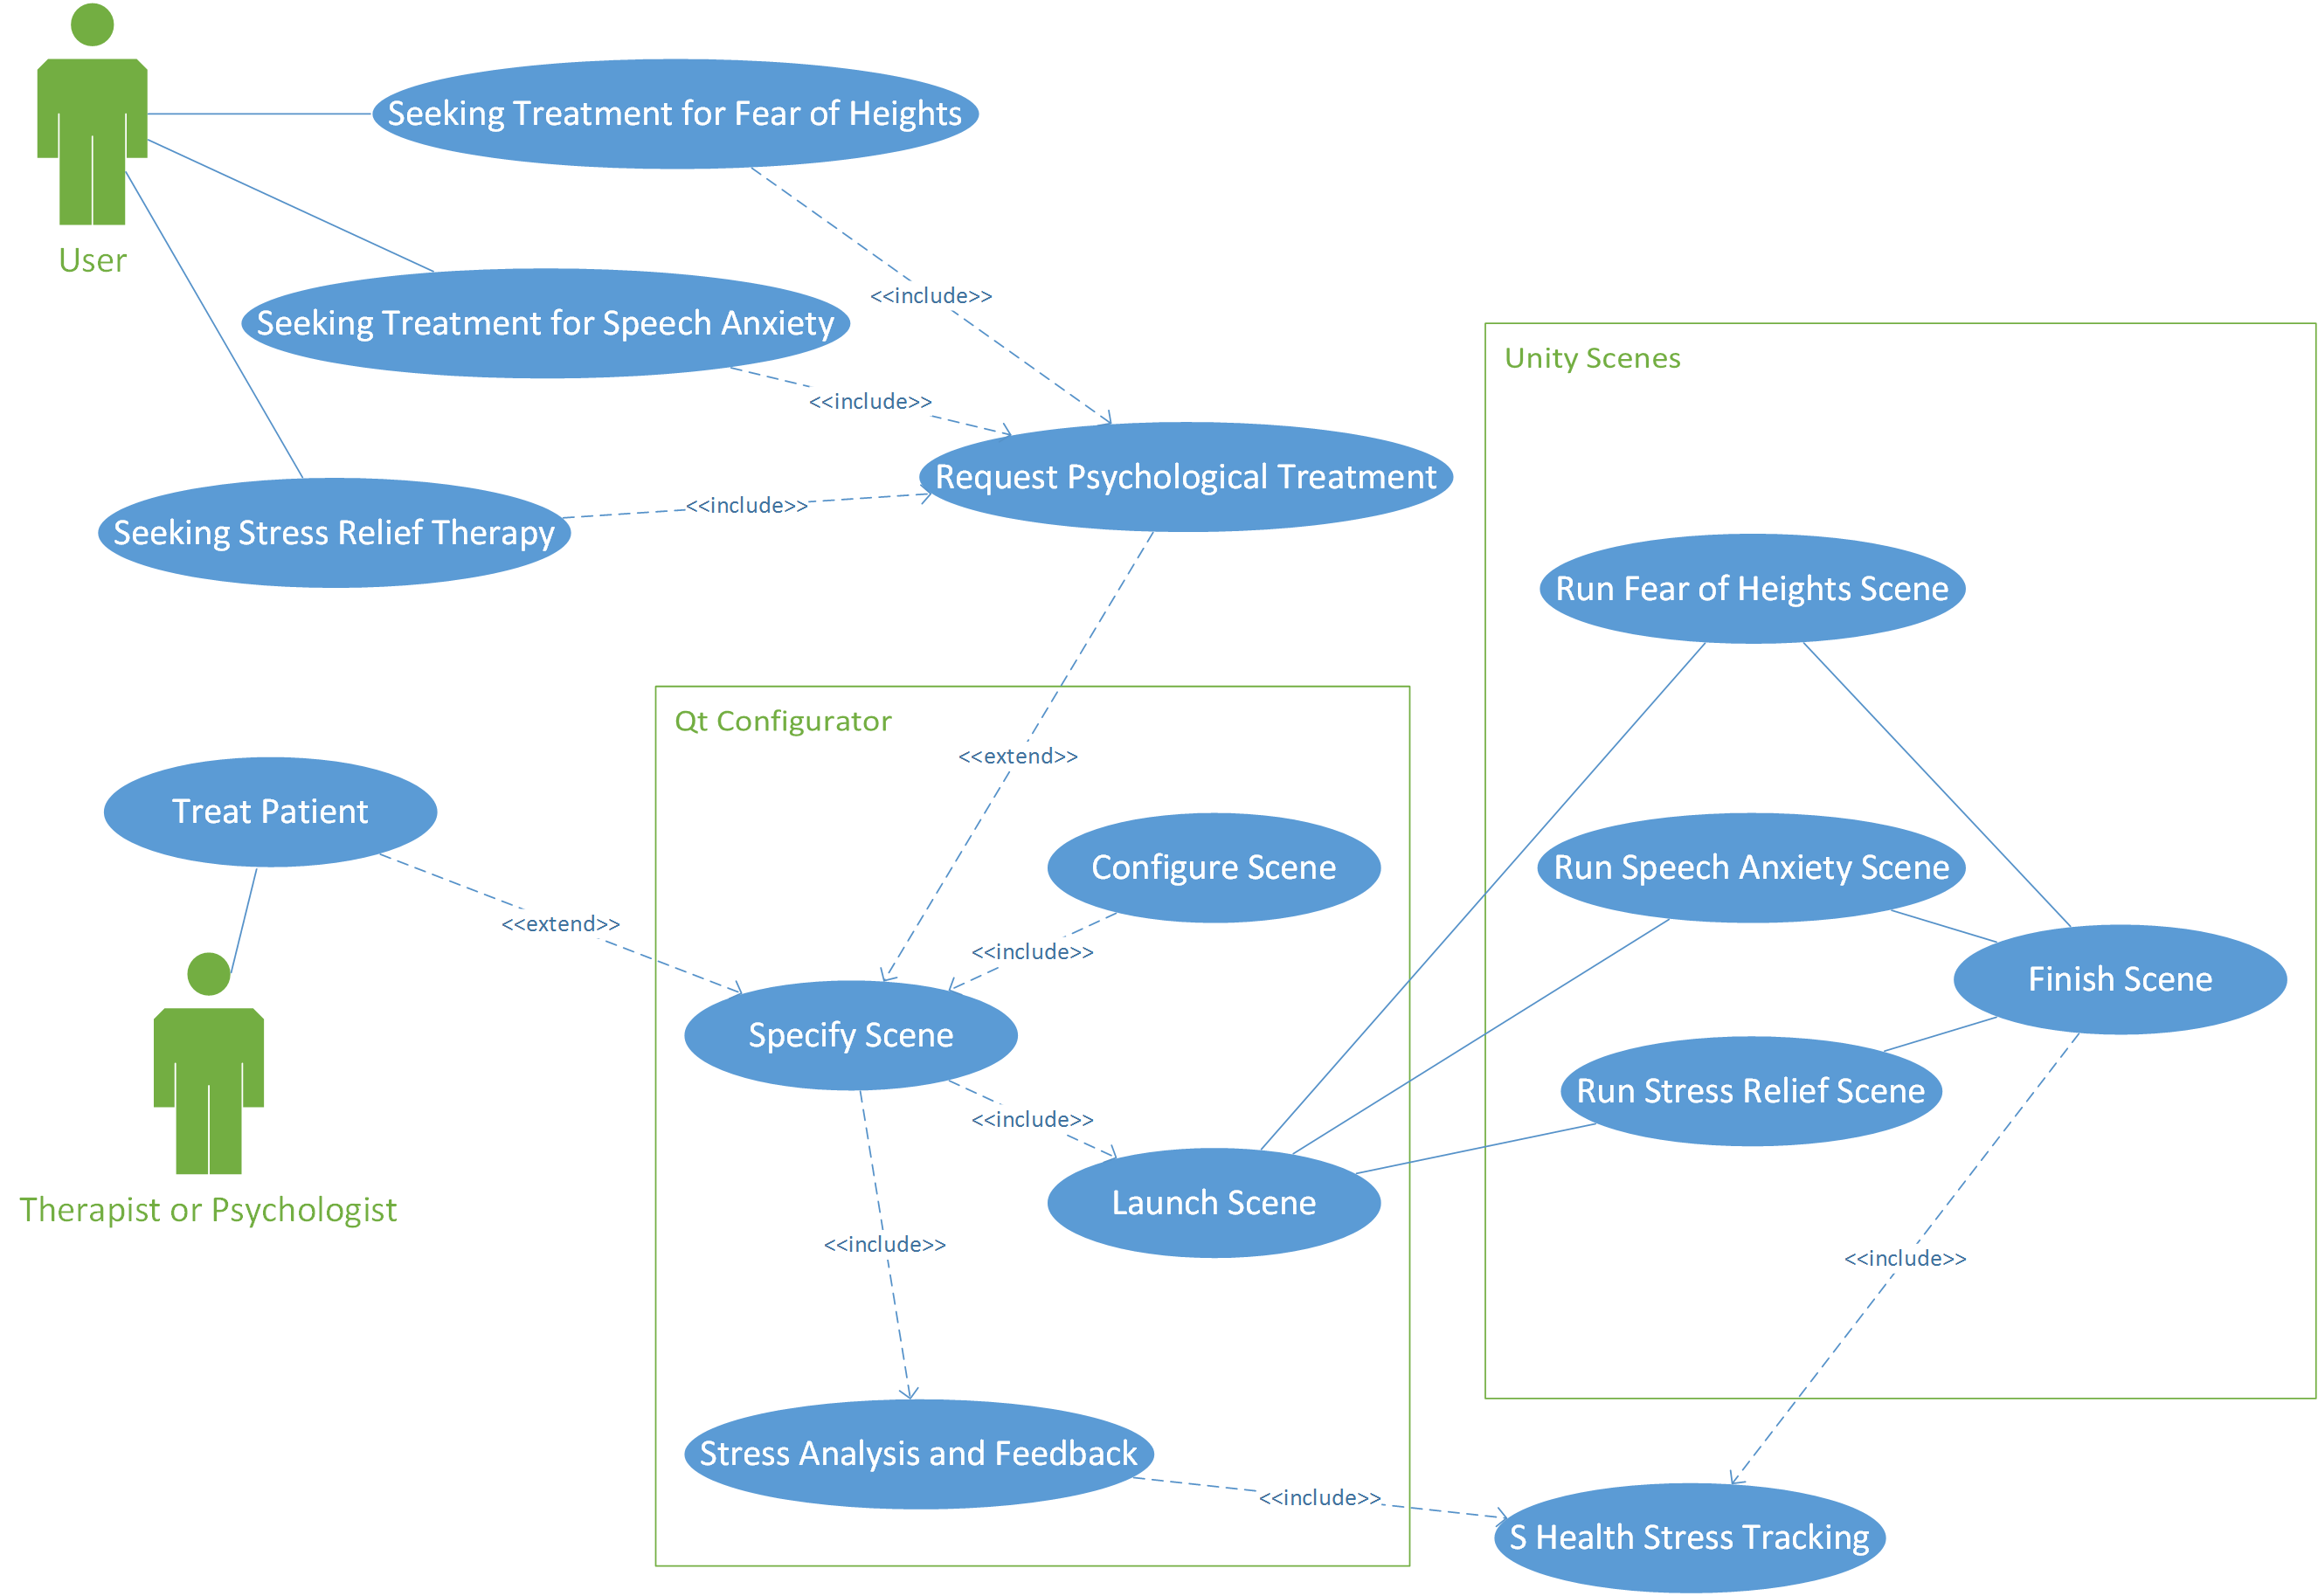
\includegraphics[width=\linewidth,height=\paperheight,keepaspectratio]{highUseCase.png}
			\caption{High Level Use Case Diagram}
			%to ref fig number
			%Figure \ref{fig:block2} shows our blockDiagram.
			\label{fig:highlevelusecase}
		\end{figure}
		This Figure represents the general use case and standard user interactions. It also includes some optional parts that are related to the therapy and treatment which 
		may or may not involve a psychologist. Users at home will have the ability to run configure scenes, and review stress and other analysis data, Psychologists can also use
		the tool as a therapy option and can use the stress and analysis as feedback.
	\pagebreak
	\subsection{Qt Design Plan}
		\subsubsection{Qt High Level Diagram}
		\begin{figure}[H]
					\includegraphics[width=\linewidth,height=\paperheight,keepaspectratio]{qtConfigDiag.png}
					\caption{Qt Design Diagram}
					%to ref fig number
					%Figure \ref{fig:block2} shows our blockDiagram.
					\label{fig:qtHighLevel}
				\end{figure}
This figure shows the general design for the Qt Configuration Tool/ Launcher. This launcher will be the main editing/ 
configuration option for the app, It will also be responsible for launching scenes, scene settings and configuration, and graphing user stress data.

		\pagebreak
\subsubsection{Qt Activity Diagram}
		\begin{figure}[H]
			\includegraphics[width=\linewidth,height=\paperheight,keepaspectratio]{qtActivityDiag.png}
			\caption{Qt Activity Diagram} 
			
			%to ref fig number
			%Figure \ref{fig:block2} shows our blockDiagram.
			\label{fig:qtactivity}
		\end{figure}
		This figure shows the program flow for different user options, including configuration, launching, recording, and vie
		\pagebreak

\subsubsection {Configuration Design Details}
(See figure \ref{fig:qtMockupMap})
\begin{itemize}
\item Users can Select the scene to edit the configurations, with the set scene options we have added, new scenes could be added to the dropdown if new scenes were created.
\item Configurations will be saved to a specific .ini or settings file that will be parsed by the unity scene on load.
\item Basic settings such as resolution, quality options, and other static options will be in dialog boxes.
\item The scene maps will be encoded with some options including size, the list of available models with names(ex desks, trees, etc.), and other available settings for scenes, this file will be read in by Qt and setup the configuration options for the user.
\item The Graphics view (Map Viewer)will allow the user to drag and drop models UnityObjects(CUnityObject) from the list on the scene and move them around. %NEEDS WORK?
\item Any previously saved configurations be loaded and UnityObjects will be shown in the Map Viewer.
\item The configuration can be saved and will be used to launch the app.

\end{itemize}
\begin{figure}[H]
				      \centerline{\includegraphics[scale = 0.35]{qtConfigMap.png}}
					\caption{Qt Design Mock-up}
					%to ref fig number
					%Figure \ref{fig:block2} shows our blockDiagram.
					\label{fig:qtMockupMap}
				\end{figure}
\pagebreak
\subsubsection{Data Analysis Design}
(See figure \ref{fig:qtMockupData})
  \begin{itemize}
  \item User stress data from Samsung stress app on (acquired from android phone or another input device will be parsed and graphed in the OpenGL Graph widget.
  \item Any other analysis will be shown as dialog boxes or additional readouts next to the graph.
  \item Input Options include reading from the android sensor DataManager app which allows users to export their stress data to a csv, or the user can input their stress readings
  from the Samsung Health app manually which ever requires the least installation, setup, or amount of work each time for the user which we will see which option is easier from a human 
  factors standpoint.
  \item Other Scene specific data could also be recorded and graphed to provide additional feedback some examples for the specific modules include:
	\begin{itemize}
	\item Distance moved or time spent in fear of heights session.
	\item Speech Gestures, rate or word recognition with speech anxiety session.
	\item Distance covered or movement data from stress relief sessions.
	\end{itemize}
\item All of these graph options could be selectable as options for each scene graph widget and would be subclassed accordingly.
  \end{itemize}
\begin{figure}[H]
				      \centerline{\includegraphics[scale = 0.35]{qtConfigData.png}}
					\caption{Qt Design Mock-up}
					%to ref fig number
					%Figure \ref{fig:block2} shows our blockDiagram.
					\label{fig:qtMockupData}
				\end{figure}

\pagebreak
	\subsection{Unity Design Plan}
		\subsubsection{Unity High Level Design}
		\begin{figure}[H]
					\centerline{\includegraphics[]{UnityHighlevel.png}}
					\caption{Unity High Level Design Diagram}
					%to ref fig number
					%Figure \ref{fig:block2} shows our blockDiagram.
					\label{fig:unitydesign}
				\end{figure}
				
		\pagebreak
		\subsubsection{Unity Activity Diagram}
				\begin{figure}[H]
					\centerline{\includegraphics[]{unityActivityDiag.png}}
					\caption{Unity Activity Diagram}
					%to ref fig number
					%Figure \ref{fig:block2} shows our blockDiagram.
					\label{fig:unityactivity}
				\end{figure}
				\pagebreak
		\subsubsection{Unity Design Details}	
\begin{itemize}
	\item Configurable scenes are going to initially read an expected Qt configuration file that 
	will contain scene specific settings and include any additional models added to the scene mapped 
	by the mapping tool. 
	\item The Kinect camera, Oculus Rift, and Leap motion will be added as input controls mapped to a first person avatar that has is own models and textures for hands, legs, arms and body. 
	\item The scene models will have interactive scripts that will interact with the user such as doors, or other objects they can move or pick up. 
	\item Models and scene assets that can be configured will be written to a QtConfigFormatFile which will be parsed by Qt to get icons, sizes, and names of the CUnityObject class models that can be configured. 
	\item The settings will be stored as QSettings objects from Qt which will store them as a .ini file which is supported by unity and will allow the two applications to synchronize options by parsing the .ini files on load. 
	\item Unity assets will be purchased in the asset store or designed in Google SketchUp \& Blender then imported. 
\begin{figure}[H]
	\label{fig:sceneTemplate}
\lstinputlisting {test.ini}
\caption{Example scene template file}
\end{figure}
\end{itemize}	
		\pagebreak
		%\subsubsection{Scene Shared Assets}
		\subsubsection{Survey High Level Design}
			\begin{figure}[H]
					\centerline{\includegraphics[]{survey.png}}
					\caption{Survey High Level Diagram}
					%to ref fig number
					%Figure \ref{fig:block2} shows our blockDiagram.
					\label{fig:surveyDiag}
				\end{figure}
				This diagram represents an option for our survey design for gathering user stress feedback. It will ask the user a set series of questions to determine their stress level.
\pagebreak

\subsubsection{Fear of Heights Activity Diagram}
\begin{figure}[H]
					\centerline{\includegraphics[scale = 0.6]{fohActivityDiag.png}}
					\caption{Fear of Heights Activity Diagram}
					%to ref fig number
					%Figure \ref{fig:block2} shows our blockDiagram.
					\label{fig:fohAct}
				\end{figure}
\subsubsection{Speech Anxiety Activity Diagram}
\begin{figure}[H]
					\centerline{\includegraphics[scale = 0.6]{spcActivityDiag.png}}
					\caption{Speech Anxiety  Activity Diagram}
					%to ref fig number
					%Figure \ref{fig:block2} shows our blockDiagram.
					\label{fig:spcAct}
				\end{figure}
\subsubsection{Stress Relief Activity Diagram}
\begin{figure}[H]
					\centerline{\includegraphics[scale = 0.8]{stressActivityDiag.png}}
					\caption{Stress Relief Activity Diagram}
					%to ref fig number
					%Figure \ref{fig:block2} shows our blockDiagram.
					\label{fig:stressAct}
				\end{figure}
				\pagebreak
\subsection{Integration Setup}

These are the hardware/ development environment setup instructions. 
\begin{itemize}
 \item Install Instructions:
 \begin{itemize}
 \item  Getting Binaries: Download from github
  \item Install the Oculus Rift Home Drivers: Download the drivers from~\\ \url{https://www.oculus.com/en-us/setup/}
  \item Install the Leap Motion Drivers: https://developer.leapmotion.com/get-started
  \item Install the Kinect For Windows Drivers: ~\\\url{https://www.microsoft.com/en-us/download/details.aspx?id=44559}
 \end{itemize}
 \item Development Instructions:
  \begin{itemize}
   \item Getting our software: These instructions assume you have already installed the hardware system device drivers 
listed in the Install section.
\item Install Qt:
Our Project uses Qt Creator 3.6.1 Based on Qt 5.6.0. Community (Opensource Version) 
it can be installed from ~\\\url{https://www.qt.io/download-open-source/}
For help with installation or more detailed instructions see
http://doc.qt.io/qt-5/gettingstarted.html 
\item Install Unity:
Our Project uses Unity 5.3.4 
it can be installed from 
~\\\url{https://unity3d.com/unity/whats-new/unity-5.3.4}
For help with installation or more detailed instructions see
~\\\url{http://docs.unity3d.com/Manual/InstallingUnity.html}
\item Oculus Rift SDK:
https://developer.oculus.com/downloads/
This download page includes many examples and tutorials
\item Leap Motion SDK:
https://developer.leapmotion.com/get-started
For more details on Using Leap with Unity ~\\\url{https://developer.leapmotion.com/unity} 
\item Kinect SDK:
~\\\url{https://www.microsoft.com/en-us/download/details.aspx?id=44561}
For more information on setup and development  ~\\\url{https://developer.microsoft.com/en-us/windows/kinect}
Cross Platform Support:

  \end{itemize}
  \item Cross Platform Development
  As much as we would like to have full cross platform support for this app, As of right now 
  Oculus Home is only supported on Windows if other OS support 
  is added or another VR device is used development for building to other operating systems or
  implementing other headsets should be simple.
  \begin{itemize}
  \item Qt is designed to be cross platformm. 
  \item Leap Motion is already cross platform unless the orion driver is needed
  ~\\\url{https://developer.leapmotion.com/get-started}
    \item OpenKinect is an Opensource project that supports C\#.
  \url{https://openkinect.org/wiki/CSharp_Wrapper}
  \item Unity Scenes Build cross platform, just download Binaries.\
  \item Also Unity is cross platform as an experimental version.
  \end{itemize}
\end{itemize}
\pagebreak
\subsection{Test Plan}
\subsubsection{Functional Tests}
\begin{enumerate}
    \item  Qt Launcher Functionality
    \begin{itemize}
	\item Test Objective: Check that Unity Scenes can be launched by the Qt app.
	\item Test Description: Make sure scene is loaded and correct scene is launched.
	\item Test Conditions: The user selects a scene and presses the launch button
	\item Expected Results: The user should be able to launch the scene they select.
    \end{itemize}
     \item  Qt Save/Load Configuration File
    \begin{itemize}
	\item Test Objective: Check that Unity Scenes configurations can be loaded by the Qt app.
	\item Test Description: Check that the configuration options can be saved and loaded
	\item Test Conditions: The user loads or saves a file. 
	\item Expected Results: The configuration options should be persistent.
    \end{itemize}
     \item  Qt Data Measurement
     \begin{itemize}
	\item Test Objective: Check Qt records or reads some acquired stress or scene related data.
	\item Test Description: Check that this data is recorded.
	\item Test Conditions: Use a scene, record data.
	\item Expected Results: The data should  be recorded.
    \end{itemize}
    \item  Unity Data Measurement
     \begin{itemize}
	\item Test Objective: Check Unity records or reads some acquired stress or scene related data.
	\item Test Description: Check that this data is recorded.
	\item Test Conditions: Use a scene, record data.
	\item Expected Results: The data should  be recorded.
    \end{itemize}
    \item  Qt Data Analysis
     \begin{itemize}
	\item Test Objective: Check Qt analyzes or graphs some acquired stress or scene related data.
	\item Test Description: Check that this data is analyzed or graphed.
	\item Test Conditions: Use a scene, record data, check graph or analysis.
	\item Expected Results: The data should  be analyzed or graphed.
    \end{itemize}
     \item Kinect Movement Tracking
     \begin{itemize}
	\item Test Objective: Check that user Kinect movement and gesture tracking works
	\item Test Description: Kinect movement and Skeleton tracking should allow the user to move aroud the scene and the system should be able to track gestures.
	\item Test Conditions: Use a scene, verify that the user can move.
	\item Expected Results: The user movements should be fluid and accurate.
    \end{itemize}
     \item Leap Motion Tracking
     \begin{itemize}
	\item Test Objective: Check that user Leap Motion hand movement and gesture tracking works
	\item Test Description: Leap Motion should allow the user to be able to interact with their hands.
	\item Test Conditions: Use a scene, verify that the user can move their hands.
	\item Expected Results: The hand movements should be fluid and accurate.
    \end{itemize}
     \item Oculus Rift Motion Tracking
     \begin{itemize}
	\item Test Objective: The User's view/ head orientation should turn with the Rift.
	\item Test Description: Oculus gyroscopes and sensors should allow rotation.
	\item Test Conditions: Use a scene, verify that the user can rotate their view.
	\item Expected Results: The rotation should be fluid and accurate.
    \end{itemize}
     
\end{enumerate}

\subsubsection{Module Specific tests}
\begin{enumerate}
    \item  Fear of Heights Usability
     \begin{itemize}
	\item Test Objective: Check The fear of heights scene is usable.
	\item Test Description: The scene should be realistic, interactive, and run well, the user should be immersed in 
	the scene and should experience some believable stress or immersion in the scene.
	\item Test Conditions: Use this scene, verify that it is usable.
	\item Expected Results: The scene should meet these standards.
    \end{itemize}
    \item  Speech Anxiety Usability
     \begin{itemize}
	\item Test Objective: Check The speech anxiety  scene is usable.
	\item Test Description: The user should be put in a presentation or interaction where they feel some immersion to speaking in front of an audience.
	\item Test Conditions: Use this scene, verify that it is usable.
	\item Expected Results: The scene should meet these standards.
    \end{itemize}
    \item  Stress Relief Usability
     \begin{itemize}
	\item Test Objective: Check The stress relief scene is usable.
	\item Test Description: The user should be put in a calming peaceful environment that they can interact with.
	\item Test Conditions: Use this scene, verify that it is usable.
	\item Expected Results: The scene should meet these standards.
    \end{itemize}
    

\end{enumerate}
\pagebreak

%4. Administrative content
%G. Personnel and bibliography of related work, if any (mostly text)
%H. Facilities and Equipment (text, numbers, tables, charts, figures, diagrams)
%I. Consultants, subcontractors, and suppliers (mostly text)
%A. Budget and financing (text, numbers, tables, charts, figures, diagrams).
%B. Milestone chart for all activities related to the project
\section{Administrative Content}
\subsection{Budget and Financing}
Financing is still being looked into at this point. Due to our lack of a sponsor, we are currently self-financing but also contacting people willing to help with funding. Therefore, our budget and financing are extremely subject to change. 
\par~\\ 
We already have the hardware necessary to run virtual reality devices, so that saves us the cost of building one ourselves which can run upwards of \$1000. VR headsets vary in price, although our current target, the Oculus Rift DK2, costs 600 dollars. We have already acquired an Oculus Rift DK1 from the psychology department at no cost.
\par~\\ 
Using Unity Pro runs 75 dollars a month, so over the next 8 months it would add up to another 600 dollars. This can be ignored though since our research has found that we can accomplish our design goals without the pro features of Unity.
\par~\\ 
Our next greatest cost will be Unity Asset Store models, animations, and environments. Because designing models and creating animations is very time consuming, purchasing these assets is our best option. Our research on the models and environments we will need puts us at a maximum of \$400 in asset store costs for the highest quality options.
\par~\\
Peripherals will also need to be factored in. Leap Motion costs \$60 for the controller so we can detect hand gestures. Kinect will cost another \$60-\$120 so we can include more advanced motion tracking than simply head tracking.
\par~\\ 
Additionally, if we find a sponsor or funding from UCF, we can increase our budget and invest in higher end VR technology, and possibly be able to test for multiple platforms. A number of on campus facilities have alternatives to the Oculus Rift such as Sony’s VR headset Morpheus. The upper limit of our goals would be the HTC Vive with better motion tracking and controls at a cost of \$800. The benefit of this would be bringing our project to a wider audience.

\subsection{Summary:}
Current Budget: Approx. \$1000.  
\begin{itemize}
	\item \$400-600 for Oculus DK2, we have acquired a DK1 from the psychology department but would like to use a device with a higher frame rate, resolution, and other features to make the tests more immersive (See Section \ref{section:headset} for more details)
	\item  \st{\$600 for development Engine, (Unity Professional) we would only need this if we go with custom compute shaders and find that we need to optimize or work directly with the Unity rendering pipleine.}
	\item	\$400 for Unity Asset store models, environments, and animations.
	\item  \$60 for a Leap Motion controller
	\item  \$120 for a Kinect V2 sensor. 
\end{itemize}

\subsection{Funding}
This is entirely self funded at the moment.  All of us have well-paying jobs in the Orlando area, and would be able to spend \$500 if necessary.  However, we hope we will be able to out the \$600 Oculus Rift DK2 cost by using UCF facilities, and possibly reducing the \$400 asset costs by reaching out to asset store publishers.

~\\ Over the summer we will continue seeking a sponsor from UCF's psychology department for possible funding that will allow us to purchase better hardware and use more detailed models to improve the overall quality of our project and provide a more immersive effect.
			    
			    
	%software licensing costs, cloud based service costs, code repo's, graphic design costs
	\section{Schedule}
	Original schedule:
	\begin{figure}[H]
	\includegraphics[width=\linewidth]{scheduleSR.png}
	\caption{Prototype Phase Gantt Chart:}
	%to ref fig number
	%Figure \ref{fig:block1} shows our blockDiagram.
	\label{fig:pchart}
	\end{figure}
	\pagebreak
	
	Our schedule allow us to have some time over the summer to work on implementation of the project and further design of the scenes. The main architecture of our project is
	prototyping for the different modules and testing different VR platforms, sensors, and controls as we can acquire them. Some basic building of modules and design has been done
	this semester, but no prototypes developed so far have encompassed multiple requirements, they just acted as a proof of concept for the different technologies or ideas.
	\pagebreak
	\section{Milestones}
	\subsection{Tech Milestones}
		\begin{itemize}
			\item Finding funding or available UCF facilities
			\item Obtaining Oculus Rift
			\item Obtaining Gear VR
			\item Obtaining Leap Motion
			\item Getting virtual reality hardware to display world
			\item Connecting user input to world
			\item Analyzing, recording, and exporting user metrics
		\end{itemize}
	\subsection{Research Milestones}
		\begin{itemize}
			\item Choose the most important scenes to develop
			\item Testing with psychologists to confirm project is beneficial
			\item Devising a sufficient way to quantify stress levels and progress for users
		\end{itemize}
	\subsection{Development Milestones}
		\begin{itemize}
			\item Acquiring / creating assets for Module 1: Fear of Heights
			\item Acquiring / creating assets for Module 2: Speech Anxiety
			\item Constructing environment generator for Module 3: Calm Environment
			\item Enabling customization of audience members and actions for Module 2
			\item Enabling customization and tuning of environment generator for Module 3
			\item Designing systems for collecting and presenting user data as a measure of treatment progress
			\item Combining all aspects of project into cohesive whole
			\item Finalize and begin testing of project
		\end{itemize}

\pagebreak
%5. Project Summary and conclusions.
\section{Project Summary and Conclusions}
In conclusion, we hope that you understand the not just what our project is, but the goal behind it.  PsychVR's goal isn't to create something entirely new, but rather to bring something that already exists into the hands of everyone who can afford Virtual Reality technology.  Virtual Reality therapy is a well explored, well established field, but consumer level virtual reality hardware is not.  We hope to combine an established psychological practice with a new, exciting hardware and software market to create a project that can truly help people. 
\par ~\\
We've done a large amount of research on both sides of our project, Virtual Reality and psychology, and how they intersect.  The history of commercial vr, while interesting, mainly points out to us how new the market truly is, as nothing like it existed until the Oculus.  However, the more recent history of VR has a large number of competing headsets and peripherals.  Based on our research and resources, we choose the Oculus Rift.  Additionally, we chose to work in unity as the Oculus is designed to be compatible with unity.  
\par ~\\
We chose three scenes based on our psychology research, one for acrophobia, one for social anxiety, and one for general anxiety.  We laid out how we are going to create these scenes, and mapped most of them out.  We also showed the programs, assets, and tools we would use to make them and factored those into our budget.
\par ~\\
The Psych VR team believes that we have done the necessary research, planning, prototyping, and decision making to create a product that could actually make a difference in people's lives.
\par ~\\
Thank you for reading.
\pagebreak

%6. References
\section{References}
\pagenumbering{Alph}
\bibliographystyle{mla}
\begin{thebibliography}{28}
\bibitem{swordDam}
Sutherland, Ivan E. "A Head-mounted Three Dimensional Display." Proceedings of the December 9-11, 1968, Fall Joint Computer Conference, Part I on - AFIPS '68 (Fall, Part I) (1968): n. pag. Web.

\bibitem{vergeVr}
Robertson, Adi, and Michael Zelenko. "The Rise and Fall and Rise of Virtual Reality." The Verge. N.p., n.d. Web. 28 Apr. 2016.



\bibitem {vrRev}
Sinclair, Brendan. "Superdata Cuts VR Forecast by 30\%." GamesIndustry.biz. Superdata Research, 08 Mar. 2016. Web. 28 Apr. 2016.

\bibitem {hmdRev}
"Virtual Reality Head-mounted Displays Revenue Worldwide from 2015 to 2018 (in Million U.S. Dollars)." Kzero, July 2014. Web. Apr. 2016.

\bibitem {vrUser}
"Number of active virtual reality users worldwide from 2014 to 2018 (in millions)." Kzero, July 2014. Web. Apr. 2016.

\bibitem {payUser}
"Number of paying virtual reality users worldwide from 2015 to 2018 (in millions)." Kzero, July 2014. Web. Apr. 2016.

\bibitem {alCarl}
Winerman, Lea. "A Virtual Cure." Monitor on Psychology July-Aug. 2005: 87. Print.


\bibitem{vrPhobia}
"About Us." VrPhobia. Virtual Reality Medical Center. Web. Apr. 2016.


\bibitem{dsmCaution}
"Cautionary Statement for DSM IV - TR." Cautionary Statement for DSM IV. N.p., n.d. Web. 10 Apr. 2016.
\bibitem {dsmPhobia}
"Diagnostic Criteria for 300.29 Specific Phobia." Diagnostic Criteria for 300.29 Specific Phobia. N.p., n.d. Web. 10 Apr. 2016.
\bibitem {dsmAnxiety}
"Diagnostic Criteria for Anxiety Disorder." Diagnostic Criteria for Anxiety Disorder. N.p., n.d. Web. 10 Apr. 2016.

\bibitem{exposeTherapy}
"What Is Exposure Therapy?" www.div12.org. American Psychological Association. Web. Apr. 2016.

\bibitem{phobiaOne}
Rothbaum, Barbara Olasov, Larry F. Hodges, Rob Kooper, Dan Opdyke, James S. Williford, and Max North. "Virtual Reality Graded Exposure in the Treatment of Acrophobia: A Case Report." Behavior Therapy 26.3 (1995): 547-54. Web.

\bibitem{phobiaTwo}
Emmelkamp, P.m.g, M. Krijn, A.m Hulsbosch, S. De Vries, M.j Schuemie, and C.a.p.g Van Der Mast. "Virtual Reality Treatment versus Exposure in Vivo: A Comparative Evaluation in Acrophobia." Behaviour Research and Therapy 40.5 (2002): 509-16. Web.

	
	\bibitem{phobiaThree}
Krijn, Merel, Paul M.g Emmelkamp, Roeline Biemond, Claudius De Wilde De Ligny, Martijn J. Schuemie, and Charles A.p.g Van Der Mast. "Treatment of Acrophobia in Virtual Reality: The Role of Immersion and Presence." Behaviour Research and Therapy 42.2 (2004): 229-39. Web.


\bibitem{phobiaFour}
Levy, F., P. Leboucher, G. Rautureau, and R. Jouvent. "E-virtual Reality Exposure Therapy in Acrophobia: A Pilot Study." Journal of Telemedicine and Telecare (2015). Web.
	
\bibitem{anxOne}
Harris, Sandra R., Robert L. Kemmerling, and Max M. North. "Brief Virtual Reality Therapy for Public Speaking Anxiety." CyberPsychology \& Behavior 5.6 (2002): 543-50. Web.


\bibitem{anxTwo}	
Anderson, Page L., Matthew Price, Shannan M. Edwards, Mayowa A. Obasaju, Stefan K. Schmertz, Elana Zimand, and Martha R. Calamaras. "Virtual Reality Exposure Therapy for Social Anxiety Disorder: A Randomized Controlled Trial." Journal of Consulting and Clinical Psychology 81.5 (2013): 751-60. Web.


\bibitem{anxThree}		
Kruger, Alicia, "The Use of Video Self-Modeling to Treat Public Speaking Anxiety" (2013). All Theses, Dissertations, and Other Capstone Projects. Paper 30.


\bibitem{calmOne}
Gorini, Allessandra, Federica Pallavicini, Davide Algeri, Claudia Repetto, Andrea Gaggioli, and Giuseppe Riva. "Virtual Reality in the Treatment of Generalized Anxiety Disorders." Studies in Health Technology and Informatics 154 (2010). Web. Apr. 2016.

	
\bibitem{calmTwo}
Becker, David A., and Alex Pentland. "Using A Virtual Environment to Teach Cancer Patients T'ai Chi, Relaxation and Self-Imagery." Proc. of ACM Siggraph Symposium on Interactive 3D Graphics, Providence. Print.
	
\bibitem{msdnKinect}
MSDN. "Coordinate Spaces." Coordinate Spaces. Microsoft, n.d. Web. 27 Apr. 2016.
\bibitem{unityShaders}
Unity. "Shading Language Used in Unity." Unity Documentation. N.p., n.d. Web. 27 Apr. 2016.
\bibitem{unityXP}
"Compute Shaders." Unity. N.p., n.d. Web. 27 Apr. 2016.
\bibitem{unityAsynch}
"Asynchronous Texture Upload." Unity. N.p., n.d. Web. 27 Apr. 2016.
\bibitem{leapHeuristics}"Introduction to Motion Control." Leap Motion Developers. N.p., n.d. Web. 27 Apr. 2016. 
\bibitem{riftPaper}"The Graphic: Oculus Rift." Engineering \& Technology 9.2 (2014): 24. Web
\bibitem{leapProc}"How Does the Leap Motion Controller Work?" Leap Motion Blog. N.p., 09 Aug. 2014. Web. 27 Apr. 2016.
\end{thebibliography}

\pagenumbering{Alph}
\setcounter{page}{1}
\pagebreak


%7. Appendices
\section{Appendices}

\section{Appendix A: Content Permissions}
Most of the images are either public domain or Creative Commons license, but all all copyrighted material is used under terms of fair use.  Our project is not a commercial project and will not be sold, so we are claiming it under Section 107 of the United States Copyright Act:
\begin{quotation}
	``the fair use of a copyrighted work, including such use by reproduction in copies or phonorecords or by any other means specified by that section, for purposes such as criticism, comment, news reporting, teaching (including multiple copies for classroom use), scholarship, or research, is not an infringement of copyright.''
\end{quotation}

Ours will be used for scholarship or research.
%B. Data-sheets (if necessary)
%C. Software (if necessary)
%D. Other
\end{document}
